\documentclass[11pt, a4paper,oneside,chapterprefix=false]{scrbook}

% setup with overleaf
\usepackage{a4wide}
\usepackage{times}
\usepackage{helvet}   % sets sans serif font
\usepackage{algorithm}
\usepackage{algpseudocode}
\usepackage{amsmath,amssymb,amsthm}
\usepackage{svg}
\usepackage{graphicx}
\usepackage{subfigure}  
\usepackage{fancybox} % for shadowed or double bordered boxes
\usepackage{fancyhdr}
\usepackage{float}
\usepackage{cite}
\usepackage{listings}
\usepackage{hyperref}
\usepackage{xargs}
\usepackage{pgfplots}
\usepackage[colorinlistoftodos,prependcaption,textsize=tiny]{todonotes}


\newcommand{\todochange}[2][1=]{\todo[linecolor=blue,backgroundcolor=blue!25,bordercolor=blue,#1]{#2}}

\DeclareGraphicsExtensions{.pdf,.jpg,.png}

%% macros
 \def\mathbi#1{\textbf{\em #1}}
 
% commands
\newcommand{\Adjoint}{\mbox{\rm Adj}}
\newcommand{\Area}{\mbox{\rm Area}}
\newcommand{\ACos}{{\mbox{\rm Cos}^{-1}}}
\newcommand{\ASin}{{\mbox{\rm Sin}^{-1}}}
\newcommand{\ATan}{{\mbox{\rm atan2}}}
\newcommand{\Code}[1]{{\tt #1}}
\newcommand{\Complex}{\mbox{\bf C}}
\newcommand{\Cross}{{\mbox{\rm Cross}}}
\newcommand{\Mydddot}[1]{\mbox{\shortstack{$.$\hspace*{-1pt}$.$\hspace*{-1pt}$.$\\$#1$}}}
\newcommand{\Degree}{\mbox{\rm degree}}
\newcommand{\Diag}{\mbox{\rm Diag}}
\newcommand{\Dim}{\mbox{\rm dim}}
\newcommand{\Dist}{\mbox{\rm Distance}}
\newcommand{\IntTwo}{\int\!\!\int}
\newcommand{\IntThree}{\int\!\!\int\! \!\int}
\newcommand{\Kernel}{\mbox{\rm kernel}}
\newcommand{\Kross}{\mbox{\rm Kross}}
\newcommand{\Grad}{\nabla}
\newcommand{\Perp}{\mbox{\rm Perp}}
\newcommand{\Point}[1]{{\cal #1}}
\newcommand{\Rank}{\mbox{\rm rank}}
\newcommand{\Range}{\mbox{\rm range}}
\newcommand{\Real}{{\mbox{\rm I}\hspace*{-2pt}\mbox{\rm R}}}
\newcommand{\RealSbt}{{\mbox{\rm\scriptsize I}\hspace*{-2pt}\mbox{\rm\scriptsize R}}}
\newcommand{\Res}{\mbox{\rm resultant}}
\newcommand{\Sbt}[1]{{\mbox{\rm\scriptsize #1}}}
\newcommand{\MySign}{\mbox{\rm Sign}}
\newcommand{\SignSBT}{\mbox{\rm\scriptsize Sign}}
\newcommand{\Skew}{\mbox{\rm Skew}}
\newcommand{\Span}{\mbox{\rm Span}}
\newcommand{\SqrDist}{\mbox{\rm Distance$^2$}}
\newcommand{\Trace}{\mbox{\rm Trace}}
\newcommand{\TRN}{{\mbox{\rm\scriptsize T}}}
\newcommand{\Vector}[1]{\mbox{\bf #1}}
\newcommand{\VectorM}[1]{\mbox{\boldmath $#1$}}
\newcommand{\Volume}{\mbox{\rm Volume}}

\newcommand{\IVec}{\mbox{\boldmath $\imath$}}
\newcommand{\JVec}{\mbox{\boldmath $\jmath$}}
\newcommand{\KVec}{\mbox{\boldmath $k$}}
\newcommand{\LVec}{\mbox{\boldmath $\ell$}}
\newcommand{\RMat}{{\cal R}}
\newcommand{\QMat}{{\cal Q}}
\newcommand{\QCMat}{\overline{\cal Q}}

\newcommand{\Lerp}{\mbox{\rm lerp}}
\newcommand{\Slerp}{\mbox{\rm slerp}}
\newcommand{\Quad}{\mbox{\rm quad}}
\newcommand{\Squad}{\mbox{\rm squad}}

\newcommand{\ODer}[2]{\frac{d #1}{d #2}}
\newcommand{\ODerT}[2]{\frac{d^2 #1}{d {#2}^2}}
\newcommand{\ODerM}[3]{\frac{d #1}{d #2 \, d #3}}
\newcommand{\PDer}[2]{\frac{\partial #1}{\partial #2}}
\newcommand{\PDerT}[2]{\frac{\partial^2 #1}{\partial {#2}^2}}
\newcommand{\PDerM}[3]{\frac{\partial^2 #1}{\partial #2 \, \partial #3}}

% mass density symbol
\newcommand{\Den}{\delta}

% environments
\newenvironment{BArray}[1]{\left\{ \begin{array}{#1}}{\end{array} \right\}}
\newenvironment{Combin}{\left( \begin{array}{c}}{\end{array} \right)}
\newenvironment{Matrix}[1]{\left[ \begin{array}{#1}}{\end{array} \right]}


\let\mbf=\mathbf
\let\mvec=\mathbf
\let\mcal=\mathcal
\let\mfunc=\mathrm

%\def\R{\mbox{\ensuremath{\mathrm{I\!R}}}}
\newcommand{\R}{\ensuremath{\mathbb{R}}}
\newcommand{\N}{\ensuremath{\mathbb{N}}}
\newcommand{\Z}{\ensuremath{\mathbb{Z}}}
\newcommand{\C}{\ensuremath{\mathbb{C}}}

\newcommand{\of}[1]{\left( #1 \right)}
\newcommand{\abs}[1]{\left| #1 \right|}
\newcommand{\norm}[1]{\left\Vert {#1} \right\Vert}
\newcommand{\gradient}[1]{\nabla{\!}_{#1}{\,}}
\newcommand{\twovec}[2]{\left( #1 \atop #2 \right)}
\newcommand{\threevec}[3]{\left(\begin{array}{c}#1\\#2\\#3\end{array}\right)}
\newcommand{\fourvec}[4]{\left(\begin{array}{c}#1\\#2\\#3\\#4\end{array}\right)}

\newcommand{\refsec}[1]{Section~\ref{sec:#1}}
\newcommand{\reffig}[1]{Fig.~\ref{fig:#1}}
\newcommand{\reftab}[1]{Tab.~\ref{tab:#1}}
\newcommand{\refeq}[1]{Eq.~(\ref{eq:#1})}

%\newcommand{\R}{\hspace*{0.1ex}{\sf I} \hspace{-0.3ex}{\sf R}}

%6.5
\newcommand{\eps}{\mbox{$\epsilon$}}
\newcommand{\dmin}{\mbox{$d_{\min}$}}
\newcommand{\dmax}{\mbox{$d_{\max}$}}
\newcommand{\dminmax}{\mbox{$[\dmin,\dmax]$}}

%4.2:
\def\M{\mathcal{M}}
\def\n{\mathbi{n}}
\def\p{\mathbi{p}}
\def\q{\mathbi{q}}
\def\x{\mathbi{x}}
\def\tp{^{\mathsf{T}}}

\let\vec=\mathbi%
\let\mat=\mathbf%
\let\set= \mathcal%

% Taken from (and slightly modified): http://stackoverflow.com/questions/741985/latex-source-code-listing-like-in-professional-books

\usepackage{listings}
\usepackage{courier}
\usepackage{color}
\definecolor{lightgray}{gray}{0.9}
\definecolor{commentgreen}{rgb}{0.2,0.56,0.2}
 \lstset{
         basicstyle=\footnotesize\ttfamily, % Standardschrift
         numbers=left,               % Ort der Zeilennummern
         numberstyle=\tiny,          % Stil der Zeilennummern
         %stepnumber=2,               % Abstand zwischen den Zeilennummern
         numbersep=5pt,              % Abstand der Nummern zum Text
         tabsize=2,                  % Groesse von Tabs
         extendedchars=true,         %
         breaklines=true,            % Zeilen werden Umgebrochen
         keywordstyle=\color{red},
                frame=b,         
          keywordstyle=[1]\textbf,    % Stil der Keywords
         keywordstyle=[2]\textbf,    %
         keywordstyle=[3]\textbf,    %
         keywordstyle=[4]\textbf,   %\sqrt{\sqrt{}} %
         stringstyle=\color{blue}\ttfamily, % Farbe der String
         showspaces=false,           % Leerzeichen anzeigen ?
         showtabs=false,             % Tabs anzeigen ?
         xleftmargin=17pt,
         framexleftmargin=17pt,
         framexrightmargin=5pt,
         framexbottommargin=4pt,
         backgroundcolor=\color{lightgray},
         showstringspaces=false,      % Leerzeichen in Strings anzeigen ?
         commentstyle=\color{commentgreen}
 }
 \lstloadlanguages{% Check Dokumentation for further languages ...
         %[Visual]Basic
         %Pascal
         %C
		PHP, 
         C++
         %XML
         %HTML
         %Java
 }
    %\DeclareCaptionFont{blue}{\color{blue}} 

  %\captionsetup[lstlisting]{singlelinecheck=false, labelfont={blue}, textfont={blue}}
  \usepackage{caption}
\DeclareCaptionFont{white}{\color{white}}
\DeclareCaptionFormat{listing}{\colorbox[cmyk]{0.43, 0.35, 0.35,0.01}{\parbox{0.9972\textwidth}{\hspace{15pt}#1#2#3}}}
\captionsetup[lstlisting]{format=listing,labelfont=white,textfont=white, singlelinecheck=false, margin=0pt, font={bf,small}}

\usepackage{color}
\definecolor{RED}{rgb}{1,0,0}
\definecolor{GREEN}{rgb}{0,0.7,0}
\definecolor{BLUE}{rgb}{0,0,1}
\newcommand{\FIXME}[1]{{\color{RED}{\textbf{FIX}: #1}}}

\addtolength{\textheight}{2.0cm}
\addtolength{\voffset}{-1cm}
\addtolength{\textwidth}{1.8cm}
\addtolength{\hoffset}{-.9cm}

\widowpenalty=10000
\clubpenalty=10000

\lstdefinelanguage{json}{
    basicstyle=\small\ttfamily,
    numbers=left,
    numberstyle=\scriptsize,
    stepnumber=1,
    numbersep=6pt,
    showstringspaces=false,
    breaklines=true,
    frame=lines,
    backgroundcolor=\color{background},
    stringstyle=\color{string},
    keywordstyle=\color{keyword},
    commentstyle=\color{comment},
    morecomment=[l]{//},
    morecomment=[s]{/*}{*/},
    morecomment=[l]{\#},
    morestring=[b]",
    morestring=[b]',
    morekeywords={true,false,null}
}

\definecolor{background}{HTML}{EEEEEE}
\definecolor{keyword}{RGB}{170,85,0}
\definecolor{string}{RGB}{0,128,0}
\definecolor{comment}{RGB}{128,128,128}

\lstdefinestyle{terminal}{
    backgroundcolor=\color{black},
    basicstyle=\ttfamily\color{white}\small,
    breaklines=true
}

\begin{document}

\frontmatter
%\maketitle %automatic version
% --- selfmade version ----
\begin{titlepage}
	\setlength{\parindent}{0cm}
	\addtolength{\textheight}{1.0cm}

	\vspace{0.2cm}
	\Huge
	\begin{center}
		{\textsf{\textbf{Analyzing the Impact of Occlusion on the Quality of Semantic Segmentation Methods for Point Cloud Data}}}	
	\end{center}
	

	\vfill \vfill \vfill
	\begin{figure}[h]
		\centering
		\includegraphics*[width=0.6\textwidth]{figures/titleimage_yf.png}
	\end{figure}

	\vfill
	\sffamily\Large
	\begin{center}
		{\textbf{Bachelor Thesis}} \\ 
		13th March 2023 - 13th September 2023 \\[0.5cm]
		\large
		Yufeng Xiao \\ 19-763-663
	\end{center}

	\vfill \vfill \vfill
	\begin{minipage}[b]{0.5\textwidth} \raggedright
	Supervisors: \\
	Prof. Dr. Renato Pajarola \\
	Lizeth Joseline Fuentes Perez \\
	\end{minipage}
	%
	\begin{minipage}[b]{0.5\textwidth} \raggedleft
	Visualization and MultiMedia Lab \\
	Department of Informatics \\
	University of Z{\"u}rich
	\end{minipage}

	\vfill
	\hrule
	\vspace{0.5cm}
	\includegraphics*[width=0.3\textwidth]{figures/uzh_logo} \hfill
	\includegraphics*[width=0.3\textwidth]{figures/vmml_logo}
\end{titlepage}
%%

%=====================================================================
\chapter{Abstract} \label{chp:abstract}
%=====================================================================

This thesis aims to analyze the impact of occlusion on the quality of semantic segmentation methods for point cloud data. Occlusion is a prevalent phenomenon in 3D scenes, where objects often overlap or obstruct each other. This can significantly compromise the quality and integrity of data, leading to inaccuracies in semantic segmentation. While the issue of occlusion has garnered attention in 3D data processing, current research on how different occlusion levels impact the quality of semantic segmentation is rare. Specifically, there's a palpable gap in understanding how to quantify occlusion in the scene and how this characteristic influence the performance of advanced semantic segmentation software like the Minkowski Engine. To bridge the research gap, we proposed a novel metric to quantify the occlusion level of a scene with viewpoint information. We then applied this metric to analyze the impact of occlusion on the quality of semantic segmentation methods for point cloud data. Our results show that the occlusion level of a scene is inversely proportional to the quality of semantic segmentation. This finding is crucial for advancing the state of the art in semantic segmentation and for paving the way for more robust applications in 3D scene analysis.

\tableofcontents

\mainmatter

%=====================================================================
\chapter{Introduction and Related Works} \label{chp:introduction}
%=====================================================================


Artificial intelligence has received significant attention in recent research. Fields such as natural language processing, image generation, and autonomous driving have benefited from considerable investments, and some related applications have been successfully implemented. Currently, the practical implementation of autonomous driving is still challenging due to the high demands for model performance and safety. To achieve its goals, AI needs to precisely understand its surrounding environment. Hence, semantic segmentation of scenes has become an essential topic. In this thesis, as opposed to focusing on outdoor scenes commonly associated with autonomous driving, we are more interested in understanding indoor environments. The correct classification and comprehension of indoor objects can assist in various aspects of human life, such as creating intelligent robots to help humans with a series of tasks. To understand scenes accurately, we need to provide AI with high-precision data, typically point clouds, which are a collection of data points defined in a three-dimensional coordinate system, represent the external surface of an object. These data points can capture the shape, and sometimes color, of the physical entities in a scanned environment. They are usually obtained from laser scanners or multi-view reconstructions. However, when collecting this type of data, objects are often obstructed due to the viewpoint of the scanner, leading to occlusions in the data, as shown in Figure \ref{fig:occlusion in a scene} [S3dis], where part of occlusions in a scene are marked with red box. Therefore, we aim to explore how occlusion affects AI's understanding of a scene. More specifically, we want to propose a metric to reflect the occlusion level of a scene and analyze how this characteristic influences the performance of semantic segmentation methods.


\begin{figure}[h]
    \centering
    \includegraphics*[width=0.75\textwidth]{figures/occlusion in conf2.png}
    \caption{Occlusion in a scene}
    \label{fig:occlusion in a scene}
\end{figure}

\section{Previous work}
To the best of our knowledge currently there is not explicit works that compute occlusion level for an entire indoor scene. There are some related works handling occlusion of point cloud. In this section, we will briefly introduce these works, especially the ones that are related to occlusion.  


\paragraph{Occlusion Guided Scene Flow Estimation on 3D Point Clouds.} \label{par:scene flow}

This paper presents the OGSF-Net, a novel architecture designed to address the challenges of occlusions in 3D scene flow estimation. Occlusions, where certain regions in one frame are hidden in another, can hinder accurate flow estimation. The OGSF-Net uniquely integrates the learning of flow and occlusions, using an occlusion handling mechanism in its Cost Volume layer to measure frame correlations. This approach aims to enhance both flow accuracy and the understanding of occluded regions, marking a pioneering effort in 3D scene flow estimation on point clouds. To make this method robust, it's important to make an accurate occlusion prediction. Therefore, they evaluate the performance of occlusion estimation on data set FlyingThings3D, which provides the ground truth occlusion mask of point cloud. For evaluation, they use accuracy and F1 score as metrics. This inspires us to apply similar metrics to evaluate the result of semantic segmentation.

\paragraph{OcCo: Unsupervised Point Cloud Pre-training via Occlusion Completion.} \label{par:OcCo occlusion completion}

In this work, the authors proposed \textit{Occlusion Completion}, an unsupervised pre-training method. The main idea is to generate occlusion in a point cloud, then use an encoder-decoder model to reconstruct occluded points, and apply the encoder weights for downstream tasks. What is interesting for us is how they generate occlusion in a scene. They view point cloud from a camera, which is placed in different viewpoints. At each viewpoint, points are projected to a camera reference frame, if some points share the same pixel coordinates, then there might be occlusion. This could also be an inspiration for us to generate occlusion in a scene.

\section{Positioning and Contributions}

Previous work has shown that occlusion of a point cloud can be estimated based on ground truth occlusion information. However, in our work we have to estimate occlusion level of a scene without knowing such information. To achieve this, we will define 
occlusion in a similar way to the Art gallery problem,\FIXME{not art gallery} in which we want to know the minimal number of viewpoints are needed to cover the whole scene. If we don't have enough viewpoints, then there's occlusion in the scene, which is the part that cannot be seen by any viewpoints. To estimate occlusion we defined, we propose the metric \textit{occluded area ratio} to represent occlusion level in the scene which is represented by a triangulated mesh. 

\vspace{10pt}

This work is focusing on the data set of point cloud. Since there's no property can quantify area in point cloud we cannot directly extend the metric \textit{occluded area ratio} to point-based data structure. Therefore, we have to use a different metric to estimate occlusion level, here we propose \textit{Boundary ray ratio} which is the ray that intersect with boundary points in point cloud. We also defined boundary points based on their semantic labels.

%=====================================================================
\section{Technical Background}
%=====================================================================

Based on the introduction in previous sections, we would elaborate on some key concepts in the technical background of this work.

\subsection{Point Cloud Data}

A point cloud is a discrete set of data points in space. The points may represent a 3D shape or object. Each point position has its set of Cartesian coordinates (X, Y, Z), in some cases it can also include color(RGB) or intensity information. Point clouds are generally produced by 3D scanners or by photogrammetry software, which measure many points on the external surfaces of objects around them.[wiki] 

\vspace{10pt}

Point cloud can be used in different areas. One usage is for rendering and modeling. Typically 3D objects are modeled using polygon meshes, and  polygons are the rendering primitives in the graphics pipeline. However, representing all objects with point sampling allows easy mixing of objects in a scene without specialized algorithms for different geometry types. Other applications include depth sensing, perception, scientific computing etc.

\subsection{Semantic Segmentation}

Semantic segmentation for point cloud data has rapidly became a pivotal research domain, given its profound implications in many applications. From the intricate pathways navigated by autonomous driving to the precise movements of robotics and the detailed analysis of 3D scenes, the ability to accurately segment and categorize each data point in a 3D environment is important.

\vspace{10pt}

At the heart of this research lies the challenge of dealing with occlusions. In real-world scenarios, objects within a scene often overlap or obstruct each other, leading to partial or even complete occlusions. Such occlusions can significantly distort the spatial distribution of data points, making it challenging to distinguish the structure and category of the obstructed objects. For instance, in an urban driving scenario, a pedestrian might be partially hidden behind a parked car, or in an indoor scene, a chair might be obscured by a table. These occlusions can lead to misclassifications, reducing the overall accuracy of the segmentation.


\paragraph{Minkowski Engine.}

The Minkowski Engine is an auto-differentiation library specifically designed for sparse tensors. In the area of deep learning, where dense tensors are commonly used, the Minkowski Engine brings a fresh perspective by focusing on sparse tensors. This is particularly beneficial for 3D data, which often exhibits spatial sparsity. The engine supports all standard neural network layers, including convolution, pooling, unpooling, and broadcasting operations, but tailored for sparse tensors. Such capabilities make it an ideal choice for semantic segmentation tasks, especially when dealing with point cloud data. [Minkowski]

\begin{figure}[h]
    \centering
    \includegraphics*[width=0.75\textwidth]{figures/Minkowski Engine.png}
    \caption{Minkowski Engine Indoor Scene Segmentation}
    \label{fig:minkowski}
\end{figure}


\section{Motivation} \label{sec:motivation}

Among the many factors influencing the semantic segmentation of point cloud data, the level of occlusion stands as one of the major 
challenges. Occlusions, a prevalent phenomenon in 3D scenes, can significantly compromise the quality and integrity of data. When objects are partially or entirely obscured by others, semantic segmentation might lead to inaccuracies in segmentation. While the issue of occlusion has garnered attention in 3D data processing, current research on how different occlusion levels impact the quality of semantic segmentation remains fragmented. Specifically, there's a palpable gap in understanding how to quantify occlusion levels and how these levels influence the performance of advanced tools like the Minkowski Engine. Thus, the primary motivation behind this research is to systematically evaluate level of occlusion and delve deep into their impact on point cloud data semantic segmentation. Through this work,

\section{Outline} \label{sec:outline}

In this thesis we first briefly mentioned related works and discussed the part which bring us inspirations. We also introduced related technical concepts to give reader richer background information. Then our contributions and motivations were stated. In the next Chapter we elaborated on problems which we have to solve in order to compute metrics proposed before correctly. Our technical solution are listed and explained in detail with figures and formulas in Chapter 3. Once we have the solution, we can start to implement concrete codes. Thus, in Chapter 4 some key details of our algorithm's implementation are explained together with the technical stack applied to support computation. In the end of this part we introduced the structure of our software to give insights on how the whole pipeline works.

\vspace{10pt}

For this thesis it's crucial to present our experimental results in a meaningful way. Hence, in Chapter 5 we first need to validate that those metrics we proposed can truly reflect the level of occlusion in a point cloud. With successful validation we can then apply them to correlate with the performance of semantic segmentation. Finally, we discussed the result of correlation and concluded the thesis.


%=====================================================================
\chapter{Problem Statement} \label{chp:problem}
%=====================================================================

In this thesis we aim to find the correlation between occlusion level and performance of semantic segmentation. Given a data set include mesh and point cloud, we have to first prove that \textit{occluded area ratio} can be computed correctly in a mesh. To extend this metric to point cloud, we would estimate a mesh from the cloud and we compute its occluded area ratio. From the computation of invisibility we should be able to generate a new cloud from visible area. With this point cloud we can apply the metric \textit{Boundary ray ratio} to estimate level of occlusion. To validate \textit{Boundary ray ratio} is a reliable metric in estimation, its value should be close to the value of \textit{occluded area ratio}. After the validation we can compute occlusion level of point cloud together with the performance of semantic segmentation, then we compare performance of point cloud with different occlusion level to see if these metrics can correlated with each other.

\vspace{10pt}

These problems are addressed in following points. Each of them will be provided with more detailed explanation in the next chapter where our technical solutions are given.

\begin{itemize}
    \item Compute \textit{occluded area ratio} of mesh.
    \item Estimate a mesh from the given point cloud.
    \item Compute the \textit{occluded area ratio} for the estimated mesh and generate a new point cloud from the visible area of the mesh.
    \item Apply the \textit{Boundary ray ratio} metric to the new point cloud to estimate the level of occlusion and validate the reliability of the \textit{Boundary ray ratio} metric by comparing its value with the \textit{occluded area ratio}
    \item Compute the occlusion level and the performance of semantic segmentation of the point cloud, then compare these metrics between different clouds to find correlation. 
\end{itemize}


\section{Occluded Area Ratio of Mesh} \label{sec:occluded area ratio of mesh}

In this part we have to prove that as the number of viewpoints increase, there will be more visible area. \FIXME{rephrase}In another word, there's less invisible region and thus lower occlusion. As shown in figure \ref{fig:scene with light sources}, which is generated by simulating a scene with multiple light sources in blender[Blender], the scene with 2 viewpoints has more bright area and less shadow, this also matches our intuition in real life. 

\vspace{10pt}

To determine which area is visible and which is not is the key point here to compute occluded area ratio correctly. Obviously, the visible region to a viewpoint is where rays from viewpoint can reach. Hence, ray-tracing based algorithm will play an important role in computation of occlusion level.  

\begin{figure}[H]
    \centering
    \subfigure[1 viewpoint]{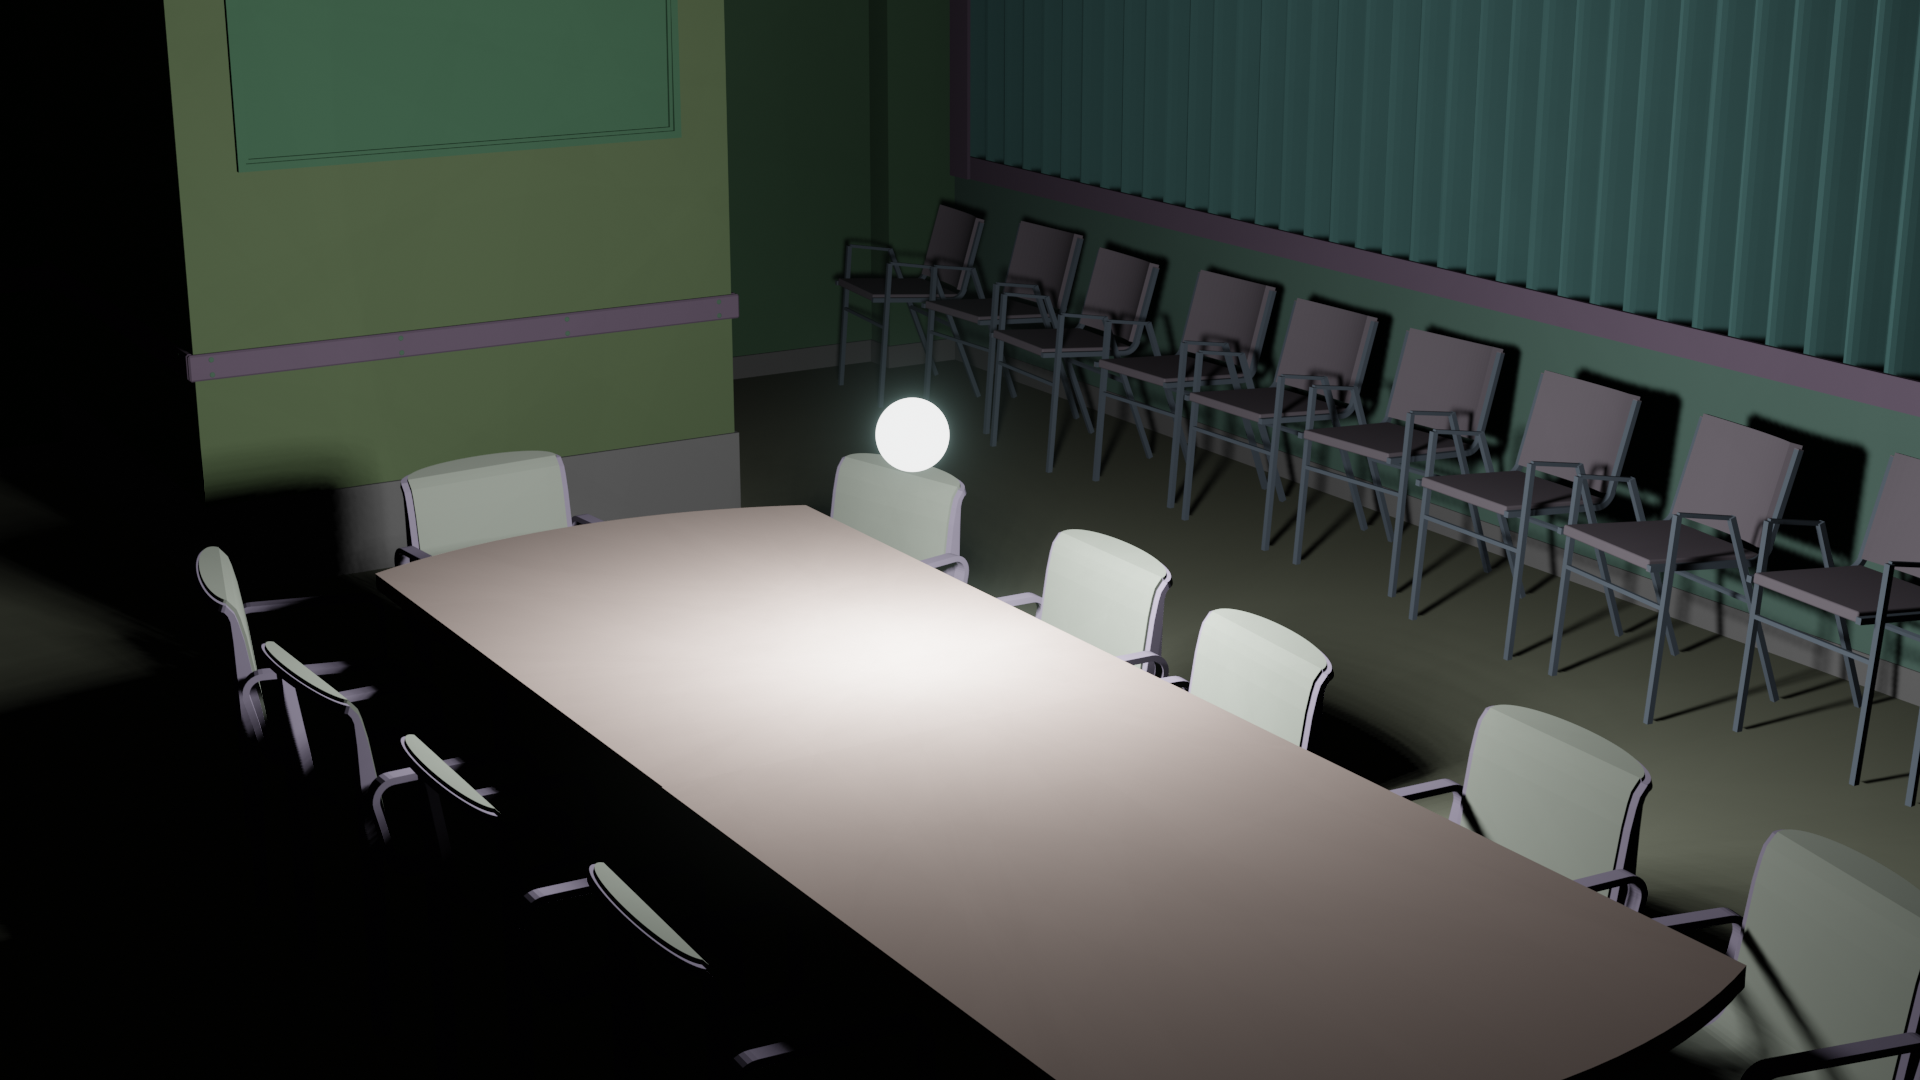
\includegraphics[width=0.475\textwidth]{figures/1 vp.png} \label{fig:1 vp}} \hfill
    \subfigure[2 viewpoints]{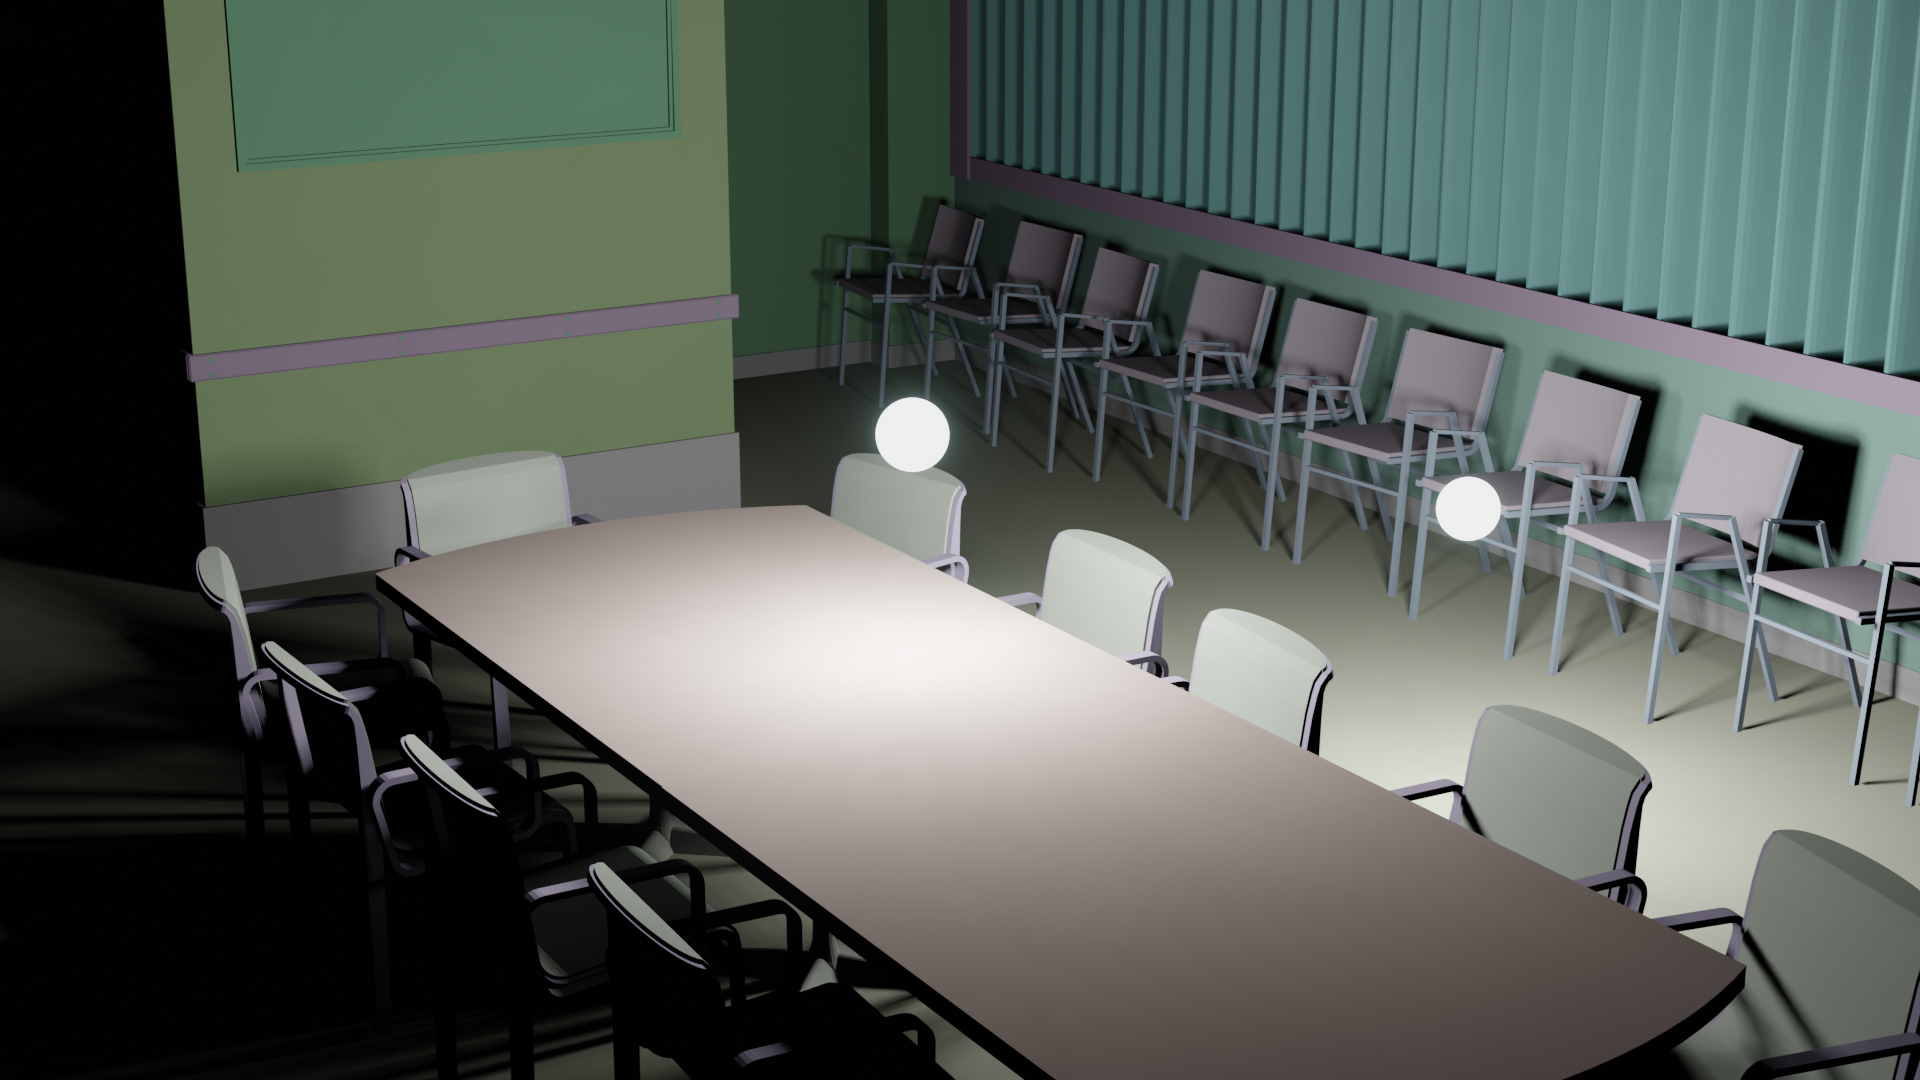
\includegraphics[width=0.475\textwidth]{figures/2 vp.png} \label{fig:2 vp}}
    \caption{Scene with Light Sources}
    \label{fig:scene with light sources}
\end{figure}

\section{Mesh Estimation from Point Cloud} \label{mesh estimation of point cloud}

If we want to apply \textit{occluded area ratio} to point cloud, we have to generate mesh from it. This mesh is certainly only an estimation. Algorithm such as region growing can segment points into clusters based on their properties. With these clusters we can estimate a plane for each of them, then we have a mesh composed by a set of planar primitives. The accuracy of estimation in this step will also affect subsequent process, hence, it's crucial for us to improve the result of mesh estimation. 

\vspace{10pt}

In case of region growing, we need to tweak its input parameters. An example of a code snippet is shown in list \ref{lst:region_growing}, with so many parameters to adjust, the result of region growing can be unstable, which also makes subsequent process difficult to control. Therefore, it's essential to find a more accurate way to estimate mesh.   
\begin{lstlisting}[language=C++, caption=region growing, label=lst:region_growing]
    pcl::RegionGrowing<pcl::PointXYZ, pcl::Normal> reg;
    reg.setMinClusterSize(min_cluster_size);
    reg.setMaxClusterSize(max_cluster_size);
    reg.setSearchMethod(tree);
    reg.setNumberOfNeighbours(num_neighbours);
    reg.setInputCloud(cloud);
    reg.setInputNormals(normals);
    reg.setSmoothnessThreshold(smoothness_threshold / 180.0 * M_PI);
    reg.setCurvatureThreshold(curvature_threshold);
    reg.extract(rg_clusters);
\end{lstlisting}

\section{Generate Point Cloud from Estimated Mesh} \label{generate point cloud from estimated mesh}

Once we have a mesh, we can directly generate points from each face of it. One way to do that is sampling points on polygon, which is normally triangle. We have to make the distribution of points as uniform as possible so that the structural information of mesh can be kept precisely. Otherwise, the generated point cloud will give us distorted information which may lead to significantly biased result of computation. The other way to have points from mesh could be related to ray in the scene. As we mentioned in section \ref{sec:occluded area ratio of mesh}, ray-tracing based mesh can be applied to our pipeline. When there's ray in the scene, we can compute intersections between ray and triangle. These intersections can present structural information of mesh as well, in case of first hit intersection point, we know that the region surrounding this point is visible. This information of visibility may contribute to subsequent computations. 


\section{Boundary Ray Ratio of Point Cloud}

A common way to generate point cloud is conducted by casting lasers from scanner. Since lasers cannot pass through objects, occlusion is then generated on those obscured surfaces. And they are mostly shown on the exterior structure of an indoor scene such as walls, floors and ceilings etc, as they are located in the outermost layer of the room. Items such as chairs and tables, they can also be obscured by other things, but it's difficult to estimate how much they are occluded since their structure is more complex compared to large structures like walls. An example of exterior and interior structure of point cloud is shown in figure \ref{fig:Exterior and interior structure of a point cloud}

\begin{figure}[H]
    \centering
    \subfigure[Exterior]{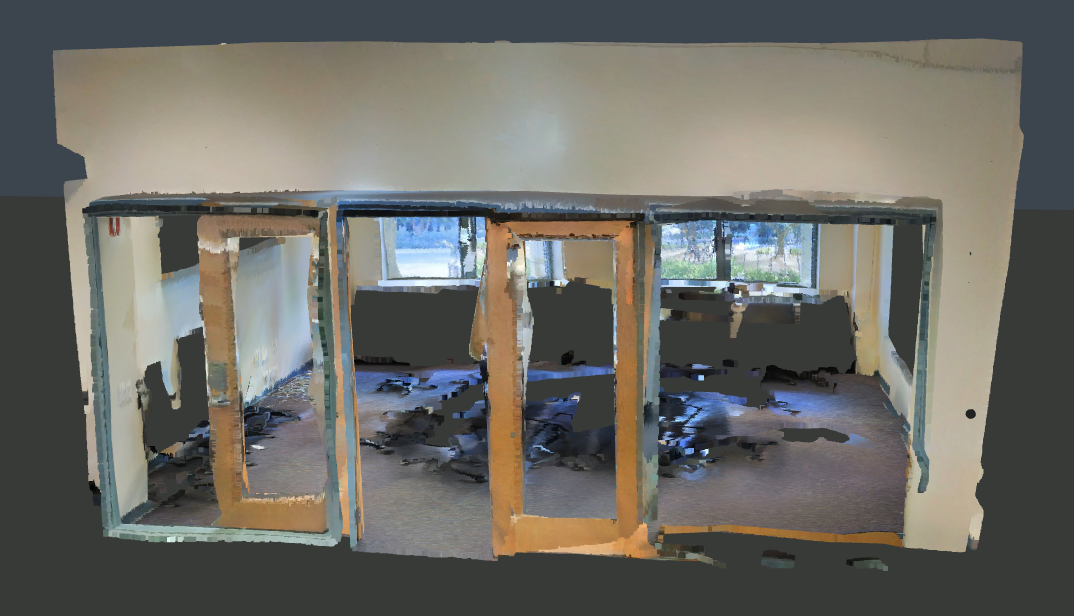
\includegraphics[width=0.65\textwidth]{figures/conf2 ext.png}} \label{fig:exterior} 
    \subfigure[Interior]{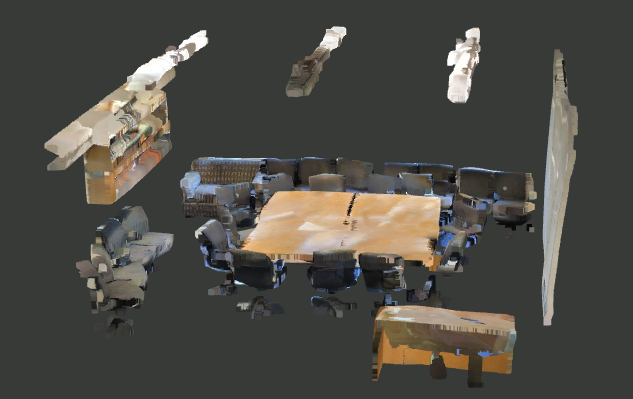
\includegraphics[width=0.65\textwidth]{figures/conf2 int.png}} \label{fig:interior}
    \caption{Scene with Light Sources}
    \label{fig:Exterior and interior structure of a point cloud}
\end{figure}

\vspace{10pt}

Based on what we stated above, we choose \textit{Boundary ray ratio} as the metric to estimate occlusion in point cloud. A set of rays will be cast to detect if it intersect with points identified as exterior structure, in this work we define these external points as boundary. With ground truth labeling of points, the classification of points can easily be done. Finally, we can compute a ratio related to ray that intersects boundary to represent occlusion level of a point cloud. 

\section{Performance Evaluation of Semantic Segmentation} \label{sec:performance evaluation}

This step is to find correlation between occlusion level and performance of semantic segmentation. From previous steps we can already compute occlusion level of a point cloud. The problem here is to use some metrics to evaluate the performance of segmentation. In Section \ref{par:scene flow}, the author of the related work about scene flow, applied F1 score to evaluate their results. This will be considered as one of the options for evaluation. With metrics we computed before we can finally investigate how would the evaluation metrics change with different occlusion level. 

%=====================================================================
\chapter{Technical Solution} \label{chp:solution}
%=====================================================================

In this chapter we will introduce our technical solution to the problem stated in \ref{chp:problem} in a detailed way. The overall workflow is shown below in Figure \ref{fig:overall flowchart of technical solution}.

\begin{figure}[H]
    \centering
    \includegraphics*[width=0.38\textwidth]{figures/technical solution flowchart.png}
    \caption{Overall Flowchart of Technical Solution}
    \label{fig:overall flowchart of technical solution}
\end{figure}

\section{Compute occluded Area Ratio} \label{sec:compute occluded area ratio}

It's difficult to accurately compute occluded area of a triangle, since we don't exactly know which part is visible or invisible geometrically. The method applied here is to sample triangle, with samplings we can have a good coverage of area. Next step is to compute each sampling's visibility to viewpoints in the scene. Then we are able to compute the ratio by counting how many points are invisible. A flow chart of the whole pipeline is shown below in Figure \ref{fig:flowchart of computing occluded area ratio}.

\begin{figure}[H]
    \centering
    \includegraphics*[width=1.0\textwidth]{figures/Compute occluded Area Ratio.png}
    \caption{Flowchart of Computing occluded Area Ratio}
    \label{fig:flowchart of computing occluded area ratio}
\end{figure}

\subsection{Sample Triangles} \label{subsec:sample triangle}

In order to make samplings cover the area of triangle uniformly, we take 2 sampling algorithms into consideration. There are uniform sampling and halton sampling. The only difference of these methods is the way they generate random numbers. With these number we calculate barycentric coordinates based on vertices of triangle. 

\paragraph{Uniform Sampling}

The process begins by randomly generating two parameters, \( r_1 \) and \( r_2 \), both of which lie in the interval [0, 1] with a uniform distribution, ensuring that each point within the interval has an equal probability of being selected. These random parameters are then used to compute the barycentric coordinates of the sampled points within the triangle. The barycentric coordinates, denoted as \( \alpha \), \( \beta \), and \( \gamma \), allow us to express any point within the triangle as a linear combination of the triangle's vertices.

\vspace{10pt}

The algorithm of this part is shown below: 

\begin{algorithm}
\caption{Uniform Sampling within a Triangle}\label{alg:uniform_sampling}
\begin{algorithmic}
\Require Triangle vertices \(V_1\), \(V_2\), \(V_3\)
\Ensure Sampled point \(P\) within the triangle
\State Generate two random numbers \(r_1\) and \(r_2\) with a uniform distribution in the interval [0, 1]
\State Compute the barycentric coordinates using \(r_1\) and \(r_2\) as follows:
\State \hspace{0.5cm} \( \alpha \gets 1 - \sqrt{r_1} \)
\State \hspace{0.5cm} \( \beta \gets \sqrt{r_1} \times r_2 \)
\State \hspace{0.5cm} \( \gamma \gets 1 - \alpha - \beta \)
\State Compute the Cartesian coordinates of the sampled point \(P\) as:
\State \hspace{0.5cm} \( P \gets \alpha V_1 + \beta V_2 + \gamma V_3 \)
\State \Return \(P\)
\end{algorithmic}
\end{algorithm}


\paragraph{Halton Sampling}

In the part of uniform sampling, we have introduced how to compute barycentric coordinates on a triangle. Therefore, here we focus on the generation of random numbers using the Halton sequence, a method that generates quasi-random numbers which are known to fill the space more uniformly compared to purely random numbers.

\vspace{10pt}

The algorithm to generate a number in the Halton sequence can be represented as:

\begin{algorithm}[H]
\caption{Halton Sequence Generation}\label{alg:halton}
\begin{algorithmic}
\Require $index \geq 0$, $base > 1$ (a prime number)
\Ensure Halton number corresponding to the given index and base
\State $result \gets 0.0$
\State $f \gets 1.0 / base$
\State $i \gets index$
\While{$i > 0$}
    \State $result \gets result + f \cdot (i \mod base)$
    \State $i \gets i / base$  \Comment{Integer division}
    \State $f \gets f / base$
\EndWhile
\State \Return $result$
\end{algorithmic}
\end{algorithm}


Using this method, we generate two sequences of Halton numbers with different bases such as 2 and 3, respectively, which are then used to compute the barycentric coordinates for uniform sampling within a triangle. These quasi-random numbers, \( r1 \) and \( r2 \), provide a more evenly distributed set of sample points within the triangle compared to purely random sampling, facilitating a more uniform sampling process. This can be verified in Figure \ref{fig:sample triangle}, where halton sampling shows a result which is closer to even distribution.  

\begin{figure}[H]
    \centering
    \subfigure[Uniform]{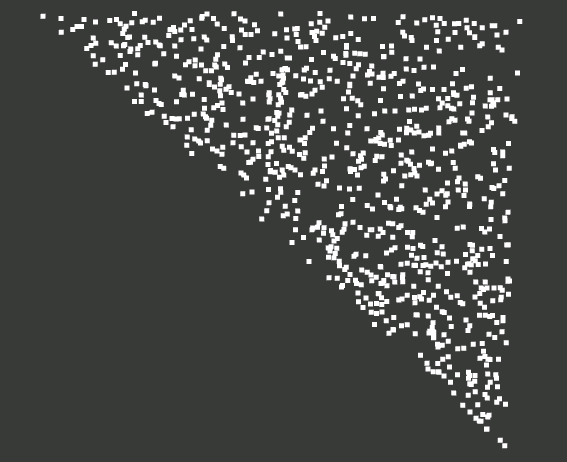
\includegraphics[width=0.7\textwidth]{figures/uniform sample triangle.png}}  \label{fig:uniform sampling} 
    \subfigure[Halton]{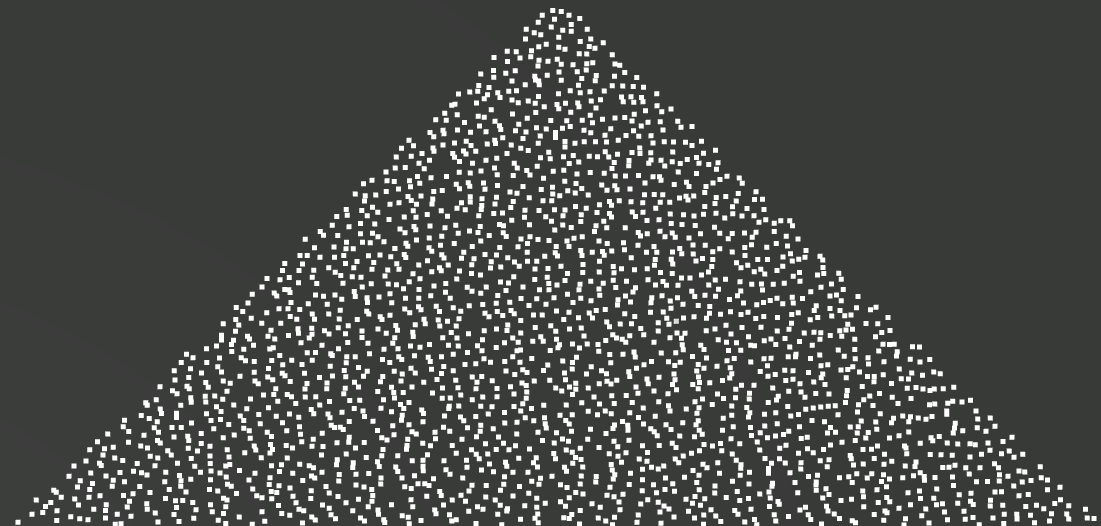
\includegraphics[width=0.7\textwidth]{figures/halton sample triangle.png}} \label{fig:halton sampling}
    \caption{Sample Triangle}
    \label{fig:sample triangle}
\end{figure}



\subsection{Generate Rays}

Rays simulate the path of light as it interacts with objects in a scene. In our approach, while it's an usual case to cast ray from viewpoint, here we generate them from the sampled points on the triangle to the light source as shown in Figure \ref{fig:generate ray from sampling to viewpoint}, we need to pay attention that the viewpoint is abstracted as a point instead of an object with volume. The sampled points serve as the origin of each ray, while the view point (or light source) acts as the look-at point. The direction of each ray is computed based on the difference between the viewpoint and the origin. The direction vector is then normalized to ensure its magnitude is 1, which simplifies subsequent calculations.

\vspace{10pt}

The direction vector can be calculated using the formula 
\[
\textit{Direction} = \frac{\textit{viewpoint} - \textit{Origin}}{\|\textit{viewpoint} - \textit{Origin}\|}
\]

Where:
\begin{itemize}
    \item \(\textit{Origin}\) is the starting point of the ray, which in our case is the sampled point on the triangle.
    \item \(\textit{Destination}\) is the end point of the ray, typically representing the viewpoint or light source.
\end{itemize}

\begin{figure}[H]
    \centering
    \includegraphics*[width=0.5\textwidth]{figures/sample to vp.png}
    \caption{Generate Ray from Sampling to Viewpoint}
    \label{fig:generate ray from sampling to viewpoint}
\end{figure}

When there are multiple viewpoints in the scene, we have to generate same amount of rays as viewpoints for each sampling.  

\subsection{Ray Triangle Intersection}

Ray-triangle intersection is a fundamental operation in computer graphics, especially in the context of ray tracing. Determining whether a ray intersects a triangle and finding the intersection point are crucial for rendering scenes composed of triangular meshes.
\vspace{10pt}

One of the most efficient and widely used algorithms for this purpose is the \textit{Möller–Trumbore} intersection algorithm. It operates by representing the triangle in barycentric coordinates, which allows it to avoid the computation of explicit plane equations. It then uses these coordinates to find the intersection point of the ray and the triangle, if it exists. The algorithm performs a series of vector operations including dot products and cross products to compute the barycentric coordinates and the distance from the ray's origin to the intersection point. More detail is shown below:

\vspace{10pt}

\begin{algorithm}[H]
\caption{Möller–Trumbore Ray-Triangle Intersection Algorithm}\label{alg:ray_triangle_intersection}
\begin{algorithmic}
\Require Ray with origin \( O \) and direction \( D \)
\Require Triangle with vertices \( V_1 \), \( V_2 \), and \( V_3 \)
\Ensure Intersection point \( P \) or indication of no intersection

\State Compute edge vectors:
\State \hspace{0.5cm} \( e_1 \gets V_2 - V_1 \)
\State \hspace{0.5cm} \( e_2 \gets V_3 - V_1 \)

\State Compute vector \( h \) as the cross product of \( D \) and \( e_2 \):
\State \hspace{0.5cm} \( h \gets D \times e_2 \)

\State Compute determinant \( a \):
\State \hspace{0.5cm} \( a \gets e_1 \cdot h \)

\If{\( a \) is close to zero}
    \State \Return No intersection  \Comment{Ray is nearly parallel to the triangle}
\EndIf

\State Compute factor \( f \):
\State \hspace{0.5cm} \( f \gets \frac{1}{a} \)

\State Compute vector \( s \):
\State \hspace{0.5cm} \( s \gets O - V_1 \)

\State Compute barycentric coordinate \( u \):
\State \hspace{0.5cm} \( u \gets f \cdot (s \cdot h) \)

\If{\( u < 0 \) or \( u > 1 \)}
    \State \Return No intersection
\EndIf

\State Compute vector \( q \) as the cross product of \( s \) and \( e_1 \):
\State \hspace{0.5cm} \( q \gets s \times e_1 \)

\State Compute barycentric coordinate \( v \):
\State \hspace{0.5cm} \( v \gets f \cdot (D \cdot q) \)

\If{\( v < 0 \) or \( u + v > 1 \)}
    \State \Return No intersection
\EndIf

\State Compute distance \( t \) to the intersection point:
\State \hspace{0.5cm} \( t \gets f \cdot (e_2 \cdot q) \)

\State Compute intersection point \( P \):
\State \hspace{0.5cm} \( P \gets (1 - u - v) V_1 + u V_2 + v V_3 \)

\State \Return Intersection point \( P \) and distance \( t \)
\end{algorithmic}
\end{algorithm}

\subsection{Occluded Area Ratio}

From previous steps, we have computed samplings on each triangle and generated rays originating from these samplings directed towards the viewpoints. As opposed to directly compute occluded area, we detect visible samplings here. We use visible weight represents the ratio of visible samplings to the total number of samplings on the triangle. With this weight we compute visible area for each triangle, then we sum up them to get the total visible area, and the ratio can be easily calculated with total area. Mathematically, the visibility weight, \( w \), can be defined as:
\[ 
    w = \frac{\textit{Number of visible samplings per triangle}}{\textit{Total number of samplings per triangle}}
\]

The visible area \( A_{\textit{visible}} \) of the triangle can then be computed as:
\[ 
    A_{\textit{visible}} = w \times A_{\textit{total}}
\]

The visible area ratio, denoted as \( R_{\textit{visible}} \), is calculated as the ratio of the total visible area \( A_{\textit{total visible}} \) to the total area \( A_{\textit{total}} \) of the triangle. It can be mathematically represented as:
\[ 
    R_{\textit{visible}} = \frac{A_{\textit{total visible}}}{A_{\textit{total}}}
\]

Conversely, the occluded area ratio, denoted as \( R_{\textit{occluded}} \), can be calculated as the complement of the visible area ratio. It is given by:
\[ 
    R_{\textit{occluded}} = 1 - R_{\textit{visible}}
\]

A sampling is deemed visible if at least one ray originating from it does not intersect any triangle between its origin and the viewpoint other than the one from which the sampling was generated. To ascertain this, we should examine all first hit intersection related to the ray cast from the sampling. If the distance from origin to viewpoint is shorter than the distance between origin and first hit intersection, which means no intersection can obscure the viewpoint, then this sampling is considered visible. 

\begin{algorithm}[H]
\caption{Determining the Visibility of a Sampling}\label{alg:visibility_sampling}
\begin{algorithmic}
\Require Ray originating from sampling with origin \( O \) and direction \( D \)
\Require Viewpoint \( V \)
\Require Set of triangles \( T \) excluding the triangle from which the sampling was generated
\Ensure Visibility status of the sampling

\State Compute the distance from the origin to the viewpoint: \( d_{\text{viewpoint}} = \| V - O \| \)
\State Initialize variable \( d_{\text{intersection}} \) to infinity
\State Initialize variable \( \text{isVisible} \) to false

\For{each triangle \( t \) in \( T \)}
    \State Compute the intersection of the ray with triangle \( t \) using the Möller–Trumbore algorithm
    \If{there is an intersection at distance \( d \) from \( O \)}
        \State Update \( d_{\text{intersection}} \) to the minimum of \( d_{\text{intersection}} \) and \( d \)
    \EndIf
\EndFor

\If{\( d_{\text{viewpoint}} < d_{\text{intersection}} \)}
    \State Set \( \text{isVisible} \) to true  \Comment{No intersection obscures the viewpoint}
\EndIf

\State \Return \( \text{isVisible} \)
\end{algorithmic}
\end{algorithm}
 
\section{Estimate Mesh and Generate Point Cloud} \label{sec:estimate mesh and generate point cloud}

In this part we estimate mesh for subsequent computation of occluded area ratio. Since we want to make comparison between this ratio and occlusion level of point cloud, the cloud should be generated from this mesh. 

\subsection{Estimate Mesh from Point Cloud} \label{par:estimate mesh from point cloud}

As discussed in \ref{mesh estimation of point cloud}, region growing is an option here to segment points and to fit planar primitives based on segmented clusters of points, but the result is difficult to control, and the process of fitting plane from clusters might increase its instability. An alternative could be the work has been done by Mulin and Florent[GoCoPP], they proposed a method \textit{GoCoPP} to find good configurations of planar primitives in unorganized point cloud. Regarding their experiments, \textit{GoCoPP} outperforms region growing on different evaluation metrics. Below in Figure \ref{segmentation results} shows the result of 2 methods where in case of region growing we only segmented the point cloud, while in \textit{GoCoPP} they already triangulated planar primitive by applying alpha shape algorithm. With the triangulated mesh we can directly feed this data into our pipeline. Therefore, we choose to apply \textit{GoCoPP} to generate mesh from point cloud.

\begin{figure}[H]
    \centering
    \subfigure[Region Growing]{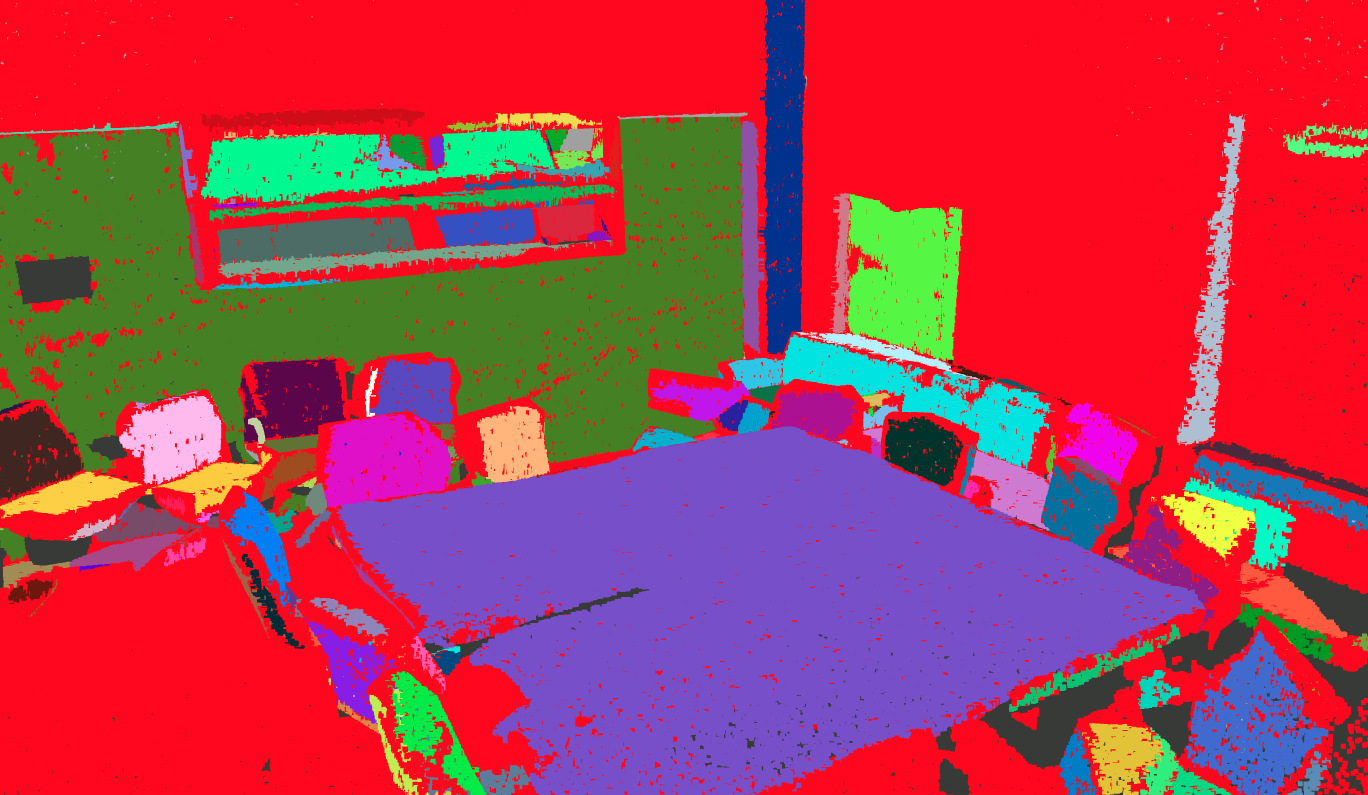
\includegraphics[width=0.65\textwidth]{figures/conf2 rg.png}}  \label{fig:region growing} 
    \subfigure[GoCoPP]{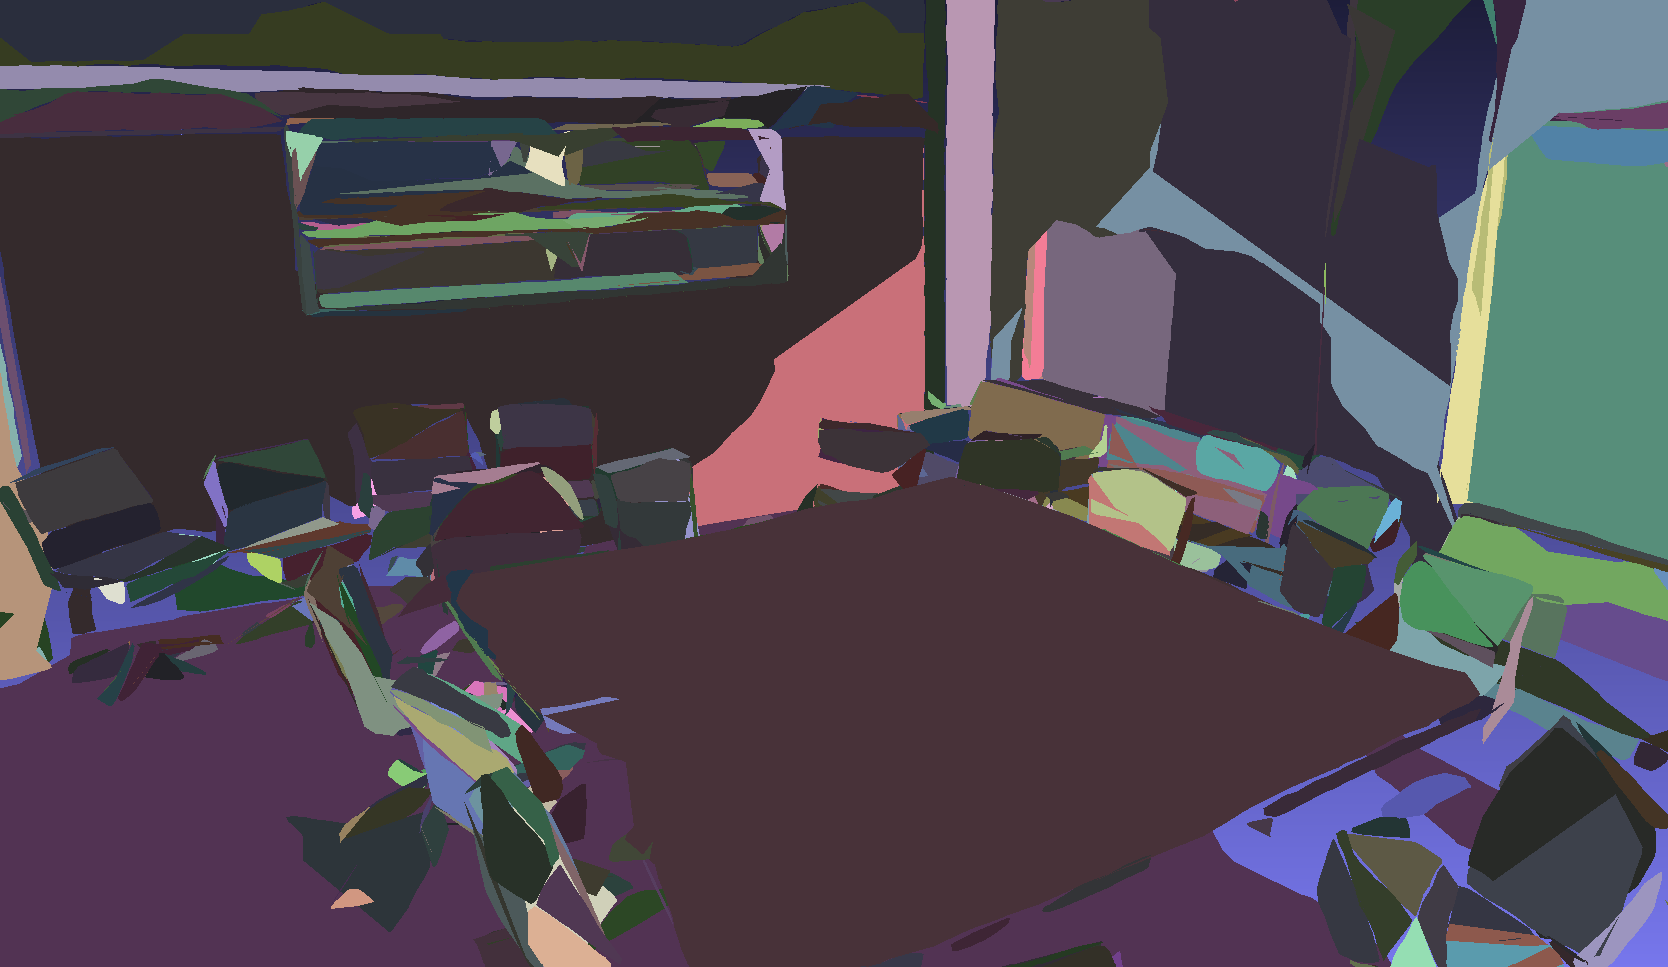
\includegraphics[width=0.65\textwidth]{figures/conf2 gocopp.png}} \label{fig:gocopp}
    \caption{Segmentation Methods}
    \label{segmentation results}
\end{figure}

We use the same pipeline introduced in \ref{sec:compute occluded area ratio} to compute its occluded area ratio to represent occlusion level. The result depends on which strategy we use to place viewpoints. We can randomly place them in the scene or with fixed position such as center of the scene's bounding box, this will be explained more detailed in \ref{chp:experimental results}.

\subsection{Generate Point Cloud from Estimated Mesh} \label{par:generate point cloud from estimated mesh}

The computation of occluded area of a mesh is based on visible samples on each triangle. Since we want to make comparison on occlusion level between mesh and point cloud, the cloud should reflect the information about visibility. Hence, here we directly create the visible point cloud from visible samplings.

\section{Compute Boundary Ray Ratio of Point Cloud} \label{compute boundary ray ratio of point cloud} 

We define the boundary ray as the ray which intersects with boundary point. Although our input point cloud has ground truth label of each point, the cloud created from samplings does not preserve this kind of information. Therefore, the first step is to identify the semantic class of each point. With these information we can then compute if a ray intersects with boundary. A workflow of this part is shown in Figure \ref{fig:flowchart of computing boundary ray ratio}.

\begin{figure}[H]
    \centering
    \includegraphics*[width=0.85\textwidth]{figures/Compute Boundary Ray Ratio of Point Cloud.png}
    \caption{Flowchart of Computing Boundary Ray Ratio}
    \label{fig:flowchart of computing boundary ray ratio}
\end{figure}

\subsection{Estimate Semantics}

We have to first categorize point of the original ground truth cloud into either boundary or non-boundary. 
Then we put the point of visible sampling cloud inside the pre-processed boundary cloud. To determine the category we compute nearest neighbours of a point, if there are more boundary points we classify it as boundary as well, and vice versa. The computation of nearest neighbours is realized through \textit{K-D Tree} algorithm, which offers us an efficient way to get a search point's \textit{K} nearest neighbour points, where \textit{K} indicate the number of neighbours.


\subsection{Generate Random Rays}

We want to use a ray from outside of the scene and directed towards the cloud, then we check how many boundaries the ray can intersects with, since this indicate how much occlusion a ray can contribute to the overall occlusion level. In case of a room, its boundary can be represented as a cuboid, which can at most has 2 faces intersect with one ray. Based on that, our rays can be classified as \textit{non-boundary ray}, \textit{1-boundary ray} and \textit{2-boundary ray} as shown in Figure \ref{classification of bound ray}

\begin{figure}[H]
    \centering
    \subfigure[Non-boundary Ray]{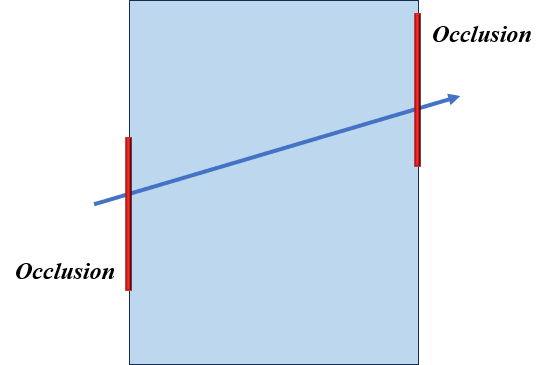
\includegraphics[width=0.32\textwidth]{figures/no bound.png}} \label{fig:non-bound ray}
    \subfigure[1-boundary Ray]{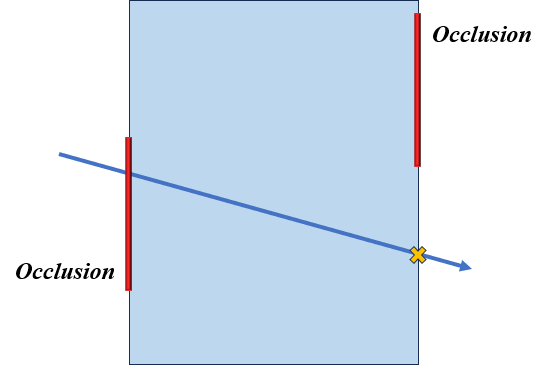
\includegraphics[width=0.32\textwidth]{figures/1 bound.png}} \label{fig:1-bound ray}
    \subfigure[2-boundary Ray]{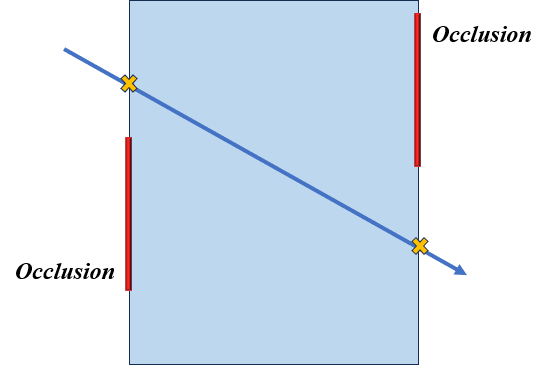
\includegraphics[width=0.32\textwidth]{figures/2 bounds.png}}  \label{fig:2-bounds ray} 
    \caption{Classification of Boundary Rays}
    \label{classification of bound ray}
\end{figure}

\vspace{10pt}

In our work, it's more feasible for us to create rays within the room which is always presented as point cloud. We first randomly generate two points within the bounding box of the scene. One as origin of the ray and the other is the look-at direction. To simulate a ray originates from outside and pass through the room we also take its opposite direction into consideration. Namely, for one ray we have to compute its intersection with points in both directions. 

\begin{figure}[H]
    \centering
    \includegraphics*[width=0.5\textwidth]{figures/ray with two directions.png}
    \caption{Ray with 2 Directions}
    \label{fig:ray with 2 directions}
\end{figure}

\subsection{Ray Point Intersection} \label{ray point intersection}

Each point within the point cloud is represented as a small sphere with a defined radius. This simplifies the ray-point intersection check, as we can treat each point as a volumetric entity rather than a singular coordinate in space. The way ray intersects with a sphere is illustrated in Figure \ref{fig:ray intersect point}. 

\begin{figure}[H]
    \centering
    \includegraphics*[width=0.32\textwidth]{figures/ray intersect point.png}
    \caption{Ray Intersect Point}
    \label{fig:ray intersect point}
\end{figure}

To determine if a ray intersects with a sphere, we follow algorithm stated below:

\begin{algorithm}[H]
\caption{Ray-Sphere Intersection Algorithm}
\begin{algorithmic}[1]
\Require Ray origin, Ray direction, Sphere center, Sphere radius
\State Normalize the ray direction vector if not normalized
\State Compute vector \( \mathbf{L} = \text{Sphere center} - \text{Ray origin} \)
\State Compute \( \text{originDistance}^2 = \mathbf{L} \cdot \mathbf{L} \)
\State Compute \( t_{ca} = \mathbf{L} \cdot \text{Normalized ray direction} \)
\If{\( \text{originDistance}^2 < \text{Sphere radius}^2 \)}
    \State \Return Intersection exists (Ray origin is inside the sphere)
\EndIf
\If{\( t_{ca} < 0 \)}
    \State \Return No intersection (Sphere is behind the ray)
\EndIf
\State Compute \( d^2 = \text{originDistance}^2 - t_{ca}^2 \)
\If{\( d^2 > \text{Sphere radius}^2 \)}
    \State \Return No intersection (Ray misses the sphere)
\Else
    \State \Return Intersection exists (Ray intersects the sphere)
\EndIf
\end{algorithmic}
\end{algorithm}


\subsection{Ray Openings Intersection}

Openings or gaps in the scene, such as windows or doors, should not contribute to occlusion. In the context of boundary rays, we regard openings as boundary. To account for these openings, we need an efficient method to determine if a ray intersects with any of the openings in the scene. Given the typically limited number of openings in a scene, it's feasible to manually select a few points that represent the boundary of each opening. Using these points, we can construct a polygonal representation of the opening. The ray-openings intersection check can then be performed by testing if the ray intersects with any of these polygons.

\vspace{10pt}

For a set of points \( P = \{p_1, p_2, ..., p_n\} \) that define a polygon, we first estimate a plane \( \mathbf{N} \) that best fits these points. Once the plane is determined, all points are projected onto this plane to ensure they lie within the same plane. The next step involves calculating the intersection of the ray with this plane. If an intersection exists, we need to determine if this intersection point lies inside the polygon. This workflow is shown in Figure \ref{fig:estimate polygon from points}.

\begin{figure}[H]
    \centering
    \includegraphics*[width=1.0\textwidth]{figures/detect openings.png}
    \caption{Estimate Polygon from Points}
    \label{fig:estimate polygon from points}
\end{figure}

To check the position of the intersection point relative to the polygon, we construct vectors between the intersection point and each vertex of the polygon. For every pair of neighboring vectors, we compute their cross product. If all resulting cross products point in the same direction (i.e., they have the same sign), then the intersection point is inside the polygon. Otherwise, the intersection point lies outside the polygon.

\vspace{10pt}

Mathematically, given two vectors \( \mathbf{v_1} \) and \( \mathbf{v_2} \), their cross product is given by:
\[
\mathbf{v_1} \times \mathbf{v_2} = \begin{vmatrix}
\mathbf{i} & \mathbf{j} & \mathbf{k} \\
v_{1x} & v_{1y} & v_{1z} \\
v_{2x} & v_{2y} & v_{2z} \\
\end{vmatrix}
\]
Where \( \mathbf{i}, \mathbf{j}, \) and \( \mathbf{k} \) are the unit vectors in the x, y, and z directions, respectively. By iterating over all the vertices of the polygon and computing these cross products, we can determine the position of the intersection point with respect to the polygon. In Figure \ref{fig:ray intersect polygon} the ray intersects with polygon. To verify the algorithm with this illustration, we can apply right-hand rule to every 2 neighbouring vectors in clockwise order, then the cross product should always point downwards.

\begin{figure}[H]
    \centering
    \includegraphics*[width=0.25\textwidth]{figures/intersect polygon.png}
    \caption{Ray Intersect Polygon}
    \label{fig:ray intersect polygon}
\end{figure}

\subsection{Boundary Ray Ratio}

The ray within a scene may intersect with multiple boundary points or openings. In our approach, since we have defined the classification of rays with at most 2 boundaries, we only inspect whether each ray intersects with a boundary in each direction. Specifically, if a ray intersects boundaries in both directions, it is classified as a 2-boundary ray.

\vspace{10pt}

After classifying all rays in the scene, we compute the boundary ray ratio, which exactly represents the occlusion level of a point cloud, using the following formula:

\[
\textit{{Boundary Ray Ratio}} = \frac{{\textit{{occlusion}}}}{{\textit{{occlusion}} + \textit{{visibility}}}} = \textit{{Occlusion Level}}
\]

Where:
\begin{itemize}
    \item \textbf{{Occlusion}}: The number of rays that do not intersect with any boundary, denoted as \textit{{non-boundary ray count}}.
    \item \textbf{{Visibility}}: A measure calculated as the sum of \textit{{1-boundary ray count}} and twice the \textit{{2-boundary ray count}}.
\end{itemize}

The quantities in the formula are calculated as follows:
\[
    \textit{{occlusion}} = \textit{{non-boundary ray count}}
\]
\[
    \textit{{visibility}} = \textit{{1-boundary ray count}} + 2 \cdot \textit{{2-boundary ray count}} \FIXME{change the formula}
\]

By evaluating the occlusion level with the above formula, we can analyze the proportion of rays that are obstructed versus those that are not, providing insight into the level of visibility within the scene.


\section{Evaluate Performance of Segmentation} \label{evaluate performance of segmentation}

In this step, we are going to compare performance of segmentation of point clouds with different occlusion level. Since the complexity and structure of each room scene can vary greatly, we want to do the comparisons within the same scene but with different occlusion level. To achieve this we would create a set of sub-sampled point clouds based on number of viewpoints in the scene.

\subsection{Ray Tracing Based Point Cloud Scanning} \label{sec:ray tracing point cloud scanning}

To down-sample the original point cloud, we would perform it in a manner similar to sampling a real scene using a laser scanner. The points stored in the data acquired from the scanner are those that are visible to it. If we apply this to original point cloud, we are actually creating a sub-sampled data set based on visibility to light sources. 

\paragraph{Spherical Light Source}

To simulate a light source that emits rays in all directions, we use a spherical model. Points are sampled on the surface of this sphere using the Halton sequence, which we introduced in Algorithm \ref{alg:halton}. Each point represents a direction for a ray. The number of rays (or sampled points) is predetermined and can be adjusted based on the desired resolution or accuracy of the scan. An example of the result of this method is shown in Figure \ref{fig:halton sample sphere}.

\begin{figure}[H]
    \centering
    \includegraphics*[width=0.4\textwidth]{figures/halton sample sphere.png}
    \caption{Halton Sample Sphere}
    \label{fig:halton sample sphere}
\end{figure}

The sampling on the sphere is achieved using halton sampling in the azimuthal (\( \theta \)) and polar (\( \phi \)) angles. This method ensures a uniform distribution of points over the sphere's surface, providing a comprehensive representation of the light source's emission pattern. The coordinates of a sampled point on the sphere are computed based on the center point of the sphere and a predefined radius. The specific algorithm is as follows:

\begin{algorithm}[H]
\caption{Halton Sampling on Sphere Surface}
\begin{algorithmic}[1]
\Require Sphere center, Number of samples, Radius
\State Initialize an empty list of samples
\For{\(i = 0\) to \( \text{number of samples} - 1\)}
    \State Compute azimuthal angle \( \theta = 2 \pi \times \text{halton}(i, 2) \)
    \State Compute polar angle \( \phi = \arccos(2 \times \text{halton}(i, 3) - 1) \)
    \State Compute sample point coordinates:
    \State \( x = \text{center.x} + \text{radius} \times \sin(\phi) \times \cos(\theta) \)
    \State \( y = \text{center.y} + \text{radius} \times \sin(\phi) \times \sin(\theta) \)
    \State \( z = \text{center.z} + \text{radius} \times \cos(\phi) \)
    \State Add the computed point to the samples list
\EndFor
\State Set the properties of the point cloud (width, height, and density)
\State \Return the list of samples
\end{algorithmic}
\end{algorithm}

\subsection{Evaluate Performance with Metrics}

Evaluating the performance of semantic segmentation is crucial to ensure its reliability and effectiveness. Metrics serve as standardized measures to assess the quality of segmentation results, comparing the predicted outputs against the ground truth. In this part, we discuss the metrics used to evaluate the performance of semantic segmentation models.

\paragraph{Semantic Classes}

Semantic segmentation requires a clear definition of the classes that are to be identified within the data set. Due to discrepancies between the ground truth point cloud data set, denoted as [S3dis], and the data set used for the pre-trained model, we have extracted those common semantic classes for our segmentation task in Table \ref{tab:semantic_classes}:

\begin{table}[H]
    \centering
    \begin{tabular}{|c|c|}
        \hline
        \textbf{Semantic Class} & \textbf{Class ID} \\
        \hline
        Wall & 0 \\
        Floor & 1 \\
        Ceiling & 1 \\
        Chair & 4 \\
        Sofa & 5 \\
        Table & 6 \\
        Door & 7 \\
        Window & 8 \\
        Bookcase & 9 \\
        Beam & 20 \\
        Board & 21 \\
        Clutter & 25 \\
        Column & 26 \\
        \hline
    \end{tabular}
    \caption{Mapping of semantic classes to their respective class IDs.}
    \label{tab:semantic_classes}
\end{table}

Given a segmented point cloud, we can evaluate the segmentation by calculating various metrics such as accuracy, precision, and recall for each class. In semantic segmentation of point clouds, each point in the cloud is classified into one of several possible categories, which are True Positives (TP), False Positives (FP), True Negatives (TN), and False Negatives (FN) regarding the correctness of segmentation. The Algorithm \ref{alg:computation of tp, tn, fp, fn} demonstrates how to classify points into them and counting the values. With these values we can then compute metrics explained in subsequent section.  

\begin{algorithm}[H]
\caption{Computation of TP, TN, FP, and FN for Point} \label{alg:computation of tp, tn, fp, fn}
\begin{algorithmic}[1]
\Require Segmented point cloud \(P\) with \(N\) points, Ground truth labels for each point
\Ensure Computation of True Positives (TP), True Negatives (TN), False Positives (FP), and False Negatives (FN) for each class

\State Initialize counters for True Positives (TP), True Negatives (TN), False Positives (FP), and False Negatives (FN) for each class to zero
\For{each point \(p_i\) in point cloud \(P\)}
    \State Get the ground truth label and predicted label for \(p_i\)
    \For{each class \(c_j\)}
        \If{the ground truth label of \(p_i\) is \(c_j\)}
            \If{the predicted label of \(p_i\) is \(c_j\)}
                \State TP for class \(c_j\) += 1
            \Else
                \State FN for class \(c_j\) += 1
            \EndIf
        \Else
            \If{the predicted label of \(p_i\) is \(c_j\)}
                \State FP for class \(c_j\) += 1
            \Else
                \State TN for class \(c_j\) += 1
            \EndIf
        \EndIf
    \EndFor
\EndFor

\State \Return Counters TP, TN, FP, and FN for each class
\end{algorithmic}
\end{algorithm}

\paragraph{Metrics} \label{par:metrics}

To evaluate the performance of our model in the context of point cloud segmentation, we employ several widely-recognized metrics, which includes \textit{Accuracy}, \textit{IoU}, \textit{Precision}, \textit{Recall} and \textit{F1 Score}. 

\vspace{10pt}

These metrics provide different perspectives on the model's capabilities and are computed using the values of True Positives (TP), False Positives (FP), True Negatives (TN), and False Negatives (FN) which are obtained for each class through the algorithm described earlier. Below, we detail these metrics along with their respective mathematical formulations:

\vspace{10pt}

\textbf{Accuracy} is a fundamental metric that quantifies the proportion of correctly predicted points out of the total number of points. It is given by the formula:
\[
    \textit{Accuracy} = \frac{\textit{Number of Correct Predictions}}{\textit{Total Number of Predictions}}
\]
which can also be formulated in terms of TP, FP, TN and FN as:
\[
    \textit{Accuracy} = \frac{TP + TN}{TP + TN + FP + FN}
\]

Though a useful metric, accuracy can sometimes be misleading, particularly when the classes are imbalanced.

\vspace{10pt}

\textbf{IoU (Intersection over Union)}, also known as the Jaccard Index, measures the overlap between the predicted segmentation and the ground truth. It is calculated as the area of overlap divided by the area of union of the two sets, as given by:
\[
    IoU = \frac{\textit{Intersection}}{\textit{Union}}
\]
or equivalently,
\[
    IoU = \frac{TP}{TP + FP + FN}
\]

A higher IoU value signifies better segmentation accuracy.

\vspace{10pt}

\textbf{Precision and Recall} are two complementary metrics that provide insights into the model's performance regarding false positives and false negatives. 

\vspace{10pt}

\textbf{Precision} quantifies the proportion of positive identifications that were actually correct, as given by:
\[
    \textit{Precision} = \frac{\textit{True Positives}}{\textit{True Positives} + \textit{False Positives}}
\]
or equivalently,
\[
    \textit{Precision} = \frac{TP}{TP + FP}
\]

A higher precision indicates a larger percentage of the model's positive predictions were correct.

\vspace{10pt}

\textbf{Recall}, on the other hand, measures the proportion of actual positives that were identified correctly, as given by:
\[
    \textit{Recall} = \frac{\textit{True Positives}}{\textit{True Positives} + \textit{False Negatives}}
\]
or equivalently,
\[
    \textit{Recall} = \frac{TP}{TP + FN}
\]

A higher recall indicates that fewer actual positives were missed by the model.

\vspace{10pt}

\textbf{F1 Score} is the harmonic mean of precision and recall, providing a balance between the two and ensuring that both false positives and false negatives are considered. It is calculated as:
\[
    F1 = 2 \times \frac{\textit{Precision} \times \textit{Recall}}{\textit{Precision} + \textit{Recall}}
\]
or equivalently,
\[
    F1 = 2 \times \frac{TP}{2 \times TP + FP + FN}
\]

An F1 Score closer to 1 indicates better performance, while a score closer to 0 indicates poor performance.

%=====================================================================
\chapter{Implementation}\label{chp:implementation}
%=====================================================================

In this chapter, we first delve deeper into the core part of implementation of our computational pipeline as presented in Chapter \ref{chp:solution}. Then we go through the overall structure of the software which is ready for user to interact with.

\section{PCL and Eigen Serves for Computation}\label{sec:pcl and eigen}

The Point Cloud Library (PCL) stands as the backbone of our implementation. We rely on PCL to accomplish a set of tasks, ranging from reading point cloud to evaluating its occlusion levels. Parallel to PCL, the Eigen library emerges as an invaluable asset. It is our preferred choice for handling mathematical operations that are indispensable to our pipeline.

\subsection{Handling Point Cloud Data}

We read point cloud data and load them into different types as follows:

\begin{itemize}
    \item \textbf{pcl::PointXYZ} - Point cloud with only coordinate information.
    \item \textbf{pcl::PointXYZI} - Extra intensity field, in this work it is used mostly to store category information of a point.
    \item \textbf{pcl::PointXYZRGB} - Point cloud with coordinate and color information. If without RGB value attached, we will see point cloud rendered with white color.
\end{itemize}

Sometimes we need to store points to a new point cloud, which can be done in a typical way shown in code snippet below:

\begin{lstlisting}[language=C++, caption=Save Point Cloud Data]
pcl::PointCloud<pcl::PointXYZ>::Ptr cloud(new pcl::PointCloud<pcl::PointXYZ>);
for(...) {
    pcl::PointXYZ point;
    cloud->points.push_back(point);
}
cloud->width = cloud->points.size();
cloud->height = 1;
cloud->is_dense = true;
pcl::io::savePCDFileASCII("../files/cloud.pcd", *cloud);
\end{lstlisting}

\subsection{Estimate Polygon}

Computation of ray-opening intersection plays an crucial role in calculating boundary ray ratio. Each opening is represented as a polygon, and the data we can extract from the original point cloud is a set of small clouds where each point inside it can be regarded as a vertex of polygon in 3D space. And these vertices are most likely not in the same plane, therefore, we would estimate a polygon which is able to be used in subsequent computation. 

\paragraph{Plane Estimation}

The initial step is fitting a plane to each cluster's point data. For this, we rely on the RANSAC algorithm embedded within PCL. In the code snippet shown below, PCL's \textit{SACSegmentation} is configured to detect planar models. If successful, it retrieves the plane's coefficients.

\paragraph{Formation of Polygon}

With the plane's coefficients, our next move is to project every point in the cluster onto this plane. This ensures that all points lie in a co-planar fashion. Once our points sharing a planar space, we compute the convex hull of each cluster. This results in a 2D polygon within a 3D space, effectively enveloping all the cluster points.

Here, PCL's \textit{ProjectInliers} projects the points onto the detected plane, thereby creating a co-planar point cloud, which we refer to as \textit{cloud projected}. The usage of PCL's \textit{ConvexHull} class create a cloud representing the polygon.


\subsection{Ray Tracing Based Intersection Computation} \label{sec:ray tracing}

Ray tracing based methods are pivotal to our computational pipeline. We use ray to check if it intersects with any basic element in the scene, such as point, triangle, polygon, bounding box, etc.

\paragraph{Database-like Structure}

To compute and record all intersections between all rays and all elements in the scene, we build different structure for each type of element. Their interactions are also stored, which makes the system appears to be a relational database. We can query this database to get all the information we need.  

\begin{lstlisting} [language=C++, caption=Data Structures, label=lst:database]
struct Ray3D {      // ray structure used for point cloud ray tracing
    size_t index;
    pcl::PointXYZ origin;
    pcl::PointXYZ direction;
    std::vector<size_t> first_dir_bound_intersection_idx;
    std::vector<size_t> second_dir_bound_intersection_idx;
    ...
};
struct Intersection {
    size_t index;
    size_t triangle_index;
    size_t ray_index;
    Eigen::Vector3d point;
    bool is_first_hit;
    ...
};
struct Ray { 
    size_t index;
    size_t first_hit_intersection_idx;
    Eigen::Vector3d origin;
    Eigen::Vector3d look_at_point;
    Eigen::Vector3d direction;
    std::vector<size_t> intersection_idx;
    std::vector<size_t> triangle_idx;
    ...
};
struct Sample {
    size_t index;
    size_t triangle_index;
    Eigen::Vector3d point;
    bool is_visible = false;
    std::vector<size_t> ray_idx;
};
struct Triangle {
    size_t index;
    Eigen::Vector3d v1;
    Eigen::Vector3d v2;
    Eigen::Vector3d v3;
    std::vector<size_t> sample_idx;
    std::vector<size_t> intersection_idx;
    std::vector<size_t> ray_idx;
    ...
};

\end{lstlisting}

\paragraph{Octree Partitioning}

In the context of our pipeline, the sheer magnitude of input data can be quite overwhelming. It's not uncommon for us to deal with data sets comprising millions of points and thousands of intersecting rays. A naive approach, iterating through each data point and ray, would be computationally taxing. Recognizing this challenge, it becomes imperative to partition our data into more manageable chunks. Commonly, data structures such as BVH, KD-Tree, and octree are used for this purpose. Leveraging the existing octree implementation in PCL, we employ it for partitioning our data.

\vspace{10pt}

The outcome of octree partitioning is a structured tree. Within this tree, there are three distinct types of nodes: leaf nodes, branch nodes, and the root node. Leaf nodes serve as storage units for data, branch nodes encapsulate the bounding box for their respective child nodes, and the root node safeguards the bounding box encompassing the entire tree. Navigating this structure, if a ray originates inside the root node, we examine its intersection with the root's child nodes. Typically, if our tree depth surpasses two, this should return a branch node. The procedure recursively continues until we pinpoint a leaf node, at which point we verify the ray's intersection with the data housed in the leaf. If there's a data intersection, the intersection point is duly returned.

\begin{figure}[H]
    \centering
    \includegraphics*[width=1.0\textwidth]{figures/Minkowski Engine.png}
    \caption{Flowchart of the Octree Partitioning Process}
    \label{fig:flowchart of the octree partitioning process}
\end{figure}

\paragraph{Octree Data Structure}

The underlying node structure for our octree is captured succinctly in the following code representation:

\begin{lstlisting} [language=C++, caption=Node Structure]
struct OctreeNode {
    size_t index;
    size_t parent_index = -1;
    size_t prev = -1;
    size_t next = -1;
    int depth;
    std::vector<size_t> children;
    std::vector<size_t> triangle_idx;
    int diagonal_distance;
    Eigen::Vector3d min_pt;
    Eigen::Vector3d max_pt;
    Eigen::Vector3d min_pt_triangle;
    Eigen::Vector3d max_pt_triangle;
    bool is_leaf = false;
    bool is_branch = false;
    bool is_root = false;
};
\end{lstlisting}

\paragraph{Partition Mesh} \label{subsec:mesh octree}

Harnessing PCL's octree class, we facilitate mesh partitioning. However, this requires a preliminary step: the extraction of a point which epitomizes the triangle. To achieve this, we use the triangle's center of gravity as its representative point. By gathering these representative points, an octree can be constructed. PCL offers versatility with traversal methods – we have the liberty to opt for either a depth-first or breadth-first approach. Our actual implementation favors the depth-first traversal. The ensuing steps outline our tree-building process:

\paragraph{Build Depth-Size Map}

Recognizing that nodes at the same depth exhibit identical bounding box sizes, a traversal of the tree allows us to construct a size-depth map. Here, the bounding box's size (denoted by the distance between \( min\_pt \) and \( max\_pt \)) acts as the key, while the node's depth is the associated value. Post traversal, the map elucidates which sizes correlate to specific depths.

\paragraph{Build Depth-Node Map}

For individual nodes, a quick reference to the size-depth map reveals their respective depth. We then proceed to compile a map to document nodes within each depth level. Here, the depth is the key, and a vector, comprising node indices at that depth, forms the value. The order of these nodes in the vector mirrors the depth-first traversal sequence.

\paragraph{Build Connections Between Nodes}

Establishing connections between parent and child nodes is paramount. This phase involves a traversal of the depth-node map, starting from the root and working through to the penultimate leaf node level. Certain nuances are worth highlighting:

\begin{itemize}
	\item The root node stands alone without a parent, but nodes at level 1 unanimously share the root as their parent.
	\item For branch nodes, the traversal of their child nodes occurs post the traversal of the left sibling's children but prior to the right sibling's children. This traversal pattern aids in effectively mapping the parent-child relationships.
\end{itemize}

Following is a simplistic example with a tree depth of three. Though an octree typically has eight children for every node, for the sake of clarity, we've reduced its size in this explanation. 

\begin{figure}[H]
    \centering
    \includegraphics*[width=1.0\textwidth]{figures/octree.png}
    \caption{Octree Structure}
    \label{fig:octree structure}
\end{figure}


The node index, placed at the upper left corner of each box, equates to its traversal order in a depth-first pattern. Using node 1 as a reference, all its children indices are lesser than 5. Such observations facilitate the accurate linkage of children to their parent nodes.

\paragraph{Compute Bounding Box of Each Node}

With the connections established, we can now compute the bounding box for each node from leaf level. Although the bounding box for points of a leaf node is readily available, here we have to consider triangles. Each point is stored in form of \textit{pcl::PointXYZI}, where \textit{I} represent its intensity field. In our case we use this field to store the index of triangle. If we iterate over all points, we can iterate over all triangles. The $min_pt$ and $max_pt$ can be obtained from the minimal and maximal vertex of all triangles. Once we have built bounding box for each leaf node, we can traverse upwards to compute bounding box for each branch node and root node. 

\paragraph{Partition Point Cloud}

For partitioning the point cloud, most steps are the same as mentioned in Section \ref{subsec:mesh octree}. The only difference is that we don't need to compute bounding box based on triangle for each node, bounding box offered by PCL should be enough for this part.

\paragraph{Ray Intersecting with Bounding Box}

To determine whether a ray intersects with a bounding box, there are two primary conditions to be considered:

\begin{itemize}
    \item If the ray's origin lies inside the bounding box, then it is evident that the ray intersects.
    \item If the ray's origin is outside the bounding box, a specialized algorithm is employed to check for the intersection.
\end{itemize}

The underlying principle is to inspect how the ray interacts with the bounding box by calculating potential intersection points for each dimension (i.e., x, y, and z). This method of computation involves the Slab technique, which calculates the intersection of the ray with the planes that define the bounding box.

\vspace{10pt}

The method is materialized in the \textit{rayIntersectOctreeNode} function. The procedure commences by verifying if the ray's origin is nestled within the bounding box by leveraging the `min\_pt\_triangle` and `max\_pt\_triangle` attributes of the octree node. If the origin is confirmed to be within the bounds, the function instantly returns true.

\vspace{10pt}

Nevertheless, if the origin is exterior, the function gauges potential intersection points (or \( t \)-values) for each of the x, y, and z axes. It inspects the intersection of the ray with the 'slabs' (or bounding faces) of the bounding box. The terminal phase ensures that these intersection points lie within a consistent range across all three dimensions, thereby validating the intersection of the ray with the bounding box.

\vspace{10pt}

A distilled representation of the function is provided below:

\begin{lstlisting}[language=C++, caption=Simplified Ray Intersect Bounding Box]
bool Occlusion::rayIntersectOctreeNode(Ray& ray, OctreeNode& node) {
    ...
    // Check if ray's origin is within bounding box
    if (...) return true;
    
    // Compute intersection points (t-values) for x, y, and z dimensions
    double tmin, tmax, tymin, tymax, tzmin, tzmax;
    ...
    // Check intersection with x slabs
    ...
    // Check intersection with y slabs
    ...
    // Check intersection with z slabs
    ...

    // Ensure intersection points are within a valid range for all dimensions
    if ((tmin > tzmax) || (tzmin > tmax)) return false;
    
    return true;
}
\end{lstlisting}

\paragraph{Recursive Computation}

It is pivotal to highlight the adoption of a threshold value (in this context, \(1e-8\)) to ascertain numerical stability. When the ray's directional component for a distinct axis approaches zero, the ray becomes nearly parallel to the planes of the bounding box on that specific axis. This peculiarity is addressed by the function by attributing `t-values` to positive or negative infinity as required. This algorithm is optimized for efficiency and enables swift determinations of ray-bounding box intersections, a property that's indispensable for maintaining high performance in graphical applications.

\section{Auxiliary Components} \label{subsec:supporting libraries}

Several auxiliary libraries play a pivotal role in our system, furnishing it with additional functionalities and capabilities. We briefly discuss these libraries and their respective roles in our pipeline.

\paragraph{JsonCpp - Parameter Parser} \label{par:jsoncpp}

JsonCpp is a C++ library that allows for the parsing of JSON files. In our system, we use it to parse the configuration file, which contains all the parameters required for our pipeline. The following snippet illustrates the configuration file's structure:

\begin{lstlisting}[language=json, caption=Json Configuration File]
"occlusion": {
    "mesh": {
        "path": "../files/simp_conf.obj",
        "ply_path": "../files/copy_alpha_shape.ply",
        "pattern": 4,
        "octree_resolution": 1.0,
        "enable_acceleration": true,
        "samples_per_unit_area": 100,
        "use_ply": true
    },
\end{lstlisting}

\paragraph{Websocketpp - Communication Channel} \label{par:websocketpp}

Websocketpp is a C++ library that facilitates the establishment of a communication channel between the backend and frontend. It is a critical component of our system, enabling the seamless exchange of data between the two components. The following snippet illustrates the communication channel's initialization:

\begin{lstlisting}[language=C++, caption=Websocket Server]
typedef websocketpp::server<websocketpp::config::asio> server;
void on_message(server& s, websocketpp::connection_hdl hdl, server::message_ptr msg, DataHolder& data_holder) {
        ...
		s.send(hdl, msg->get_payload(), msg->get_opcode());
		std::string payload = msg->get_payload();
		if (payload.substr(0, 3) == "-i=") {
			data_holder.setFileName(payload.substr(3, payload.length()));
			data_holder.setInputPath("../files/" + payload.substr(3, payload.length()));
		}
		...
int main{
	print_server.set_message_handler([&print_server, &data_holder](websocketpp::connection_hdl hdl, server::message_ptr msg) {
            on_message(print_server, hdl, msg, data_holder);
        });
        ...
	print_server.listen(8080);
	print_server.run();
	...	
}
\end{lstlisting}

%=====================================================================
\section{Web-Based User Interface} \label{sec:three.js}

Our software is elegantly encapsulated within the framework of a web application. The PCL-based backend is the computational powerhouse, whereas the frontend enhances user interaction. Detailed structures of the backend were previously introduced in Section \ref{sec:pcl and eigen}. In this section, our focus shifts to the frontend components and how they seamlessly communicate with the backend.

\vspace{10pt}

The user interface's visual representation is captured in Figure \ref{fig:web user interface}.

\begin{figure}[H]
	\centering
	\includegraphics*[width=1.0\textwidth]{figures/ui.png}
	\caption{Web-Based User Interface}
	\label{fig:web user interface}
\end{figure}

\subsection{Three.js Serve for Visualization}

Three.js emerges as a versatile, cross-browser JavaScript library, complemented with an API designed to craft and exhibit animated 3D computer graphics directly in a web browser. This dynamic library provides the interactive visualization pivotal for our application.

\subsection{Chosen Web Technology Stack}

Given our choice of three.js for visualization, an ensemble of complementary web technologies is integrated to shape our frontend. The roster for our web tech stack is as follows:

\begin{itemize}
	\item \textbf{TypeScript} - An enhanced version of JavaScript, TypeScript introduces a stricter syntax and the convenience of optional static typing, fortifying code robustness and clarity.
	
	\item \textbf{TailwindCSS} - A utility-first CSS framework, it grants developers the tools to rapidly carve custom user interfaces without the redundancy of routine styling.
	
	\item \textbf{Vite} - Tailored for modern web projects, Vite is a forward-thinking build tool that streamlines the development process.
	
	\item \textbf{Websocket} - Elevating communication protocols to the next level, Websocket delivers full-duplex communication channels over a single TCP connection, encouraging instantaneous data exchange.
\end{itemize}

\subsection{User Interface Usage}

In this part we will briefly introduce our user interface and explain how to use it.

\paragraph{Stats Panel}

Stats panel is located at the top left corner of the user interface. It shows three different metrics of the scene in different color.

\begin{itemize}
	\item \textbf{Frame Rate} - Blue, frame rate of the visualization.
	\item \textbf{Network Latency} - Green, network latency.
	\item \textbf{Cache Size} - Red, cache size of the point cloud.
\end{itemize}


\begin{figure}[H]
    \centering
    \includegraphics*[width=0.75\textwidth]{figures/stats panel.png}
    \caption{Stats Panel}
    \label{fig:stats panel}
\end{figure}

\paragraph{GUI}

GUI is located at the top right corner of the user interface. It shows different parameters of the scene.

\begin{figure}[H]
    \centering
    \includegraphics*[width=0.35\textwidth]{figures/GUI.png}
    \caption{GUI}
    \label{fig:gui}
\end{figure}

\begin{itemize}
	\item \textbf{Light Intensity} - Control the intensity of the light source.
	\item \textbf{Show Cloud} - Show the point cloud.
	\item \textbf{Use Shader Material} - Use shader material to visualize the sphere generated by point picker in a different way. Here it's blinking between white and black.
	\item \textbf{Center} - Center viewpoint.
	\item \textbf{Viewpoint Max} - Max viewpoint.
	\item \textbf{Viewpoint Min} - Min viewpoint.
	\item \textbf{All lights} - Show all light sources in the scene.
	\item \textbf{Picker Size} - Size of the point picker.
\end{itemize}

\paragraph{Buttons}

Below are the buttons on the user interface.

\begin{itemize}
	\item \textbf{Original Cloud} - Upload and visualize original point cloud.
	\item \textbf{Segmented Cloud} - Upload and visualize segmented point cloud.
	\item \textbf{Semantic Cloud} - Upload and visualize semantic point cloud.
	\item \textbf{Mesh} - Upload and visualize mesh.
	\item \textbf{Compute Occlusion} - Compute occlusion of the scene.
	\item \textbf{Extract Polygons} - Extract polygons from the scene.
	\item \textbf{Evaluate} - Evaluate the performance of segmentation.
\end{itemize}

\subsection{Software Structure}


\subsection{Command Line Only Mode}

This project is designated to be used in a web application. However, we also provide a command line only mode for users who want to use this project in a command line environment. In this mode, we use a simple command line interface to interact with the backend.

\paragraph{Arguments and Corresponding Functionality}

\begin{itemize}
	\item \textbf{-moc} - Mesh Occlusion Computation.
	\item \textbf{-rgoc} - Region Growing Occlusion Computation.
	\item \textbf{-poc} - Point Cloud Occlusion Computation.
	\item \textbf{-fscan} - Scan cloud with fixed viewpoint.
	\item \textbf{-recon} - Reconstruct point cloud from .txt file.
	\item \textbf{-eval} - Evaluate performance of segmentation.
\end{itemize}


%=====================================================================
\chapter{Experimental Results} \label{chp:experimental results}
%=====================================================================

Experiment is one of the most important steps to evaluate the approaches presented in Chapter \ref{chp:solution}. In this chapter we will first validate the reliability of our proposed metrics, then we apply them to subsequent workflow to investigate the impact of occlusion on semantic segmentation of point cloud.

\section{Validation}

The validation phase start by computing occlusion level of ground truth mesh. Different strategies of the placement of viewpoints will be applied to this scene. After that we compare the occlusion between estimated mesh and visible sampling cloud.

\subsection{Occlusion Level of Ground Truth Mesh} \label{exp:occlusion of ground truth mesh}

\paragraph{Setup}

We prepare a ground truth mesh which shows a conference room[McGuire Archives] as our input. We have 3 viewpoints in this scene, their positions are center of the scene, midpoint between center and maximal point and midpoint between center and minimal point. The mesh scene is shown in Figure \ref{fig:mesh with viewpoints} where all viewpoints are marked with red box. 

\vspace{20pt}

\begin{figure}[H]
    \centering
    \includegraphics*[width=1.0\textwidth]{figures/mesh with vps.png}
    \caption{Mesh with Viewpoints}
    \label{fig:mesh with viewpoints}
\end{figure}

\vspace{10pt}

We will conduct this experiment on different pattern of viewpoints as shown in Figure \ref{fig:pattern of viewpoints}. 
There are around 10000 triangles in this scene, to simplify the computation, we set sample per unit area to be 10, which result in around 20000 samples as well as rays in total. 

\begin{figure}[H]
    \centering
    \includegraphics*[width=0.52\textwidth]{figures/pattern of viewpoints.png}
    \caption{Pattern of Viewpoints}
    \label{fig:pattern of viewpoints}
\end{figure}

\vspace{20pt}

\paragraph{Results}

Our results are shown in Table \ref{tab:result of each experiment}. We can see that the occlusion level decreases as the number of viewpoints increases. This is because with more viewpoints we can cover more area of the scene, which results in less occlusion.

\vspace{10pt}

\begin{table}[h]
    \centering
    \begin{tabular}{|c|c|}
        \hline
        \textbf{Pattern} & \textbf{Occluded Area Ratio} \\
        \hline
        1 & 0.570 \\
        2 & 0.484 \\
		3 & 0.453 \\
		4 & 0.391 \\
        Under Table & 0.914 \\
        Pure Cube & 0.000 \\

        \hline
    \end{tabular}
    \caption{Result of Ground Truth Mesh}
    \label{tab:result of each experiment}
\end{table}

\vspace{10pt}

Except for patterns we mentioned above, we also added 2 corner cases where in the first case we put one viewpoint right below the center as shown in Figure \ref{fig:corner case under table}. The only difference is that the Z-value of this viewpoint is equal to the minimal vertex of the scene. The center viewpoint is also shown since we want to display the relative position of the viewpoint used in corner case to it, but we don't consider it for computation. Based on its special position, most of the rays cast from samplings should be blocked by the table. The value \textbf{0.914} can verify that in this case most samplings are occluded to this viewpoint, 

\begin{figure}[H]
    \centering
    \includegraphics*[width=0.8\textwidth]{figures/edge case-under table.png}
    \caption{Corner Case - Under Table}
    \label{fig:corner case under table}
\end{figure}

In the other corner case we change the scene to a pure cube where there's no clutter inside it. Thus, all samplings should be visible to a viewpoint inside the cube regardless of its position. The resulting visible sampling cloud is shown in Figure \ref{fig:corner case pure cube}. Our pipeline output the value \textbf{0}, which can also validate the correctness of computation. 

\vspace{10pt}

\begin{figure}[H]
    \centering
    \includegraphics*[width=0.45\textwidth]{figures/cube with all samples.png}
    \caption{Corner Case - Pure Cube}
    \label{fig:corner case pure cube}
\end{figure}

Based on results presented above, we can take the \textit{Occluded Area Ratio} as a reliable metric to represent the occlusion level of a mesh.

\subsection{Estimated Mesh and Visible Sampling Cloud}

In this section we are going to compute occlusion level of estimated mesh and visible sampling cloud respectively. 

\paragraph{Setup}

We prepare 3 original point clouds with name \textit{conference room 1}, \textit{conference room 2} and \textit{copy room} respectively. For each of them, we estimate a mesh via \textit{GoCoPP}. Then for each mesh, we conduct the same workflow described in Section \ref{exp:occlusion of ground truth mesh} and we can get the \textit{Occluded Area Ratio}. Since we have computed the ratio, the visible sampling cloud was also generated. The next step is to apply the computation pipeline for \textit{Boundary Ray Ratio}. Above workflow will be conducted for each scene 4 times as we would keep the same viewpoint strategy presented in Figure \ref{fig:pattern of viewpoints}, and each time we cast 10000 rays in the scene randomly.    

\paragraph{Conference Room 1} \label{par:conf1 result}

We present the visualization of the scene \textit{Conference Room 1} in each step. Figure \ref{fig:estimate mesh from conference room 1} shows the result of mesh estimation, where point clouds was transferred into a set of alpha-shape triangulated planar primitives.

\vspace{10pt}

To detect boundary ray 
we have to estimate each point's category in terms of boundary from visible sampling cloud, where we use white color to represent boundary point and blue for non-boundary point as shown in the left part pf Figure \ref{fig:conf1 0}. To better deliver the structure of the visible sampling cloud, in the right part there's a cloud with estimated ground truth RGB information. The resulting visualization will be displayed for each viewpoint pattern.

\vspace{30pt}

\begin{figure}[H]
    \centering
    \includegraphics*[width=1.0\textwidth]{figures/estimate conf1.png}
    \caption{Estimate Mesh from Conference Room 1}
    \label{fig:estimate mesh from conference room 1}
\end{figure}

\vspace{30pt}

In the end of this part, result of computation for \textit{Occluded Area Ratio} and \textit{Boundary Ray Ratio} is shown in Table \ref{tab:result of conference room 1} together with line graph illustrated in Figure \ref{fig:result of conference room 1}.


\begin{figure}[H]
    \centering
    \subfigure[Boundary]{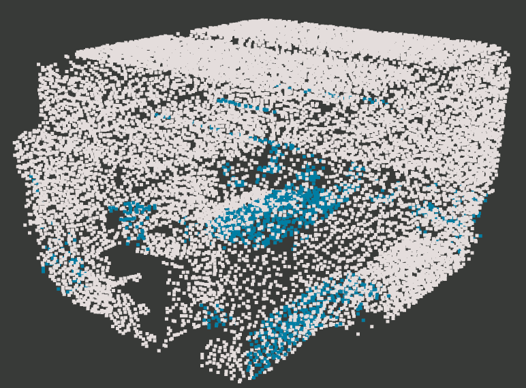
\includegraphics[width=0.45\textwidth]{figures/conf1 b 200 0.png}}  \label{fig:conf1 b 200 0} \hfill
    \subfigure[Semantic]{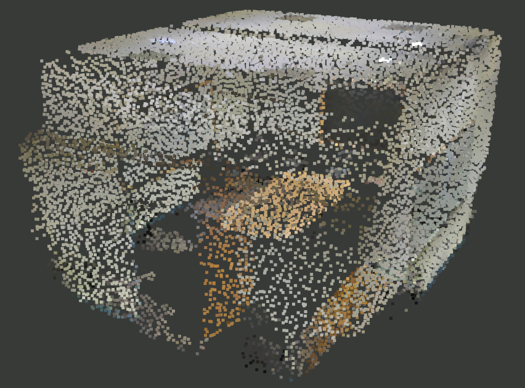
\includegraphics[width=0.45\textwidth]{figures/conf1 s 200 0.png}} \label{fig:conf1 s 200 0}
    \caption{Estimated Boundary and Semantics of Conference Room 1 with Viewpoint Pattern 1}
    \label{fig:conf1 0}
\end{figure}

\begin{figure}[H]
    \centering
    \subfigure[Boundary]{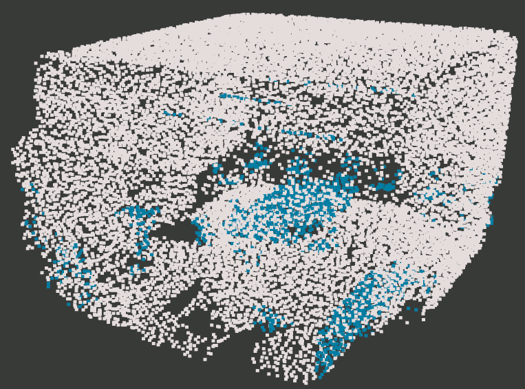
\includegraphics[width=0.45\textwidth]{figures/conf1 b 200 4.png}}  \label{fig:conf1 b 200 4} \hfill
    \subfigure[Semantic]{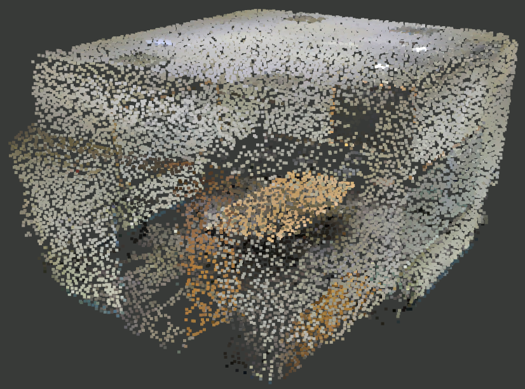
\includegraphics[width=0.45\textwidth]{figures/conf1 s 200 4.png}} \label{fig:conf1 s 200 4}
    \caption{Estimated Boundary and Semantics of Conference Room 1 with Viewpoint Pattern 2}
    \label{fig:conf1 4}
\end{figure}

\begin{figure}[H]
    \centering
    \subfigure[Boundary]{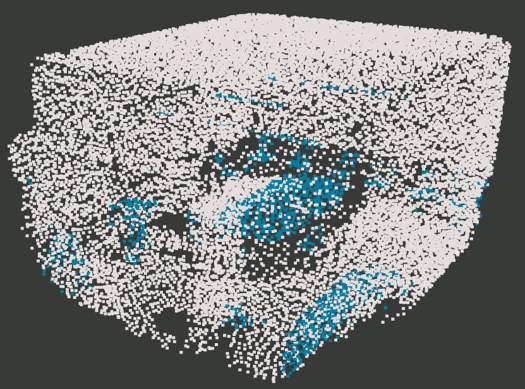
\includegraphics[width=0.45\textwidth]{figures/conf1 b 200 5.png}}  \label{fig:conf1 b 200 5} \hfill
    \subfigure[Semantic]{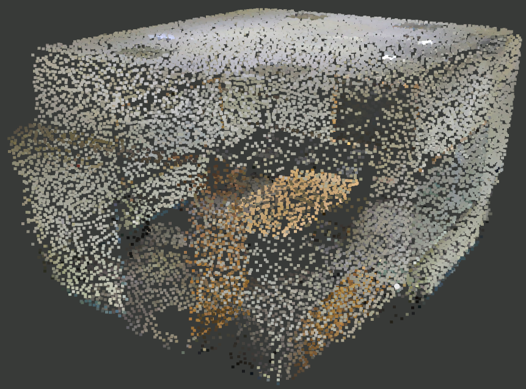
\includegraphics[width=0.45\textwidth]{figures/conf1 s 200 5.png}} \label{fig:conf1 s 200 5}
    \caption{Estimated Boundary and Semantics of Conference Room 1 with Viewpoint Pattern 3}
    \label{fig:conf1 5}
\end{figure}

\begin{figure}[H]
    \centering
    \subfigure[Boundary]{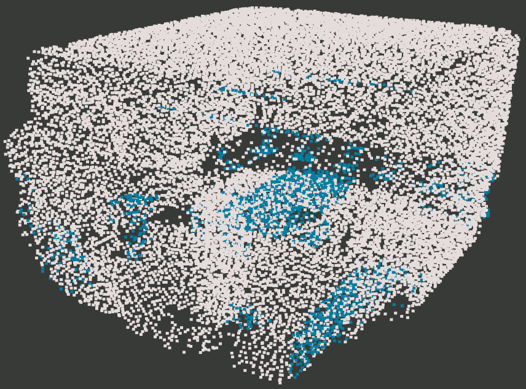
\includegraphics[width=0.45\textwidth]{figures/conf1 b 200 6.png}}  \label{fig:conf1 b 200 6} \hfill
    \subfigure[Semantic]{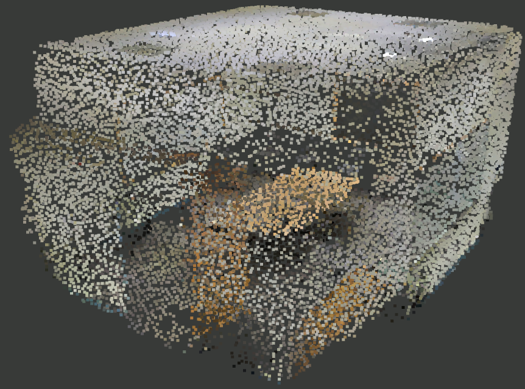
\includegraphics[width=0.45\textwidth]{figures/conf1 s 200 6.png}} \label{fig:conf1 s 200 6}
    \caption{Estimated Boundary and Semantics of Conference Room 1 with Viewpoint Pattern 4}
    \label{fig:conf1 6}
\end{figure}

\begin{table}[H]
    \centering
    \begin{tabular}{|c|c|c|}
        \hline
        \textbf{Pattern} & \textbf{Occluded Area Ratio} & \textbf{Boundary Ray Ratio} \\
        \hline
        1 & 0.291 & 0.271 \\
        2 & 0.108 & 0.172 \\
		3 & 0.153 & 0.211 \\
		4 & 0.071 & 0.165 \\
        \hline
    \end{tabular}
    \caption{Result of Conference Room 1}
    \label{tab:result of conference room 1}
\end{table}

The result shows that as the number of viewpoints increase, the \textit{Occluded Area Ratio} decrease. There are 2 viewpoints in both pattern 2 and 3, thus the increase of data in pattern 3 is not against our conclusion. Values of \textit{Boundary Ray Ratio} describe the same tendency, and they do not differ too much from data in \textit{Occluded Area Ratio}. Therefore, based on the result we consider \textit{Boundary Ray Ratio} as a reliable metric to represent the occlusion level of the scene presented by point cloud \textit{Conference Room 1}.       

\begin{figure}[H]
    \centering
    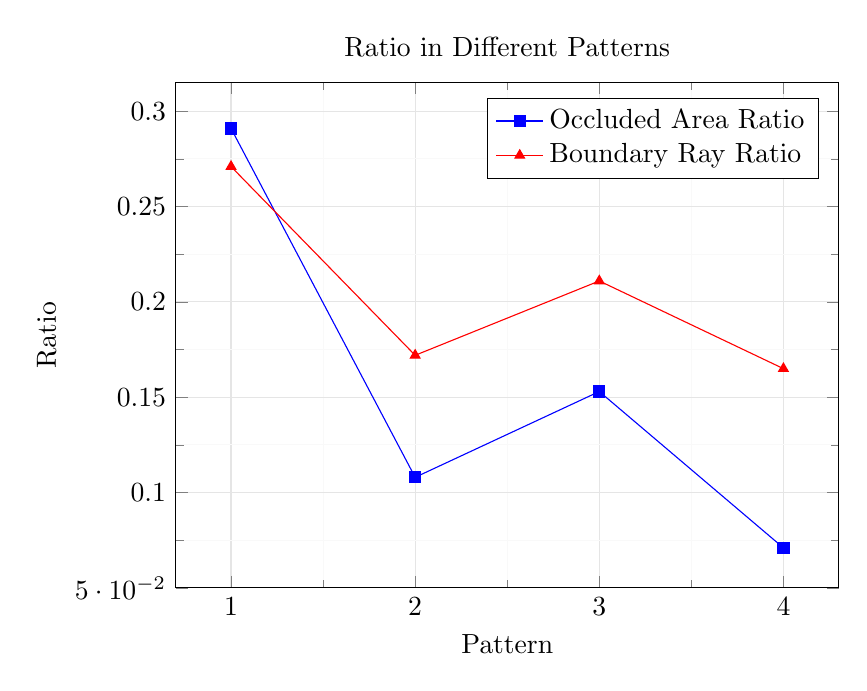
\begin{tikzpicture}
        \begin{axis}[
            title={Ratio in Different Patterns},
            xlabel={Pattern},
            ylabel={Ratio},
            grid=both,
            minor tick num=1,
            major grid style={lightgray},
            minor grid style={lightgray!25},
            legend pos=north east,
            legend style={cells={anchor=west}},
            xtick=data,  % Only show integer values on the x axis
            xticklabels={1,2,3,4},  % Specify the labels for the x axis
            ymin=0.05,
            width=10cm,
            height=8cm
        ]
        
        % Occluded Area Ratio Line
        \addplot[color=blue,mark=square*] coordinates {
            (1, 0.291)
            (2, 0.108)
            (3, 0.153)
            (4, 0.071)
        };
        \addlegendentry{Occluded Area Ratio}
        
        % Boundary Ray Ratio Line
        \addplot[color=red,mark=triangle*] coordinates {
            (1, 0.271)
            (2, 0.172)
            (3, 0.211)
            (4, 0.165)
        };
        \addlegendentry{Boundary Ray Ratio}

        \end{axis}
    \end{tikzpicture}
    \caption{Result of Conference Room 1}
    \label{fig:result of conference room 1}
\end{figure}

\paragraph{Conference Room 2}

We present the visualization of the scene \textit{Conference Room 2} in each step as explained in \ref{par:conf1 result}. Result is shown in Table \ref{tab:result of conference room 2} and Figure \ref{fig:result of conference room 2}.

\vspace{10pt}

\begin{figure}[H]
    \centering
    \includegraphics*[width=1.0\textwidth]{figures/estimate conf2.png}
    \caption{Estimate Mesh from Conference Room 2}
    \label{fig:estimate mesh from conference room 2}
\end{figure}

\begin{figure}[H]
    \centering
    \subfigure[Boundary]{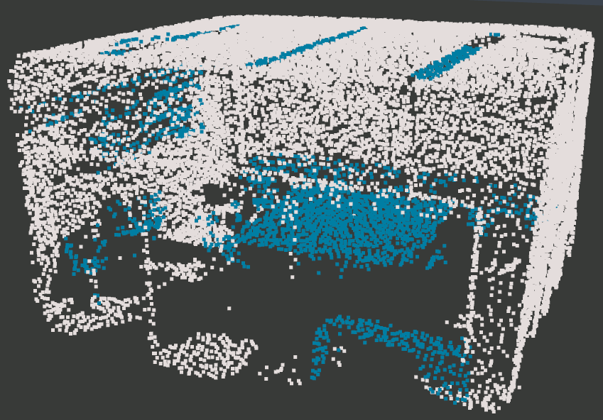
\includegraphics[width=0.45\textwidth]{figures/conf2 b 200 0.png}}  \label{fig:conf2 b 200 0} \hfill
    \subfigure[Semantic]{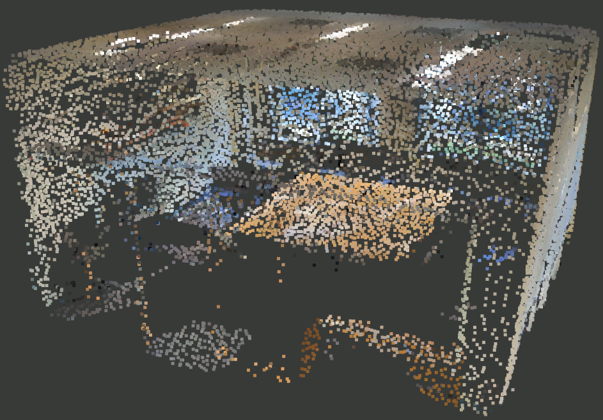
\includegraphics[width=0.45\textwidth]{figures/conf2 s 200 0.png}} \label{fig:conf2 s 200 0}
    \caption{Estimated Boundary and Semantics of Conference Room 2 with Viewpoint Pattern 1}
    \label{fig:conf2 0}
\end{figure}

\begin{figure}[H]
    \centering
    \subfigure[Boundary]{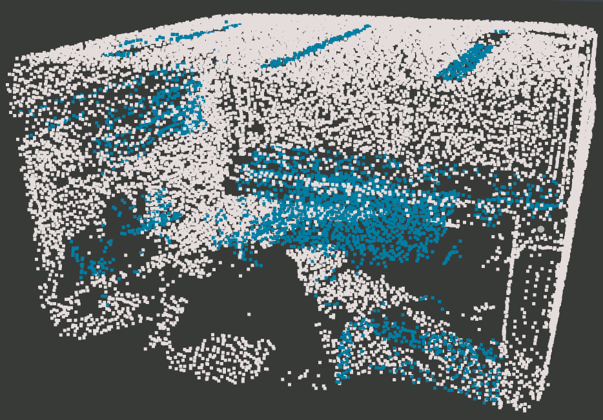
\includegraphics[width=0.45\textwidth]{figures/conf2 b 200 4.png}}  \label{fig:conf2 b 200 4} \hfill
    \subfigure[Semantic]{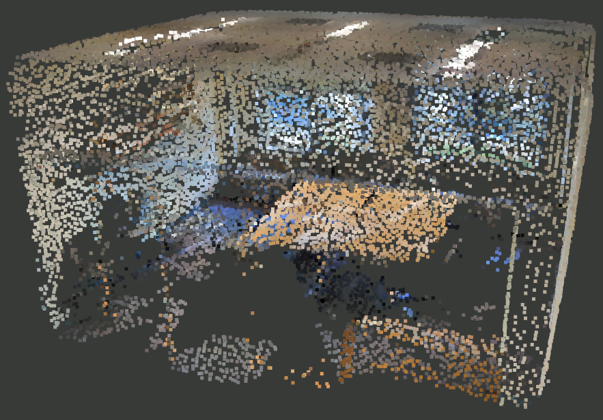
\includegraphics[width=0.45\textwidth]{figures/conf2 s 200 4.png}} \label{fig:conf2 s 200 4}
    \caption{Estimated Boundary and Semantics of Conference Room 2 with Viewpoint Pattern 2}
    \label{fig:conf2 4}
\end{figure}

\begin{figure}[H]
    \centering
    \subfigure[Boundary]{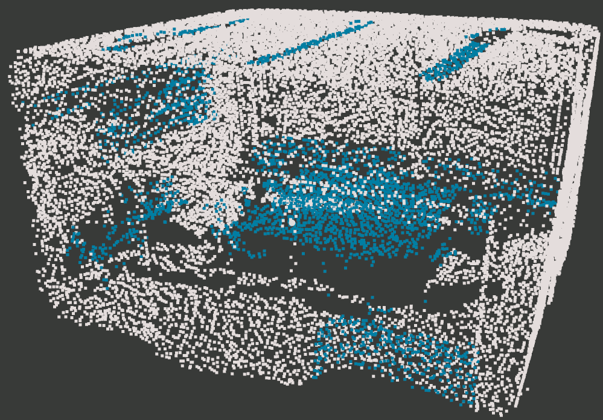
\includegraphics[width=0.45\textwidth]{figures/conf2 b 200 5.png}}  \label{fig:conf2 b 200 5} \hfill
    \subfigure[Semantic]{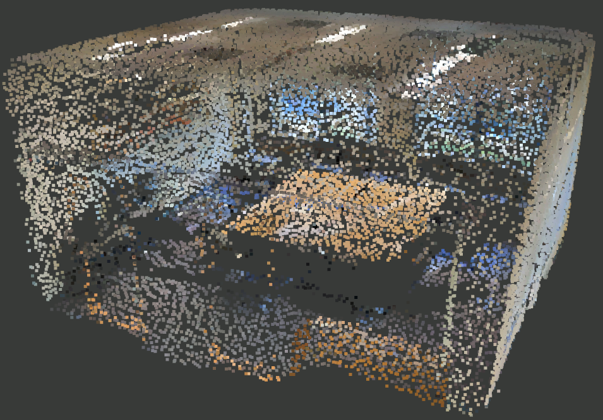
\includegraphics[width=0.45\textwidth]{figures/conf2 s 200 5.png}} \label{fig:conf2 s 200 5}
    \caption{Estimated Boundary and Semantics of Conference Room 2 with Viewpoint Pattern 3}
    \label{fig:conf2 5}
\end{figure}

\begin{figure}[H]
    \centering
    \subfigure[Boundary]{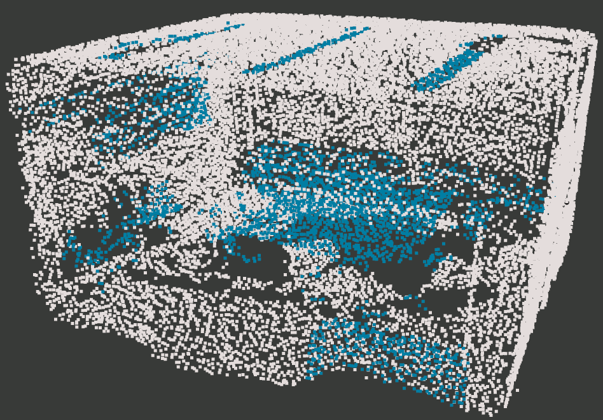
\includegraphics[width=0.45\textwidth]{figures/conf2 b 200 6.png}}  \label{fig:conf2 b 200 6} \hfill
    \subfigure[Semantic]{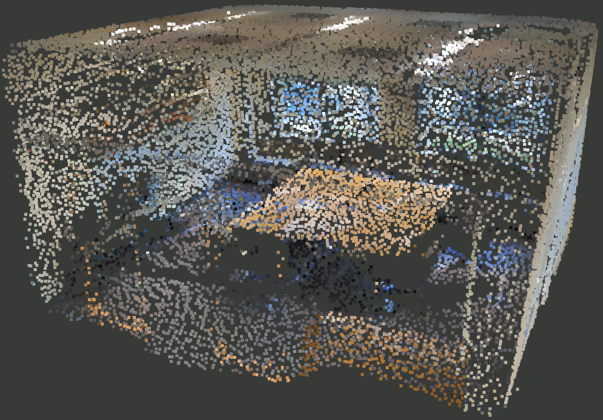
\includegraphics[width=0.45\textwidth]{figures/conf2 s 200 6.png}} \label{fig:conf2 s 200 6}
    \caption{Estimated Boundary and Semantics of Conference Room 2 with Viewpoint Pattern 4}
    \label{fig:conf2 6}
\end{figure}

\begin{table}[H]
    \centering
    \begin{tabular}{|c|c|c|}
        \hline
        \textbf{Pattern} & \textbf{Occluded Area Ratio} & \textbf{Boundary Ray Ratio} \\
        \hline
        1 & 0.371 & 0.329 \\
        2 & 0.294 & 0.258 \\
		3 & 0.264 & 0.255 \\
		4 & 0.218 & 0.224 \\
        \hline
    \end{tabular}
    \caption{Result of Conference Room 2}
    \label{tab:result of conference room 2}
\end{table}

Both ratios display the same trend, thus we can conclude that \textit{Boundary Ray Ratio} is able to assess the occlusion level of \textit{Conference Room 2}.

\begin{figure}[H]
    \centering
    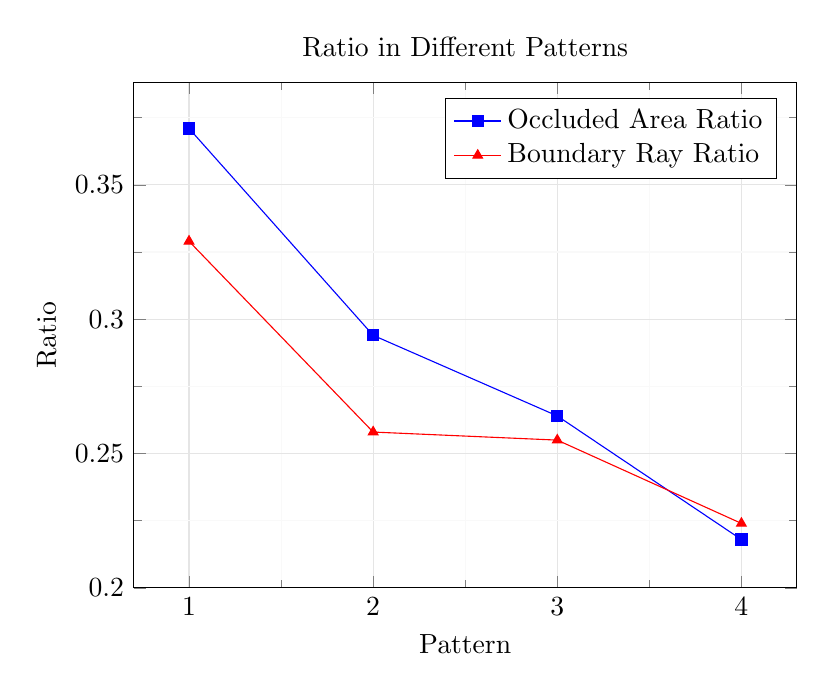
\begin{tikzpicture}
        \begin{axis}[
            title={Ratio in Different Patterns},
            xlabel={Pattern},
            ylabel={Ratio},
            grid=both,
            minor tick num=1,
            major grid style={lightgray},
            minor grid style={lightgray!25},
            legend pos=north east,
            legend style={cells={anchor=west}},
            xtick=data,  % Only show integer values on the x axis
            xticklabels={1,2,3,4},  % Specify the labels for the x axis
            ymin=0.2,
            width=10cm,
            height=8cm
        ]
        
        % Occluded Area Ratio Line
        \addplot[color=blue,mark=square*] coordinates {
            (1, 0.371)
            (2, 0.294)
            (3, 0.264)
            (4, 0.218)
        };
        \addlegendentry{Occluded Area Ratio}
        
        % Boundary Ray Ratio Line
        \addplot[color=red,mark=triangle*] coordinates {
            (1, 0.329)
            (2, 0.258)
            (3, 0.255)
            (4, 0.224)
        };
        \addlegendentry{Boundary Ray Ratio}

        \end{axis}
    \end{tikzpicture}
    \caption{Result of Conference Room 2}
    \label{fig:result of conference room 2}
\end{figure}

\vspace{30pt}

\paragraph{Copy Room}

We follow the same workflow as shown before to present the visualization of the scene \textit{Copy Room} in each step. Result is shown in Table \ref{tab:result of copy room} and Figure \ref{fig:result of copy room}.

\vspace{30pt}

\begin{figure}[H]
    \centering
    \includegraphics*[width=1.0\textwidth, height=0.4\textwidth]{figures/estimate copy.png}
    \caption{Estimate Mesh from Copy Room}
    \label{fig:estimate mesh from copy room}
\end{figure}

\begin{figure}[H]
    \centering
    \subfigure[Boundary]{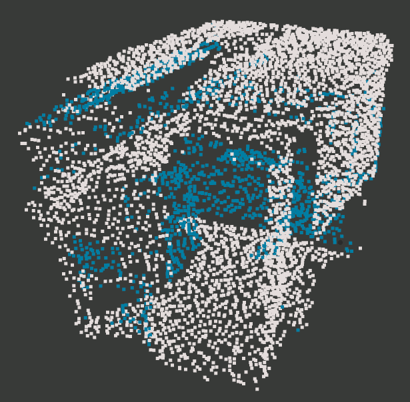
\includegraphics[width=0.37\textwidth, height=0.33\textwidth]{figures/copy b 200 0.png}}  \label{fig:copy b 200 0} \hfill
    \subfigure[Semantic]{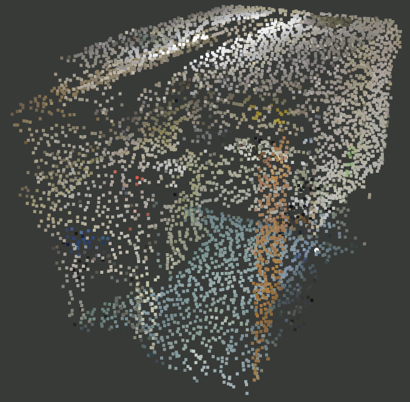
\includegraphics[width=0.37\textwidth, height=0.33\textwidth]{figures/copy s 200 0.png}} \label{fig:copy s 200 0}
    \caption{Estimated Boundary and Semantics of Copy Room with Viewpoint Pattern 1}
    \label{fig:copy 0}
\end{figure}

\begin{figure}[H]
    \centering
    \subfigure[Boundary]{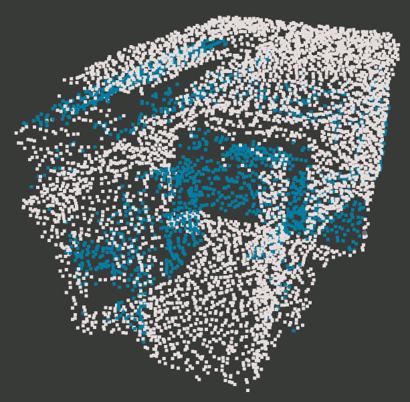
\includegraphics[width=0.37\textwidth, height=0.33\textwidth]{figures/copy b 200 4.png}}  \label{fig:copy b 200 4} \hfill
    \subfigure[Semantic]{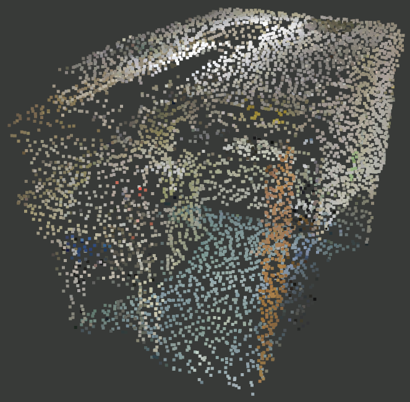
\includegraphics[width=0.37\textwidth, height=0.33\textwidth]{figures/copy s 200 4.png}} \label{fig:copy s 200 4}
    \caption{Estimated Boundary and Semantics of Copy Room with Viewpoint Pattern 2}
    \label{fig:copy 4}
\end{figure}

\begin{figure}[H]
    \centering
    \subfigure[Boundary]{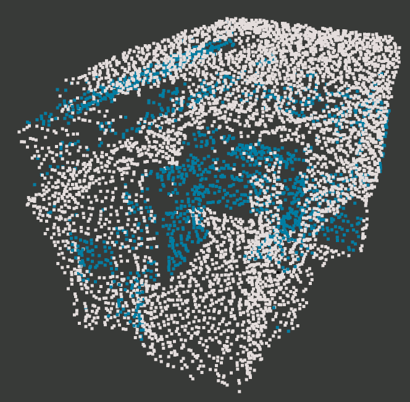
\includegraphics[width=0.37\textwidth, height=0.33\textwidth]{figures/copy b 200 5.png}}  \label{fig:copy b 200 5} \hfill
    \subfigure[Semantic]{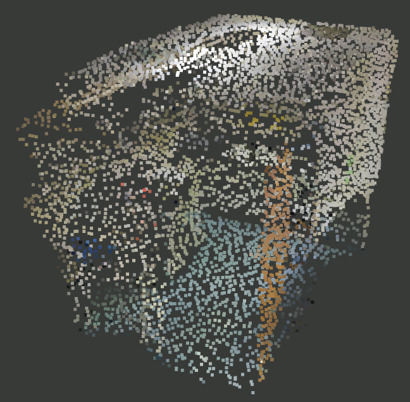
\includegraphics[width=0.37\textwidth, height=0.33\textwidth]{figures/copy s 200 5.png}} \label{fig:copy s 200 5}
    \caption{Estimated Boundary and Semantics of Copy Room with Viewpoint Pattern 3}
    \label{fig:copy 5}
\end{figure}

\begin{figure}[H]
    \centering
    \subfigure[Boundary]{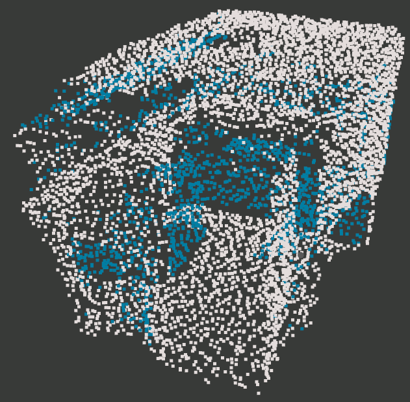
\includegraphics[width=0.37\textwidth, height=0.33\textwidth]{figures/copy b 200 6.png}}  \label{fig:copy b 200 6} \hfill
    \subfigure[Semantic]{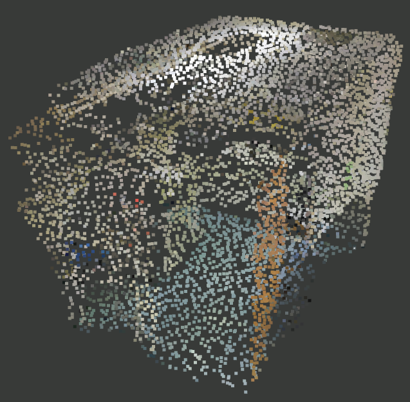
\includegraphics[width=0.37\textwidth, height=0.33\textwidth]{figures/copy s 200 6.png}} \label{fig:copy s 200 6}
    \caption{Estimated Boundary and Semantics of Copy Room with Viewpoint Pattern 4}
    \label{fig:copy 6}
\end{figure}

\begin{table}[H]
    \centering
    \begin{tabular}{|c|c|c|}
        \hline
        \textbf{Pattern} & \textbf{Occluded Area Ratio} & \textbf{Boundary Ray Ratio} \\
        \hline
        1 & 0.156 & 0.366 \\
        2 & 0.090 & 0.343 \\
		3 & 0.070 & 0.337 \\
		4 & 0.040 & 0.331 \\
        \hline
    \end{tabular}
    \caption{Result of Copy Room}
    \label{tab:result of copy room}
\end{table}

Although the result between 2 ratios has more difference than the data presented in previous experiments, it shows the same trend as we change pattern of viewpoint again. Hence, we think that \textit{Boundary Ray Ratio} can still represent the occlusion level of \textit{Copy Room}. 

\begin{figure}[H]
    \centering
    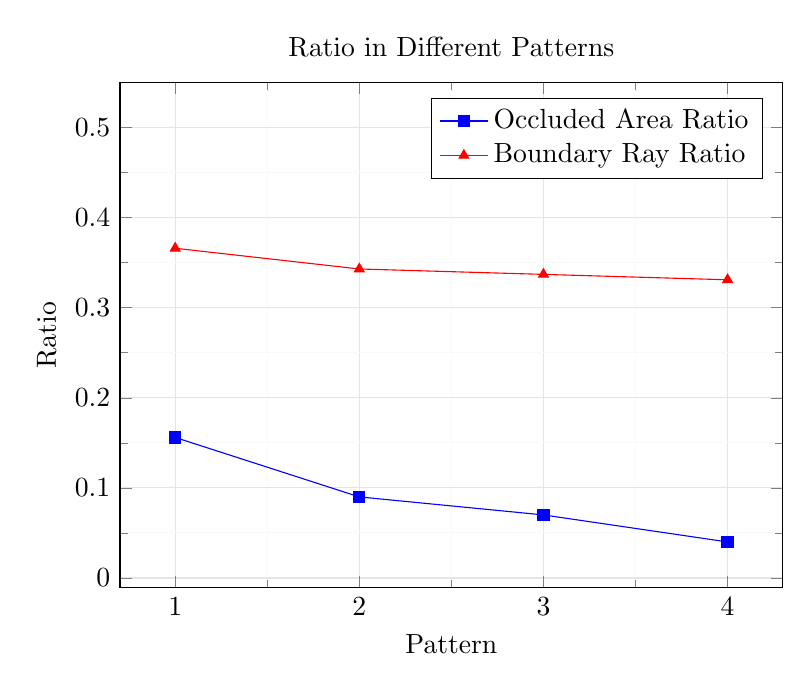
\begin{tikzpicture}
        \begin{axis}[
            title={Ratio in Different Patterns},
            xlabel={Pattern},
            ylabel={Ratio},
            grid=both,
            minor tick num=1,
            major grid style={lightgray},
            minor grid style={lightgray!25},
            legend pos=north east,
            legend style={cells={anchor=west}},
            xtick=data,  % Only show integer values on the x axis
            xticklabels={1,2,3,4},  % Specify the labels for the x axis
            ymax=0.55,
            width=10cm,
            height=8cm
        ]
        
        % Occluded Area Ratio Line
        \addplot[color=blue,mark=square*] coordinates {
            (1, 0.156)
            (2, 0.090)
            (3, 0.070)
            (4, 0.040)
        };
        \addlegendentry{Occluded Area Ratio}
        
        % Boundary Ray Ratio Line
        \addplot[color=red,mark=triangle*] coordinates {
            (1, 0.366)
            (2, 0.343)
            (3, 0.337)
            (4, 0.331)
        };
        \addlegendentry{Boundary Ray Ratio}

        \end{axis}
    \end{tikzpicture}
    \caption{Result of Copy Room}
    \label{fig:result of copy room}
\end{figure}

In this section we conducted 3 experiments to compute and compare occlusion level for different scenes. The result proves that \textit{Boundary Ray Ratio} can be applied for computation in subsequent experiments.

\section{Correlation}

The major task in this part is to find correlation between occlusion level and performance of segmentation. We use the same input data as in previous section. Due to the difference in terms of complexity and structure of the 3 scenes, it's obviously not a proper way to directly compare the metrics of them. Thus, the first step here is to create a set of occluded point clouds for each room and compute occlusion level for each of them. After the generation, we use \textit{Minkowski Engine} for semantic segmentation. In the final step, we calculate evaluation metrics for each occluded cloud which is generated under different pattern of light sources. With occlusion level and result of evaluation metrics of this data set, we may correlate them and analyze the impact of occlusion on semantic segmentation. The comparison should be done between data generated from the same scene.

\subsection{Setup}

To generate occluded point cloud, we place spherical light sources in different locations of the scene. Each light source cast a set of rays based on the result of halton sampling on its surface. We will then record the point hit by rays for the first time to generate occluded point cloud.

\vspace{10pt}

We apply the same pattern of placement illustrated in Figure \ref{fig:pattern of viewpoints} to place our sphere lights in the scene. We sample 20 thousands points on each sphere and we thus generate 20 thousands rays per spherical light source.

\vspace{10pt}

Data with semantic information is then generated for each occluded point cloud via \textit{Minkowski Engine}. We calculate values of evaluation metrics in a pair-wise manner.


\subsection{Results}

In this part, we display visualization for each pair of clouds which includes one occluded cloud with ground truth RGB information and one cloud with semantic label represented by specific colors. In the end of each part, output of the computational pipeline will be shown in tables and graphs where we can compare data more conveniently.

\paragraph{Conference Room 1}

We first exhibit visual output of generated point cloud and corresponding segmentation of \textit{Conference Room 1}.

\begin{figure}[H]
    \centering
    \subfigure[Occluded Cloud]{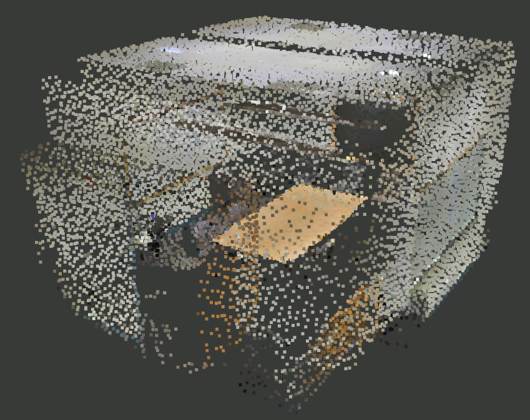
\includegraphics[width=0.42\textwidth]{figures/conf1 0.png}}  \label{fig:conf1 0 occluded} \hfill
    \subfigure[Segmentation]{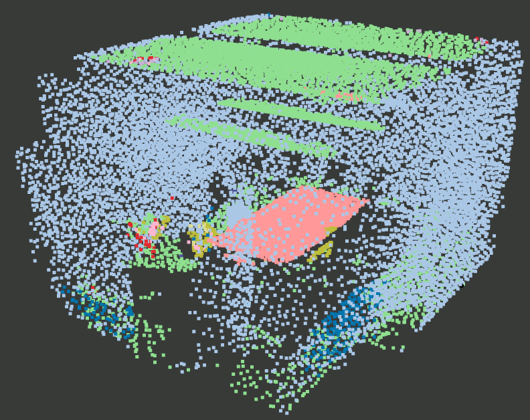
\includegraphics[width=0.42\textwidth]{figures/conf1 0 seg.png}} \label{fig:conf1 0 seg}
    \caption{Occluded Cloud and Corresponding Segmentation under Light Pattern 1 of Conference Room 1}
    \label{fig:conf1 0 occ and seg}
\end{figure}

\begin{figure}[H]
    \centering
    \subfigure[Occluded Cloud]{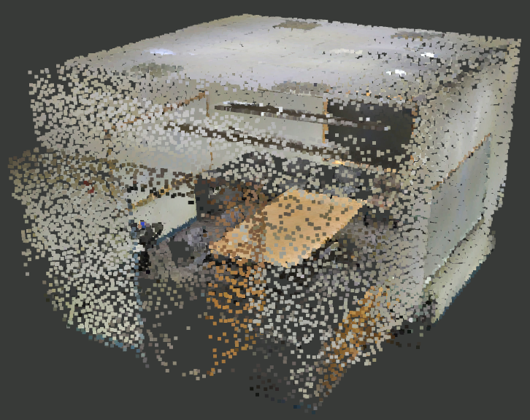
\includegraphics[width=0.42\textwidth]{figures/conf1 4.png}}  \label{fig:conf1 4 occluded} \hfill
    \subfigure[Segmentation]{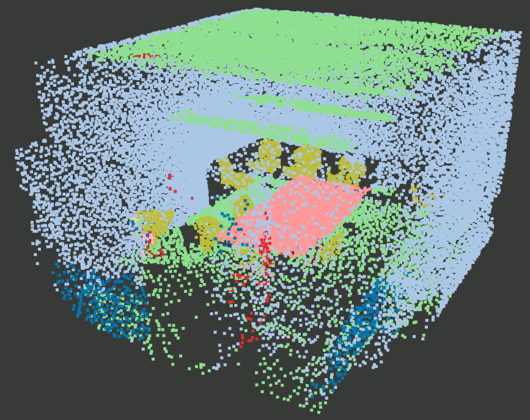
\includegraphics[width=0.42\textwidth]{figures/conf1 4 seg.png}} \label{fig:conf1 4 seg}
    \caption{Occluded Cloud and Corresponding Segmentation under Light Pattern 2 of Conference Room 1}
    \label{fig:conf1 4 occ and seg}
\end{figure}

\begin{figure}[H]
    \centering
    \subfigure[Occluded Cloud]{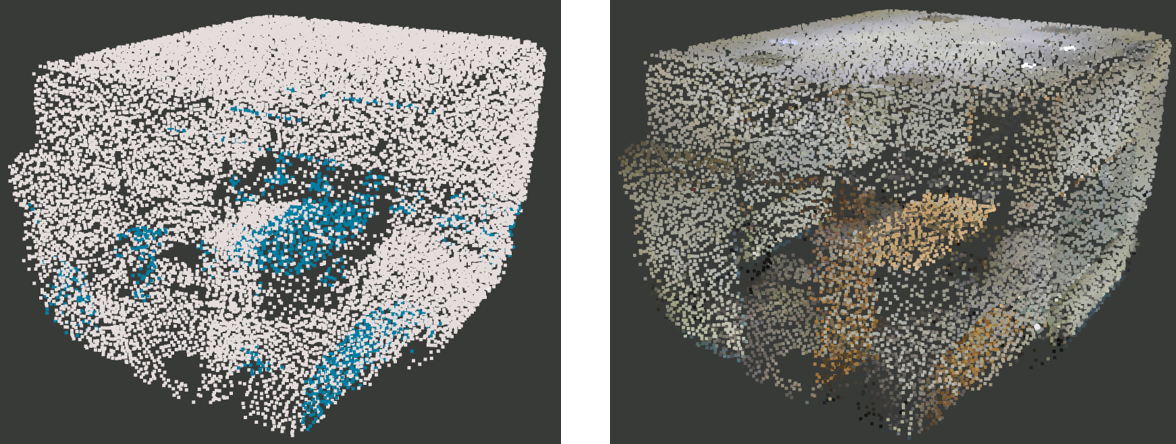
\includegraphics[width=0.42\textwidth]{figures/conf1 5.png}}  \label{fig:conf1 5 occluded} \hfill
    \subfigure[Segmentation]{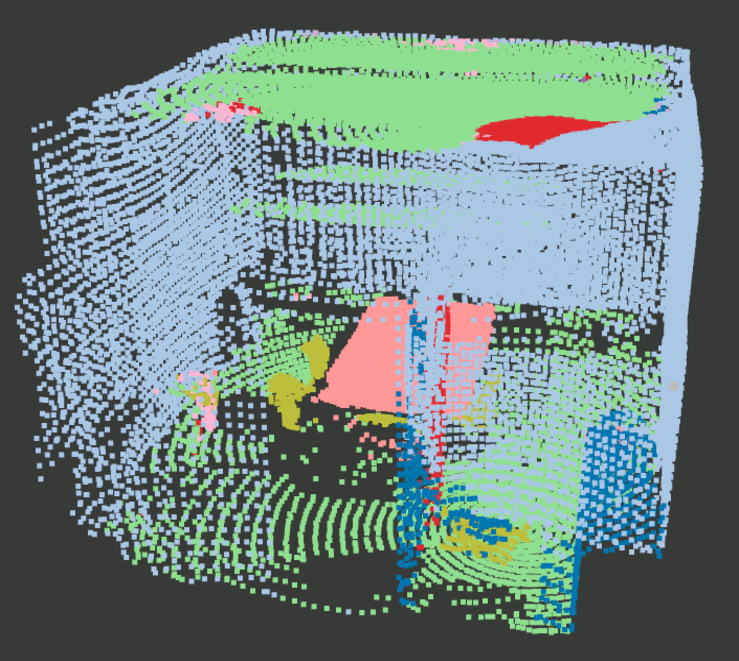
\includegraphics[width=0.42\textwidth]{figures/conf1 5 seg.png}} \label{fig:conf1 5 seg}
    \caption{Occluded Cloud and Corresponding Segmentation under Light Pattern 3 of Conference Room 1}
    \label{fig:conf1 5 occ and seg}
\end{figure}

\begin{figure}[H]
    \centering
    \subfigure[Occluded Cloud]{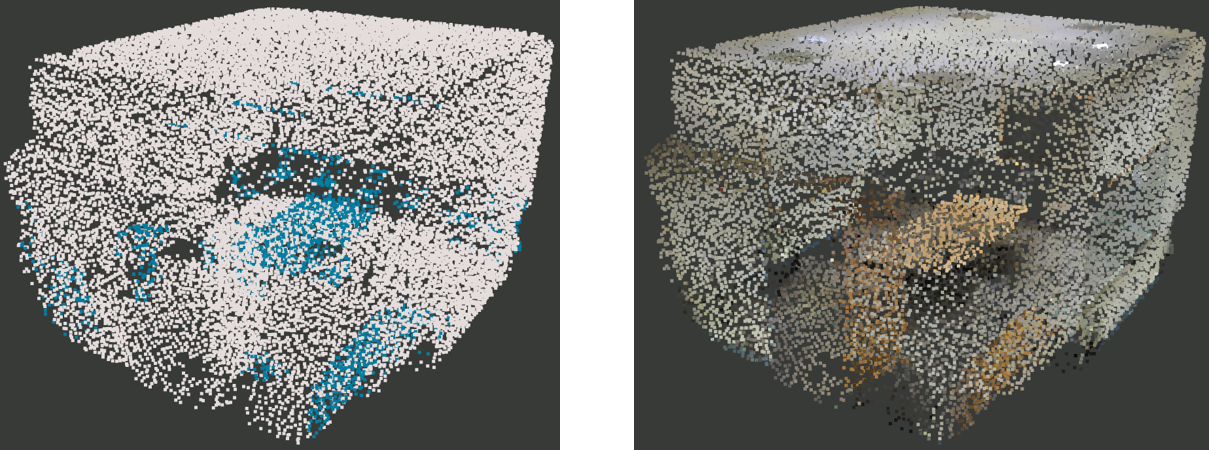
\includegraphics[width=0.42\textwidth]{figures/conf1 6.png}}  \label{fig:conf1 6 occluded} \hfill
    \subfigure[Segmentation]{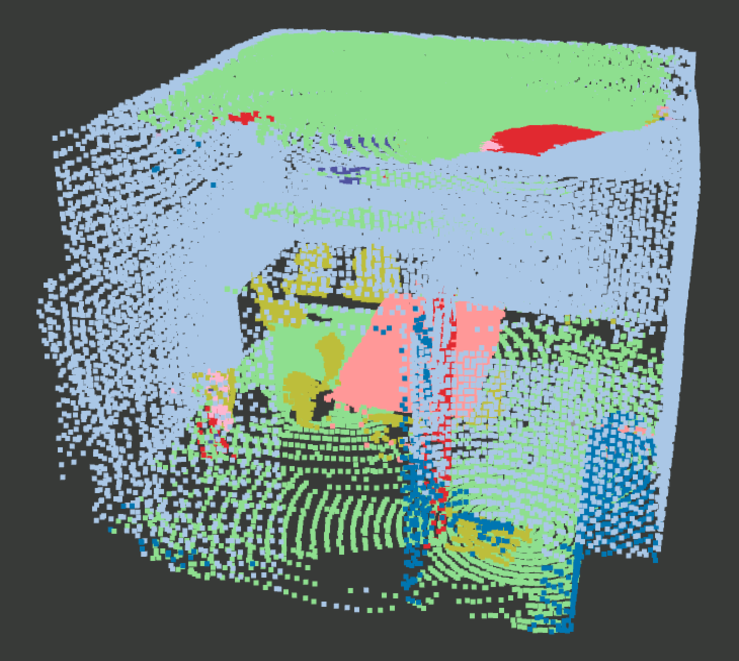
\includegraphics[width=0.42\textwidth]{figures/conf1 6 seg.png}} \label{fig:conf1 6 seg}
    \caption{Occluded Cloud and Corresponding Segmentation under Light Pattern 4 of Conference Room 1}
    \label{fig:conf1 6 occ and seg}
\end{figure}

The result is shown in Table \ref{tab:evaluation metrics of conference room 1} and Figure \ref{fig:evaluation metrics of conference room 1}.

\begin{table}[H]
    \centering
    \begin{tabular}{|c|c|c|c|c|c|c|}
        \hline
        Pattern & Occlusion & Accuracy & IoU & Precision & Recall & F1 Score \\
        \hline
        1 & 0.241 & 0.893 & 0.497 & 0.652 & 0.675 & 0.664 \\
        2 & 0.168 & 0.912 & 0.585 & 0.736 & 0.741 & 0.738 \\
        3 & 0.197 & 0.878 & 0.461 & 0.655 & 0.609 & 0.631 \\
        4 & 0.161 & 0.894 & 0.524 & 0.707 & 0.669 & 0.687 \\
        \hline
    \end{tabular}
    \caption{Evaluation Metrics of Conference Room 1}
    \label{tab:evaluation metrics of conference room 1}
\end{table}

\vspace{20pt}

From the graph it's obvious that occlusion level is inversely related to these metrics.

\begin{figure}[H]
    \centering
    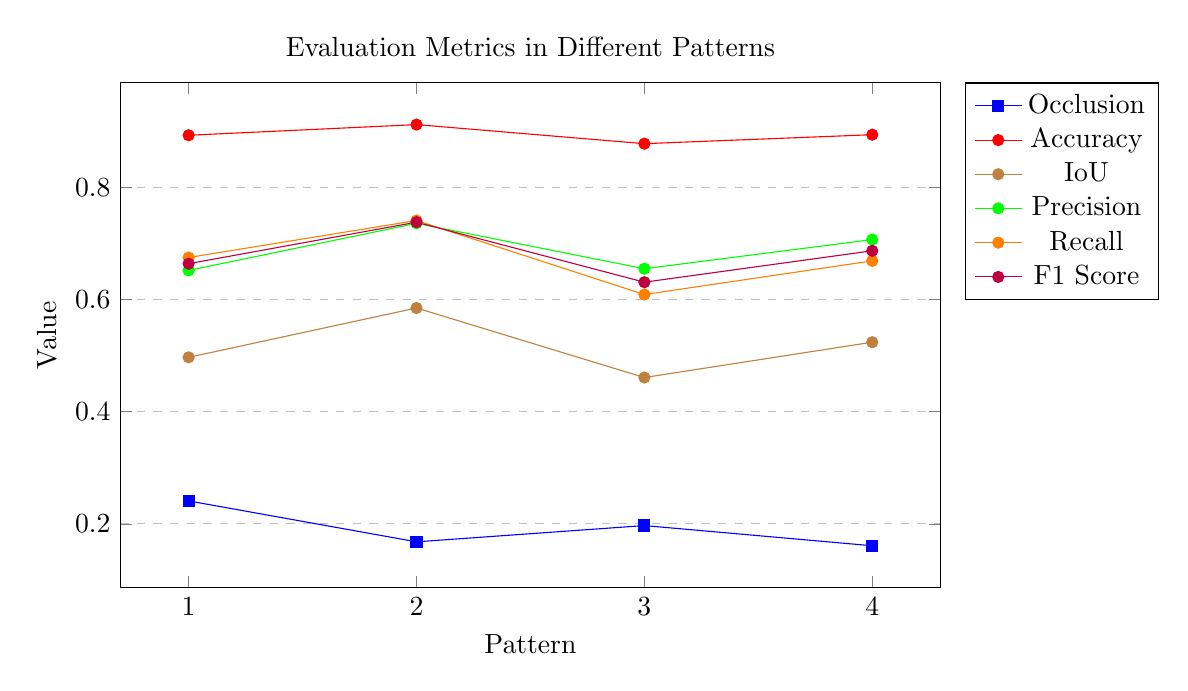
\begin{tikzpicture}
    \begin{axis}[
        title={Evaluation Metrics in Different Patterns},
        xlabel={Pattern},
        ylabel={Value},
        legend pos=outer north east,
        ymajorgrids=true,
        grid style=dashed,
        xtick=data,
        symbolic x coords={1,2,3,4},
        width=12cm,
        height=8cm,
    ]
    
    \addplot[mark=square*,blue] coordinates {
        (1, 0.241)
        (2, 0.168)
        (3, 0.197)
        (4, 0.161)
    };
    \addlegendentry{Occlusion}
    
    \addplot[mark=*,red] coordinates {
        (1, 0.893)
        (2, 0.912)
        (3, 0.878)
        (4, 0.894)
    };
    \addlegendentry{Accuracy}
    
    \addplot[mark=*,brown] coordinates {
        (1, 0.497)
        (2, 0.585)
        (3, 0.461)
        (4, 0.524)
    };
    \addlegendentry{IoU}
    
    \addplot[mark=*,green] coordinates {
        (1, 0.652)
        (2, 0.736)
        (3, 0.655)
        (4, 0.707)
    };
    \addlegendentry{Precision}
    
    \addplot[mark=*,orange] coordinates {
        (1, 0.675)
        (2, 0.741)
        (3, 0.609)
        (4, 0.669)
    };
    \addlegendentry{Recall}
    
    \addplot[mark=*,purple] coordinates {
        (1, 0.664)
        (2, 0.738)
        (3, 0.631)
        (4, 0.687)
    };
    \addlegendentry{F1 Score}
    
    \end{axis}
    \end{tikzpicture}
    \caption{Evaluation Metrics of Conference Room 1}
    \label{fig:evaluation metrics of conference room 1}
\end{figure}


\paragraph{Conference Room 2}

Same workflow here to present our results.

\begin{figure}[H]
    \centering
    \subfigure[Occluded Cloud]{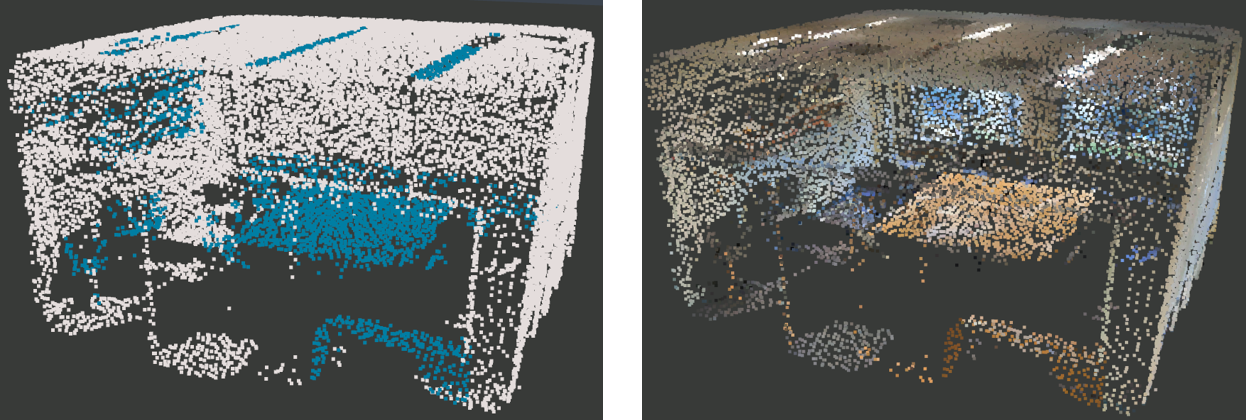
\includegraphics[width=0.45\textwidth]{figures/conf2 0.png}}  \label{fig:conf2 0 occluded} \hfill
    \subfigure[Segmentation]{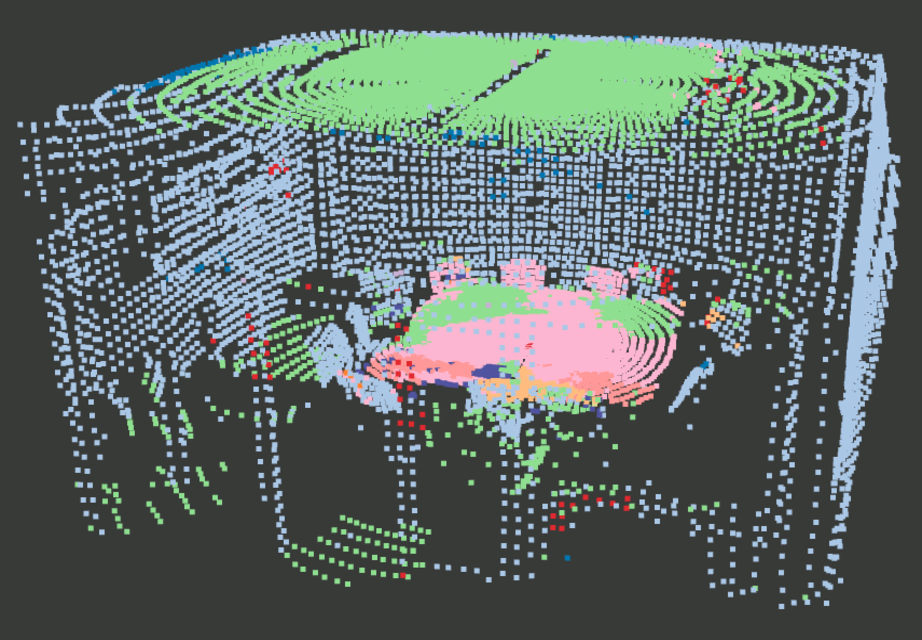
\includegraphics[width=0.45\textwidth]{figures/conf2 0 seg.png}} \label{fig:conf2 0 seg}
    \caption{Occluded Cloud and Corresponding Segmentation under Light Pattern 1 of Conference Room 2}
    \label{fig:conf2 0 occ and seg}
\end{figure}

\begin{figure}[H]
    \centering
    \subfigure[Occluded Cloud]{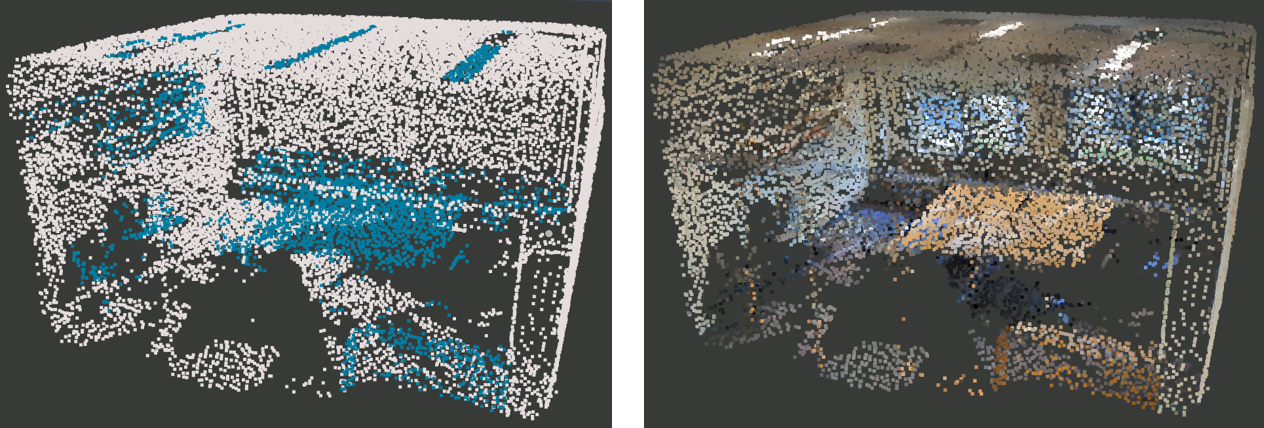
\includegraphics[width=0.45\textwidth]{figures/conf2 4.png}}  \label{fig:conf2 4 occluded} \hfill
    \subfigure[Segmentation]{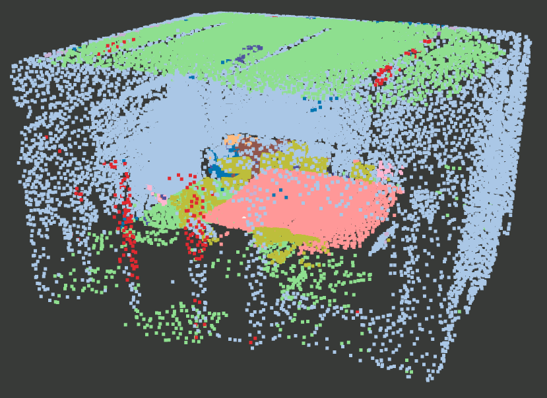
\includegraphics[width=0.45\textwidth]{figures/conf2 4 seg.png}} \label{fig:conf2 4 seg}
    \caption{Occluded Cloud and Corresponding Segmentation  under Light Pattern 2 of Conference Room 2}
    \label{fig:conf2 4 occ and seg}
\end{figure}

\begin{figure}[H]
    \centering
    \subfigure[Occluded Cloud]{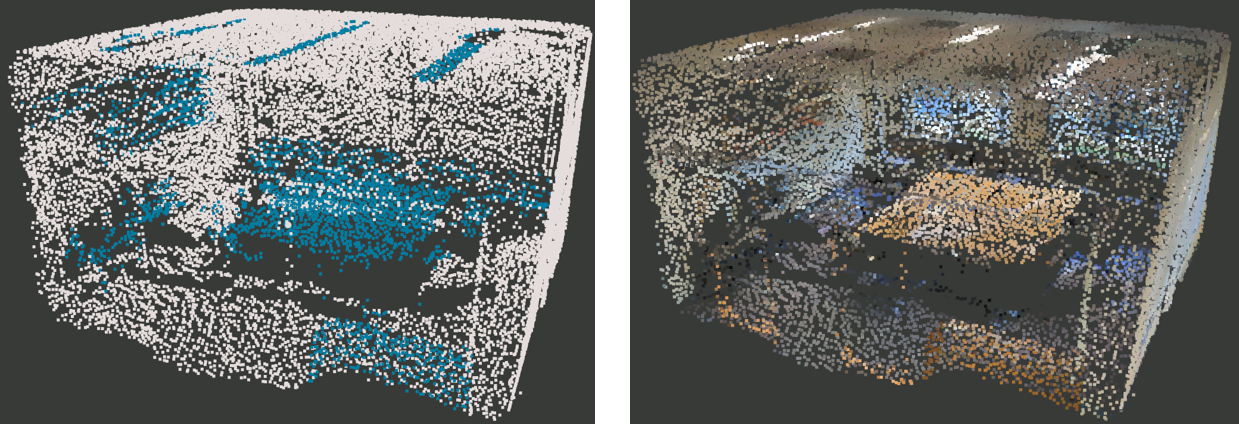
\includegraphics[width=0.45\textwidth]{figures/conf2 5.png}}  \label{fig:conf2 5 occluded} \hfill
    \subfigure[Segmentation]{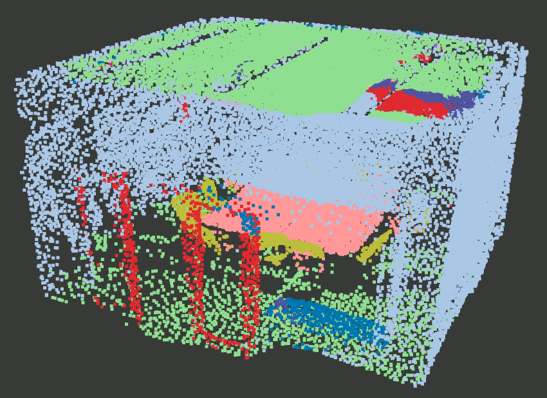
\includegraphics[width=0.45\textwidth]{figures/conf2 5 seg.png}} \label{fig:conf2 5 seg}
    \caption{Occluded Cloud and Corresponding Segmentation under Light Pattern 3 of Conference Room 2}
    \label{fig:conf2 5 occ and seg}
\end{figure}

\begin{figure}[H]
    \centering
    \subfigure[Occluded Cloud]{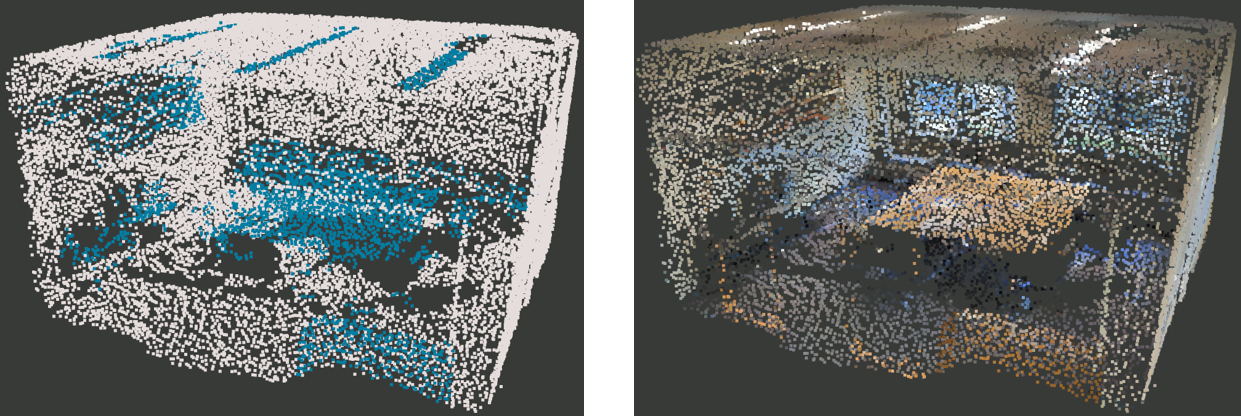
\includegraphics[width=0.45\textwidth]{figures/conf2 6.png}}  \label{fig:conf2 6 occluded} \hfill
    \subfigure[Segmentation]{\includegraphics[width=0.45\textwidth]{figures/conf2 6 seg.png}} \label{fig:conf2 6 seg}
    \caption{Occluded Cloud and Corresponding Segmentation under Light Pattern 4 of Conference Room 2}
    \label{fig:conf2 6 occ and seg}
\end{figure}

The result is shown in \ref{tab:evaluation metrics of conference room 2} and \ref{fig:evaluation metrics of conference room 2}.

\begin{table}[H]
    \centering
    \begin{tabular}{|c|c|c|c|c|c|c|}
        \hline
        Pattern & Occlusion & Accuracy & IoU & Precision & Recall & F1 Score \\
        \hline
        1 & 0.319 & 0.882 & 0.44 & 0.58 & 0.645 & 0.611 \\
        2 & 0.279 & 0.923 & 0.595 & 0.721 & 0.772 & 0.746 \\
        3 & 0.259 & 0.879 & 0.452 & 0.632 & 0.614 & 0.622 \\
        4 & 0.227 & 0.901 & 0.522 & 0.685 & 0.687 & 0.686 \\
        \hline
    \end{tabular}
    \caption{Evaluation Metrics of Conference Room 2}
    \label{tab:evaluation metrics of conference room 2}
\end{table}

\begin{figure}[H]
    \centering
    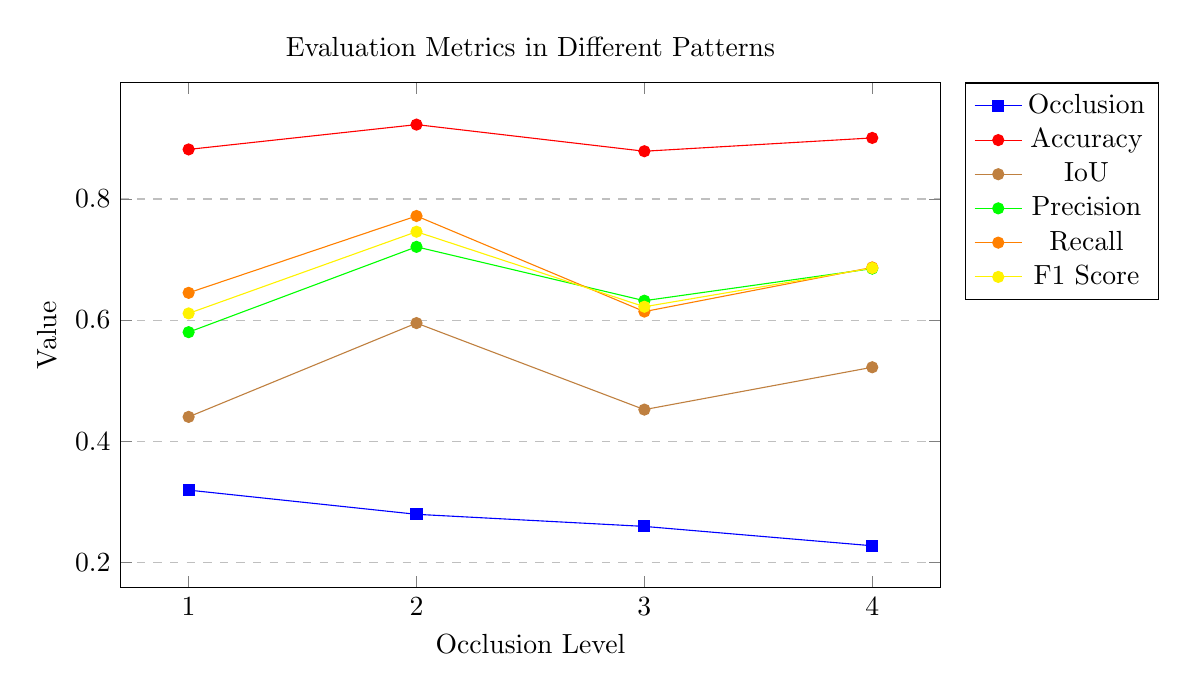
\begin{tikzpicture}
    \begin{axis}[
        title={Evaluation Metrics in Different Patterns},
        xlabel={Occlusion Level},
        ylabel={Value},
        legend pos=outer north east,
        ymajorgrids=true,
        grid style=dashed,
        xtick=data,
        symbolic x coords={1,2,3,4},
        width=12cm,
        height=8cm,
    ]
    
    \addplot[mark=square*,blue] coordinates {
        (1, 0.319)
        (2, 0.279)
        (3, 0.259)
        (4, 0.227)
    };
    \addlegendentry{Occlusion}
    
    \addplot[mark=*,red] coordinates {
        (1, 0.882)
        (2, 0.923)
        (3, 0.879)
        (4, 0.901)
    };
    \addlegendentry{Accuracy}
    
    \addplot[mark=*,brown] coordinates {
        (1, 0.44)
        (2, 0.595)
        (3, 0.452)
        (4, 0.522)
    };
    \addlegendentry{IoU}
    
    \addplot[mark=*,green] coordinates {
        (1, 0.58)
        (2, 0.721)
        (3, 0.632)
        (4, 0.685)
    };
    \addlegendentry{Precision}
    
    \addplot[mark=*,orange] coordinates {
        (1, 0.645)
        (2, 0.772)
        (3, 0.614)
        (4, 0.687)
    };
    \addlegendentry{Recall}

    \addplot[mark=*,yellow] coordinates {
        (1, 0.611)
        (2, 0.746)
        (3, 0.622)
        (4, 0.686)
    };
    \addlegendentry{F1 Score}
    
    \end{axis}
    \end{tikzpicture}
    \caption{Evaluation Metrics of Conference Room 2}
    \label{fig:evaluation metrics of conference room 2}
\end{figure}

\paragraph{Copy Room}

We show the resulting visualization first.

\begin{figure}[H]
    \centering
    \subfigure[Occluded Cloud]{\includegraphics[width=0.37\textwidth, height=0.33\textwidth]{figures/copy 0.png}}  \label{fig:copy 0 occluded} \hfill
    \subfigure[Segmentation]{\includegraphics[width=0.37\textwidth, height=0.33\textwidth]{figures/copy 0 seg.png}} \label{fig:copy 0 seg}
    \caption{Occluded Cloud and Corresponding Segmentation under Light Pattern 1 of Copy Room}
    \label{fig:copy 0 occ and seg}
\end{figure}

\begin{figure}[H]
    \centering
    \subfigure[Occluded Cloud]{\includegraphics[width=0.37\textwidth, height=0.33\textwidth]{figures/copy 4.png}}  \label{fig:copy 4 occluded} \hfill
    \subfigure[Segmentation]{\includegraphics[width=0.37\textwidth, height=0.33\textwidth]{figures/copy 4 seg.png}} \label{fig:copy 4 seg}
    \caption{Occluded Cloud and Corresponding Segmentation under Light Pattern 2 of Copy Room}
    \label{fig:copy 4 occ and seg}
\end{figure}

\begin{figure}[H]
    \centering
    \subfigure[Occluded Cloud]{\includegraphics[width=0.37\textwidth, height=0.33\textwidth]{figures/copy 5.png}}  \label{fig:copy 5 occluded} \hfill
    \subfigure[Segmentation]{\includegraphics[width=0.37\textwidth, height=0.33\textwidth]{figures/copy 5 seg.png}} \label{fig:copy 5 seg}
    \caption{Occluded Cloud and Corresponding Segmentation under Light Pattern 3 of Copy Room}
    \label{fig:copy 5 occ and seg}
\end{figure}

\begin{figure}[H]
    \centering
    \subfigure[Occluded Cloud]{\includegraphics[width=0.37\textwidth, height=0.33\textwidth]{figures/copy 6.png}}  \label{fig:copy 6 occluded} \hfill
    \subfigure[Segmentation]{\includegraphics[width=0.37\textwidth, height=0.33\textwidth]{figures/copy 6 seg.png}} \label{fig:copy 6 seg}
    \caption{Occluded Cloud and Corresponding Segmentation under Light Pattern 4 of Copy Room}
    \label{fig:copy 6 occ and seg}
\end{figure}


The result is shown in \ref{tab:evaluation metrics of copy room} and \ref{fig:evaluation metrics of copy room}.

\begin{table}[H]
    \centering
    \begin{tabular}{|c|c|c|c|c|c|c|}
        \hline
        Pattern & Occlusion & Accuracy & IoU & Precision & Recall & F1 Score \\
        \hline
        1 & 0.349 & 0.897 & 0.498 & 0.707 & 0.627 & 0.665 \\
        2 & 0.303 & 0.907 & 0.504 & 0.737 & 0.615 & 0.670 \\
        3 & 0.314 & 0.855 & 0.361 & 0.566 & 0.499 & 0.530 \\
        4 & 0.292 & 0.871 & 0.385 & 0.606 & 0.514 & 0.556 \\
        \hline
    \end{tabular}
    \caption{Evaluation Metrics of Copy Room}
    \label{tab:evaluation metrics of copy room}
\end{table}

\begin{figure}[H]
    \centering
    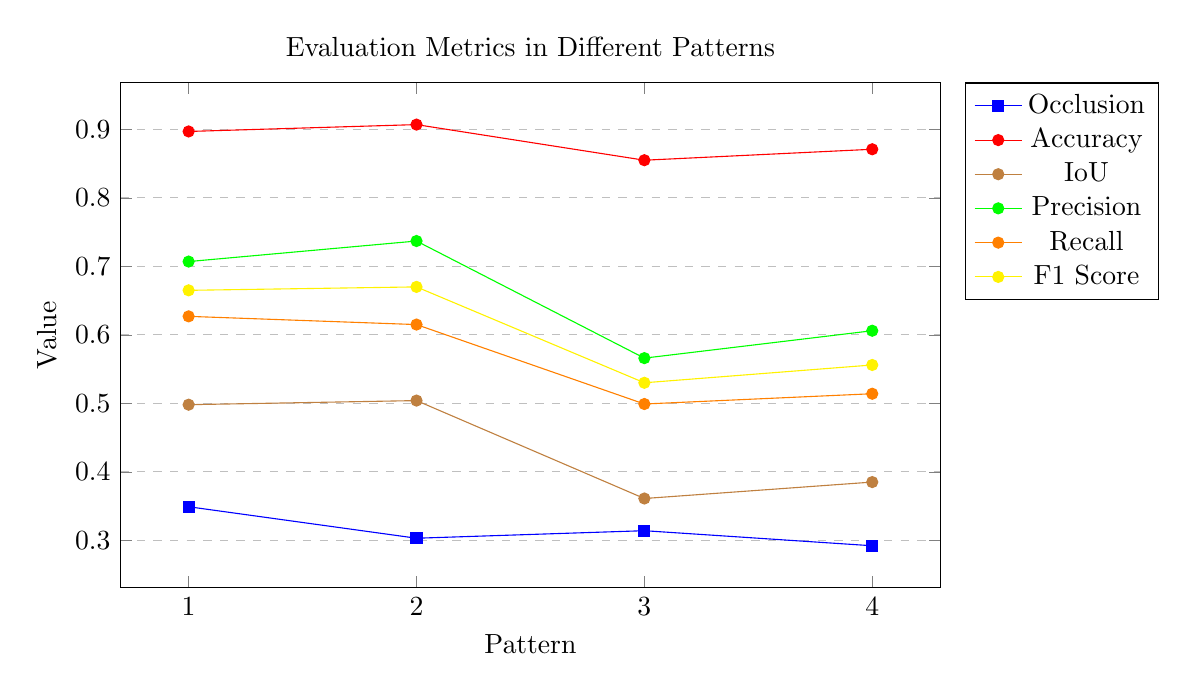
\begin{tikzpicture}
    \begin{axis}[
        title={Evaluation Metrics in Different Patterns},
        xlabel={Pattern},
        ylabel={Value},
        legend pos=outer north east,
        ymajorgrids=true,
        grid style=dashed,
        xtick=data,
        symbolic x coords={1,2,3,4},
        width=12cm,
        height=8cm,
    ]
    
    \addplot[mark=square*,blue] coordinates {
        (1, 0.349)
        (2, 0.303)
        (3, 0.314)
        (4, 0.292)
    };
    \addlegendentry{Occlusion}
    
    \addplot[mark=*,red] coordinates {
        (1, 0.897)
        (2, 0.907)
        (3, 0.855)
        (4, 0.871)
    };
    \addlegendentry{Accuracy}
    
    \addplot[mark=*,brown] coordinates {
        (1, 0.498)
        (2, 0.504)
        (3, 0.361)
        (4, 0.385)
    };
    \addlegendentry{IoU}
    
    \addplot[mark=*,green] coordinates {
        (1, 0.707)
        (2, 0.737)
        (3, 0.566)
        (4, 0.606)
    };
    \addlegendentry{Precision}
    
    \addplot[mark=*,orange] coordinates {
        (1, 0.627)
        (2, 0.615)
        (3, 0.499)
        (4, 0.514)
    };
    \addlegendentry{Recall}
    
    \addplot[mark=*,yellow] coordinates {
        (1, 0.665)
        (2, 0.670)
        (3, 0.530)
        (4, 0.556)
    };
    \addlegendentry{F1 Score}
    
    \end{axis}
    \end{tikzpicture}
    \caption{Evaluation Metrics of Copy Room}
    \label{fig:evaluation metrics of copy room}
\end{figure}

%=====================================================================
\chapter{Conclusion and Discussion} \label{chp:conclusion}
%=====================================================================

\section{Conclusion}

From the results we get from last section, we can find correlation between level of occlusion and segmentation performance.

\section{Discussion}

\subsection{Limitation}

However, there are also many limitations on our work. We cannot assess the occlusion level of a scene very accurately.

\subsection{Future Work}

Some future work can be done to improve our work.

%-------------------------------------------------------------------------------------------------------------------------
\chapter{Acknowledgements} \label{chp:acknowledgements}

Acknowledge any data and code sources you used or for help you received.


%=====================================================================
\chapter*{Document, Writing and Formatting Guidelines}
%=====================================================================

This part of the document uses non-numbered chapter and section headings as they are not part of a regular report structure. In a regular report, \textit{chapters}, \textit{sections} and \textit{subsections} should normally be numbered. Note the use of comment lines and spacings to give more structure to the ASCII text LaTeX document.

In this appendix like part we discuss the structure and formatting rules and guidelines to follow for a written project, research paper, Bachelor or Master thesis report.

%-------------------------------------------------------------------------------------------------------------------------
\section*{Text} \label{sec:text}
%-------------------------------------------------------------------------------------------------------------------------

%-------------------------------------------------------------------------------------------------------------------------
\subsection*{Overall Strategies}

The appearance, clarity and organizational structure of a paper is as important as its technical content, but the technical content must be there beforehand. The presentation alone, however, can make the difference between a mediocre and great publication. Exploit all suitable mechanical rules that can always be applied and optimized independently of the technical part.

The paper has to be convincing even to the adverse reader, i.e. a critical reviewer evaluating your work. Think of being a reviewer yourself, not really knowing your domain and possibly not specifically interested in your work. All information must be crystal clear to a non-expert reader, and all terms and concepts must be properly introduced in a logical order. Put yourself in the position of reading that topic and your work for the very first time, with the goal of having to reproduce it afterwards. The presentation must be flawless and the length of the paper must match the amount of content.

Your report must present your work and solution, best within a convincing story about a difficult problem challenge and an important application domain. The text has to encompass and sell your work. Build up and identify the key challenges in the introduction and problem description. Show clearly how you solved exactly this very important problem in a great and unique novel way.

Group your ideas and concepts hierarchically into sections, subsections and even paragraphs. Strictly introduce general and common ideas, concepts and techniques before expanding further on them. Use the concepts of \emph{repetition} and \emph{parallelism} in your text and structure. The main concept of repetition is to:

\begin{quotation}
Introduce what you are going to tell them -- then tell them in detail -- and finally review what you told them.
\end{quotation}

This approach of repetition is applied on all levels of a report, overall document, sections, subsections and paragraph, always in an appropriate level of abstraction or detail. Example levels:

\begin{description}
\item[Document] The introduction briefly describes the main problem, previews your contribution and summarizes the main results. The main technical sections describe your approach in more detail and the experiments show the achieved results. Finally the conclusion, discussion and future work section(s) summarize your contributions.
\item[Section] In the first paragraph(s) you introduce the topic or aspect that this section covers, followed by the (technical) details, and the last paragraph typically wraps it up, or leads to the next section.
\item[Paragraph] The first sentence of a paragraph leads into the main \emph{message} of this paragraph, and the last sentence concludes it or leads over to the next paragraph.
\end{description}

The concept of parallelism means to apply the same strategy or structuring to different parts. E.g. for each technical problem question or topic covered in one section, first introduce the problem definition and then describe the solution subsequently, possibly in subsections and paragraphs. Or for each type or version of experimental results, or for each data set, describe the data, method parameters, measured variables, report and discuss the results.

It is important to get your text exactly clear to the reader and to avoid the impression that something has been left out or that your contribution is not that significant. But do not over-claim, and more importantly do not under-claim either.

%-------------------------------------------------------------------------------------------------------------------------
\subsection*{Writting and Structure}

Writing is difficult work and usually takes more time than expected. It's beneficial to formalize and write down your progress as early as possible. Generally \emph{you cannot really be sure that you know something until you are able to explain it} well in writing. Hence conveying ideas exactly but in a concise and compact manner is very important and a key to successful writing. Preciseness and compactness are key to be able to describe a large amount of work and results that you have.

Your text must be smooth, forming a clear and logical order of your thoughts and arguments. Use \emph{parallelism} to introduce a set of topics, questions or issues and then elaborate on them subsequently in sections and paragraphs.

Use \emph{repetition}, e.g. introduce the problem, show how to solve it and review the benefits. Do not assume that the reader still remembers what was mentioned only as a passing comment three pages back, use repetition and parallelism.

Do not abruptly jump topics but motivate topic changes. If the topics of text parts change too much, then divide them into subsections or paragraphs. If between paragraphs there are major changes (sequence of different concepts etc.), try to use inline paragraph headings for easy navigation and orientation. One way to integrate such paragraph sequences is to write an introductory paragraph at the beginning of the section and use parallelism.

%--------------------------------------------------------
\paragraph*{Sections and Paragraphs}

Use \textit{sections}, \textit{subsections} and \textit{paragraphs} to structure your ideas and content into meaningful parts, and make a clear and meaningful order of them. Each section, subsection or paragraph must cover a clearly delineated topic or idea.

Every section must first introduce to the reader what to expect and then tell the details, following the principles of repetition and parallelism. An introductory paragraph is also a good approach to fill the space between the section heading and the first sub heading if subsections are used. The last paragraph of a section can summarize the concepts and lead over to the next topic or section.

Each paragraph should have one clear single message, there should only be one consistent topic or idea what the paragraph is about. The first paragraph of a section should clearly lead into the main topic of that section, and the first line of a paragraph should state or at least clearly lead into the main message of that paragraph.

Every single sentence should be fully comprehensible in its context, taking only minimal preliminary knowledge of previous paragraphs into account.

%--------------------------------------------------------
\paragraph*{Wording and Postprocessing}

Use single tenses (i.e. the present or present perfect) as much as possible when describing your design, technical or algorithmic solutions. Generally use present perfect for describing implementations and results which were completed, as this implies something that happened as part of this work in the past but continues to be valid in the present as a result of this paper.

"I" versus "we": For a personal opinion, or your specific personal contribution, you can use the first person. In a personal thesis report one can use "I" as this one's own contribution and text.

For most situations a neutral form should be used, passive voice or third person, but be careful to avoid the interpretation of "passive voice" as "someone else did it, and it is not our contribution", e.g. "This mind-boggling observation was made." vs. "We made this mind-boggling observation.".

Read through the text, spell check, and check the text with a grammar tool as well. Obvious errors are unacceptable.
Try to take the role of a reviewer or evaluator: Reading your paper or report costs that person significant time, so question everything. The reviewer may not be forgiving if something is not clear. Be the devil's advocate!

Do not use abbreviations (don't -> do not).

%-------------------------------------------------------------------------------------------------------------------------
\section*{Formatting and Typesetting} \label{sec:formatting}
%-------------------------------------------------------------------------------------------------------------------------

%-------------------------------------------------------------------------------------------------------------------------
\subsection*{General Rules}

The main text area should have a margin of about 2cm on both sides, and the main text should have a top and bottom margin of about 3cm each.

Section and subsection headings have nested numbering and are typeset in sans-serif bold font type, e.g. Helvetica or Arial.  Sizes range from 18pt for main sections down to at least one point larger than the main body text size. Some vertical space before and after section headings is placed (automatically according to the LaTeX document class of this template).

The main body text is typeset in 11pt Times font (serif font family). Text body is one-column, justified and single-spaced. First line of a paragraph is generally indented with about 0.8cm, however, first paragraph after any section heading may also be non-indented.

\begin{itemize}
\item Avoid extensive and manual spacing
\item Use font modifications carefully
%\item Use the \verb!\emph{}! command fo emphasizing/italicizing not \verb!\textit()!
\item Use proper math and symbol styles
%\item Use (our math.tex) style file for consistency
\end{itemize}

%-------------------------------------------------------------------------------------------------------------------------
\subsection*{Folder Structure}

Use main folder for the main latex .tex and .bib files, the main paper body and bibliography database. Optional: use a folder, e.g. ./sections, to separately manage individual section's latex files.

Use ./images and ./figures subdirectories for the raster images and vector graphics used in the figures and diagrams of the paper.
Only use .jpg and .pdf formats respectively for best results. Put source files, e.g. from Illustrator or OmniGraffle, also directly into the ./figures folder along with the PDF versions.

%-------------------------------------------------------------------------------------------------------------------------
\subsection*{Latex Coding}

Follow a clear prologue structure in the LaTeX source file. After the given template components add your \verb!\usepackage{}! block, and \verb! \def\mathbi#1{\textbf{\em #1}}
 
% commands
\newcommand{\Adjoint}{\mbox{\rm Adj}}
\newcommand{\Area}{\mbox{\rm Area}}
\newcommand{\ACos}{{\mbox{\rm Cos}^{-1}}}
\newcommand{\ASin}{{\mbox{\rm Sin}^{-1}}}
\newcommand{\ATan}{{\mbox{\rm atan2}}}
\newcommand{\Code}[1]{{\tt #1}}
\newcommand{\Complex}{\mbox{\bf C}}
\newcommand{\Cross}{{\mbox{\rm Cross}}}
\newcommand{\Mydddot}[1]{\mbox{\shortstack{$.$\hspace*{-1pt}$.$\hspace*{-1pt}$.$\\$#1$}}}
\newcommand{\Degree}{\mbox{\rm degree}}
\newcommand{\Diag}{\mbox{\rm Diag}}
\newcommand{\Dim}{\mbox{\rm dim}}
\newcommand{\Dist}{\mbox{\rm Distance}}
\newcommand{\IntTwo}{\int\!\!\int}
\newcommand{\IntThree}{\int\!\!\int\! \!\int}
\newcommand{\Kernel}{\mbox{\rm kernel}}
\newcommand{\Kross}{\mbox{\rm Kross}}
\newcommand{\Grad}{\nabla}
\newcommand{\Perp}{\mbox{\rm Perp}}
\newcommand{\Point}[1]{{\cal #1}}
\newcommand{\Rank}{\mbox{\rm rank}}
\newcommand{\Range}{\mbox{\rm range}}
\newcommand{\Real}{{\mbox{\rm I}\hspace*{-2pt}\mbox{\rm R}}}
\newcommand{\RealSbt}{{\mbox{\rm\scriptsize I}\hspace*{-2pt}\mbox{\rm\scriptsize R}}}
\newcommand{\Res}{\mbox{\rm resultant}}
\newcommand{\Sbt}[1]{{\mbox{\rm\scriptsize #1}}}
\newcommand{\MySign}{\mbox{\rm Sign}}
\newcommand{\SignSBT}{\mbox{\rm\scriptsize Sign}}
\newcommand{\Skew}{\mbox{\rm Skew}}
\newcommand{\Span}{\mbox{\rm Span}}
\newcommand{\SqrDist}{\mbox{\rm Distance$^2$}}
\newcommand{\Trace}{\mbox{\rm Trace}}
\newcommand{\TRN}{{\mbox{\rm\scriptsize T}}}
\newcommand{\Vector}[1]{\mbox{\bf #1}}
\newcommand{\VectorM}[1]{\mbox{\boldmath $#1$}}
\newcommand{\Volume}{\mbox{\rm Volume}}

\newcommand{\IVec}{\mbox{\boldmath $\imath$}}
\newcommand{\JVec}{\mbox{\boldmath $\jmath$}}
\newcommand{\KVec}{\mbox{\boldmath $k$}}
\newcommand{\LVec}{\mbox{\boldmath $\ell$}}
\newcommand{\RMat}{{\cal R}}
\newcommand{\QMat}{{\cal Q}}
\newcommand{\QCMat}{\overline{\cal Q}}

\newcommand{\Lerp}{\mbox{\rm lerp}}
\newcommand{\Slerp}{\mbox{\rm slerp}}
\newcommand{\Quad}{\mbox{\rm quad}}
\newcommand{\Squad}{\mbox{\rm squad}}

\newcommand{\ODer}[2]{\frac{d #1}{d #2}}
\newcommand{\ODerT}[2]{\frac{d^2 #1}{d {#2}^2}}
\newcommand{\ODerM}[3]{\frac{d #1}{d #2 \, d #3}}
\newcommand{\PDer}[2]{\frac{\partial #1}{\partial #2}}
\newcommand{\PDerT}[2]{\frac{\partial^2 #1}{\partial {#2}^2}}
\newcommand{\PDerM}[3]{\frac{\partial^2 #1}{\partial #2 \, \partial #3}}

% mass density symbol
\newcommand{\Den}{\delta}

% environments
\newenvironment{BArray}[1]{\left\{ \begin{array}{#1}}{\end{array} \right\}}
\newenvironment{Combin}{\left( \begin{array}{c}}{\end{array} \right)}
\newenvironment{Matrix}[1]{\left[ \begin{array}{#1}}{\end{array} \right]}


\let\mbf=\mathbf
\let\mvec=\mathbf
\let\mcal=\mathcal
\let\mfunc=\mathrm

%\def\R{\mbox{\ensuremath{\mathrm{I\!R}}}}
\newcommand{\R}{\ensuremath{\mathbb{R}}}
\newcommand{\N}{\ensuremath{\mathbb{N}}}
\newcommand{\Z}{\ensuremath{\mathbb{Z}}}
\newcommand{\C}{\ensuremath{\mathbb{C}}}

\newcommand{\of}[1]{\left( #1 \right)}
\newcommand{\abs}[1]{\left| #1 \right|}
\newcommand{\norm}[1]{\left\Vert {#1} \right\Vert}
\newcommand{\gradient}[1]{\nabla{\!}_{#1}{\,}}
\newcommand{\twovec}[2]{\left( #1 \atop #2 \right)}
\newcommand{\threevec}[3]{\left(\begin{array}{c}#1\\#2\\#3\end{array}\right)}
\newcommand{\fourvec}[4]{\left(\begin{array}{c}#1\\#2\\#3\\#4\end{array}\right)}

\newcommand{\refsec}[1]{Section~\ref{sec:#1}}
\newcommand{\reffig}[1]{Fig.~\ref{fig:#1}}
\newcommand{\reftab}[1]{Tab.~\ref{tab:#1}}
\newcommand{\refeq}[1]{Eq.~(\ref{eq:#1})}

%\newcommand{\R}{\hspace*{0.1ex}{\sf I} \hspace{-0.3ex}{\sf R}}

%6.5
\newcommand{\eps}{\mbox{$\epsilon$}}
\newcommand{\dmin}{\mbox{$d_{\min}$}}
\newcommand{\dmax}{\mbox{$d_{\max}$}}
\newcommand{\dminmax}{\mbox{$[\dmin,\dmax]$}}

%4.2:
\def\M{\mathcal{M}}
\def\n{\mathbi{n}}
\def\p{\mathbi{p}}
\def\q{\mathbi{q}}
\def\x{\mathbi{x}}
\def\tp{^{\mathsf{T}}}

\let\vec=\mathbi%
\let\mat=\mathbf%
\let\set= \mathcal%
! to include our standard math formula definitions. Complete the preamble by any further specific definitions or commands, e.g. \verb!\TODO! and \verb!\FIXME! macros. After the prologue, complete the title and author parts.

If separate .tex files are used for the main report text body, then include them in the main body latex file, and in each of these files indicate the root latex file at the very top:
\begin{verbatim}
%\!TEX root = ../<main_file_name>.tex!
\end{verbatim}

\noindent
Further LaTeX coding guidelines and recommendations:

\begin{itemize}
\item Use the \verb!\emph{}! command fo emphasizing/italicizing not \verb!\textit()!
\item Use (our math.tex) style file for math formula consistency
\item Use \verb!\mathrm{function()}!  for function names
\item Use consistent section, equation and figure labelling
\verb!\label{sec:introduction}! as well as \textit{eq:rendering, fig:system}
\item Do not liberally introduce manual horizontal or vertical spacings
\item In particular do not use comment codes \% to control spacing or indentation before or after elements, e.g. arounc equations, figures or tables
\end{itemize}

%-------------------------------------------------------------------------------------------------------------------------
\subsection*{Mathematical Formulas and Equations}

Mathematical expressions should follow a consistent set of rules, symbols and formatting as indicated in our \textit{math.tex} style file. LaTeXiT can be used for consistent symbols and formulas in figures. Apply the same scalar, vector and matrix styles as well as use the same variables consistently throughout your text, see also the predefined styles and specific variables in \textit{math.tex}. A few guidelines that are useful are given below, use them as much as possible (but adjust as necessary to make formulas clear):

\begin{itemize}
\item use (lower-case) italic letters for normal (scalar) variables such as $x$ or $t$
\item prefer $i$ and $j$ as index variables and $m$ and $n$ to denote number of elements or iterations
\item use for example other letters such as $a$, $b$ and $c$ for constants
\item use lower-case bold italic to denote vectors such as $\vec{u}$ or $\vec{v}$
\item use upper-case bold letters such as $\mat{M}$ or $\mat{N}$ for sets and matrices
\item use upper- or lower-case italic letters such as $f()$ or $G()$ to denote functions
\item use regular plain font and decimal point to denote explicit constants such as $2$ or $100.12$
\end{itemize}

Use as much formalism, variables and equations, as is useful to clearly understand your description, but not for trivial facts. Use inline equation format also for variables like $x$ and numbers like $12$ used in the main text body segments.

Mathematical equations that are important or are referenced should be laid out as a  regular equation with consecutive numbering to the right as below:

%% example equation  %%
\begin{equation}
E = m \cdot c^2
\label{eq:einstein}
\end{equation}

Such regular free standing equations do not need a punctuation and follow a paragraph that ends with a dot or double-colon, and the following paragraph starts regularly indented.

Equations may also be treated 'inline' with the main flow of the text, thus being part of one regular sentence. Such 'inline' equations as
%
\begin{equation*}
a^2 + b^2 =  c^2,
\end{equation*}
%
typically end with a comma and the text continues below unindented lower-case to finish the sentence. To adjust spacing, the equation can be connected to the paragraph text flow by separating it only using \% comments. If an equation ends the sentence of a paragraph it ends with a dot.


%-------------------------------------------------------------------------------------------------------------------------
\subsection*{Floats, Figures, Screenshots and Graphs}

Figures, screenshots, tables, graphs and other floats should support the overall idea of the paper or some description in the text specifically, and are numbered sequentially. Every figure must support a key idea or concept, and it must be meaningful with self-explanatory captions.

\begin{quotation}
Make sure every figure or float is placed correctly and is used as well as referenced in the text.
\end{quotation}

\paragraph{Placement}
Each float is centered and \emph{placed in the text directly after} the first paragraph referencing it, never directly after a heading. If formatting constraints are difficult, figure placement may be forced, e.g. to be placed at the top of the next possible new page.
In double-column document formats, put large floats spreading both columns at the top of the next following page.

\paragraph{Figures}
Use a consistent style and appearance for each figure, using clean lines and diagrams. Make careful use of not too bright or disturbing colors, and watch out for grayscale usage when printed.

Use sans-serif fonts in figures and diagrams unless for math symbols and variables. Enforce consistent upper-lower case usage throughout all figures and terms used in the text, and match variables and math formulas or symbols in figures to the ones in in the text. Also match the size of text in figures to the size of the main paper body text.

For figures and diagrams that include any vector graphics elements (e.g. arrows, lines, boxes, points etc.), use the PDF vector graphics format with white or transparent background, and do not use raster image formats. If raster images are included in vector graphics figures, also use the PDF format for the combined figure.

\paragraph{Screenshots}
Each screenshot must demonstrate a clear visual effect, or major point of your work, or an example or problem of a standard (prior) approach. Some, very few, images may be mostly visual teasers. Each screenshot must include all details such as (data) statistics, used parameters and experimental settings in the caption or in the accompanying text where the figure is referenced from. Use raster image formats only for image-only figures, and then use the JPG file format not PNGs.

\paragraph{Graphs}
Graphs and plots must clearly demonstrate some numerical test results or data statistics. Strictly avoid clutter within one graph, and clearly relate parameters and results of experiments. Just listing basic values can be done in simple tables.
Use expressive and clearly labelled axis in all graph plots. Graphs should basically be understandable on their own along with their caption also without reading the main text. Graphs and plots are usually based on vector graphics, thus use the PDF vector graphics format with white or transparent background as for figures and diagrams.

%-------------------------------------------------------------------------------------------------------------------------
\subsection*{Cross-References}

Cross-references to numbered items such as sections and figures are capitalized as in the following examples. In Section~\ref{chp:introduction} we provide a brief summary of text formatting instruction and Figure~\ref{fig:logo} shows our group logo. A figure can contain multiple subfigures which can be referenced individually as illustrated in Figure~\ref{fig:uzh}.

%% example figures %%
\begin{figure}[htp]
 \centering
 \includegraphics[width=0.5\textwidth]{figures/vmml_logo}
 \caption{Example of single figure with caption text.}
 \label{fig:logo}
\end{figure}

\begin{figure}[htp]
 \centering
\subfigure[vmml logo]{\includegraphics[width=0.3\textwidth]{figures/vmml_logo} \label{fig:vmml}} \hfill
\subfigure[uzh logo]{\includegraphics[width=0.3\textwidth]{figures/uzh_logo} \label{fig:uzh}}
 \caption{Example subfigure with captions referencing (a) the VMML and (b) the UZH logos.}
\end{figure}

Use the same full or shortened form for all references, e.g. Sec.~\ref{chp:introduction}, Fig.~\ref{fig:vmml}, Eq.~\ref{eq:einstein}.

%-------------------------------------------------------------------------------------------------------------------------
\subsection*{Pseudo Code}

Example for a pseudo code given below

%% example pseudo code %%
\lstinputlisting[language=c++,label=example]{pseudocode/example_pcode.txt}
\vspace{10mm}

%-------------------------------------------------------------------------------------------------------------------------
\subsection*{Commands}

You can use the command \verb!\FIXME{}! in order to mark sections in the text, which need to be edited and fixed. E.g. \FIXME{check reference XY}.


%-------------------------------------------------------------------------------------------------------------------------
\section*{Bibliography}
%-------------------------------------------------------------------------------------------------------------------------

The bibliography with list of references is placed on a new page at the end of the document, titled ``References'' or ``Bibliography'' and typeset similar to the main section headings but without numbering. Bibliography entries should follow standard IEEE or ACM proceedings or transaction journal formatting styles, and be referenced by last name abbreviation and year such as e.g. \cite{Pajarola:07} and \cite{GSSP:10}, or by number as for [1].

%-------------------------------------------------------------------------------------------------------------------------
\subsection*{Formatting References}


Bibliography entries should be clean, accurate, compact and consistent across all entries. Thus for the entries in the BibTeX bibliography .bib file follow the following basic rules:

\begin{itemize}
\item Have complete entries, including full author names (first and last), full conference paper (inproceedings type with name, year, pages) and journal (article type with journal name, volume, number/issue, month) data
\item Use capitalized title and special terms, e.g. "Point Set Processing for Data Analysis on the {GPU}".
\item Use consistent venue description (name the same conference/journal in the same way).
\item Use compact \emph{inproceedings} booktitle for conferences without year, i.e. "Proceedings IEEE Visualization" instead of "8th Int. Conference on Visualization (VIS'08), IEEE 2008".
\item Do not use separate organization field if clear from the conference or journal, and usually no publisher, month and address for conferences.
\item Keep entries concise, avoid unnecessary or duplicate information such as e.g. address or location for conferences or even journals, redundant numpages fields, or duplicated association/organization data etc.
\item Use these fields sparsely if at all necessary: howpublished, publisher (don't for conferences, only for books or so), series (don't for conferences, only for LNCS or similar)
\item Typically do not use venue, address or location for conferences or even journals
\item Keep keywords simple and meaningful (e.g. main first keyword graphics, visualization, geometry, theory, databases, mathematics etc. followed by a few more specific ones)
\end{itemize}

\noindent
Example bad BibTeX entry:

\begin{verbatim}
@ inproceedings{as78439729asf,
  Title = {Tile-based LOD for the Parallel Age},
  Author = {Niski, Krzysztof and Cohen, J.~D.},
  Booktitle = {Proceedings IEEE Visualization Conference (IEEE Vis'10)},
  Volume = {13},
  Pages = {1352},
  Organization = {IEEE},
  Series = {IEEE TVCG journal},
  Publisher = {Computer Society Press},
}
\end{verbatim}

\noindent
Above BibTeX entry will result in a not very nice, incomplete and inconsistent reference:

\smallskip
\noindent
[NC] Krzysztof Niski and J. D. Cohen. Tile-based lod for the parallel age. In \emph{Proceedings IEEE Visualization Conference (IEEE Vis'10)}, volume 13 of \emph{IEEE TVCG journal}, page 1352. IEEE, Computer Society Press.

\bigskip
\noindent
The corresponding clean and consistent BibTeX entry would be:

\begin{verbatim}
@article{NC:07,
  Title = {Tile-based {LOD} for the Parallel Age},
  Author = {Niski, Krzysztof and Cohen, Jonathan~D.},
  Journal = {IEEE Transactions on Visualization and Computer Graphics},
  Month = {November/December},
  Volume = {13},
  Number = {6},
  Pages = {1352--1359},
  Year = {2007}
}
\end{verbatim}

\noindent
This will result in a nice and consistent reference:

\smallskip
\noindent
[NC07]  Krzysztof Niski and Jonathan D. Cohen. Tile-based LOD for the parallel age. \emph{IEEE Transactions on Visualization and Computer Graphics}, 13(6):1352-1359, November/December 2007.

\vspace{5mm}
More bad examples include the following
\begin{quotation}
\cite{HWH:10bad,Suss:10bad,HXS:09bad,CH:09bad,Strugar:10bad,Fout:07bad,WGS:07bad,CMF:05bad,AGLMR:02bad,Koltun:00bad,CYHPK:97bad}, 
\end{quotation}

and the good ones are these here
\begin{quotation}
\cite{HWH:10,SWF:10,HXS:09,CH:09,Strugar:10,FM:07,WGS:07,CMF:05,AGLMR:02,KCC:00,CYHPK:97}.
\end{quotation}


%=====================================================================
\chapter*{Pages}
%=====================================================================


%-------------------------------------------------------------------------------------------------------------------------
\section*{Cover and Abstract}
%-------------------------------------------------------------------------------------------------------------------------

Title of thesis, author, affiliation, date and any other administrative information should be placed on a separate cover page (see first page).

Main title of work should be typeset in large sans-serif bold font type. Title is to be followed by author and affiliation. At the bottom, separated group affiliation is set.

Abstract follows on separate page after cover page and before the table-of-content page(s).


%-------------------------------------------------------------------------------------------------------------------------
\section*{TOC}
%-------------------------------------------------------------------------------------------------------------------------

The table-of-content (TOC) contains all Section and (Sub-)Sub Section headings and their corresponding pages and is listed on separate pages before the first section. It has its own heading typeset as a section heading without numbering.

%%=====================================================================
%\chapter{Conclusion} \label{chp:conclusion}
%%=====================================================================
%
%Summarize your main findings in one or maximum two pages. Try to keep yourself short and clear. Give a short discussion about your results where you focus on what your findings mean. E.g., show how your results and interpretations agree with the original question and with other published work  or if there are any possible practical applications for your work. At the end, give hints on further improvements or development directions / areas. 

\bibliographystyle{alpha}
\bibliography{references,bad_refs,corrected_refs}
\end{document}
